
{\chapter{Exploring the single-cell RNAseq analysis landscape in timeseries patient derived xenografts}

}
 \label{ch:Chapter5}
 \section{Motivation}

%\printinunitsof{in}\prntlen{\textwidth}
%\printinunitsof{in}\prntlen{\textheight}
% The text width is 6.5in -- important for plotting
% The text height is 9in

To further enhance our understanding of how fitness under drug treatment occurs, we sought to identify genomic and non-genomic basis for transcriptome differences. 
In TNBC, copy number changes have a major influence on the expression landscape \cite{wang2016integrative}.
Although many studies have analyzed CNV and differential gene expression of distinct oncogenes and tumor suppressor genes in various cancers \cite{kuzyk2015mycn, budczies2016pan, kwak2015fibroblast}, yet there has been no precise study about the relationship between CNV and differential gene expression across multiple tumor samples. It is unclear to what extent the expression level is affected by CNV at single cell level.
In Chapter 4, we established a system for identifying copy number defined clones and here we intend to exploit that to obtain scRNA-seq from the clones by mapping 10x with clonealign to CNA genotypes \cite{campbell2019clonealign}.

As \ac{DLP+} allows identification of regions of the genome that differ between the clones and the regions that are similar \cite{laks2019clonal}, therefore, we would be able to define which regions of the transcriptome might be influenced by CNA driven expression and those that might be independent of change in copy number state.

Because of the difficulty to analyse longitudinal patient samples for single cell gene expression and the lack of multiple longitudinal pre-clinical breast cancer models, these questions remain unexplored and our understanding of how they relate to triple negative breast cancer heterogeneity is limited.

Here we aimed to systematically investigate the specific relationship between copy number change and differential gene expression across timeseries TNBC PDX for which we have clonal copy number proportions already analysed in chapter 4. 

%In spite of advanced technologies and treatment, triple negative breast cancer still faces the problems of tumor recurrence and drug resistance.
%For any given difference between the types of drug resistance, for example the expression of a particular gene, it is assumed that differences arise deterministically or probabilistically in the presence of transcription factors regulating the genes in the tumors. Cancer cells in distinct cell states often exhibit important differences in functional properties depending on which genes are turned on and off resulting in sensitive or resistant phenotypes.

%The most challenging analysis is to differentiate whether the change in gene expression leading to change in cellular state is stochastic \cite{raj2008nature} or deterministic to produce the same output under similar environment.
%Previously it was shown that unique cells within a population can exhibit fluctuations in gene expression that could predict distinct phenotypes \cite{shaffer2019memory}.

%We set to explore 3 timeseries breast cancer patient derived xenografts (PDX) that were serially challenged for around 4-5 cycles with one or two drugs until and beyond they started showing resistant behaviour. The aim is to measure the magnitude of fluctuations in gene expression from sensitive to resistant phenotype.
%This study may help us better understand the correlation between CNV and differential gene expression and provide new insights into the mechanism of development and progression of cancers with potential biomarkers in triple negative breast cancer.

 \section{Synopsis}

The overall goal of this chapter is to determine the impact of change in copy number on the phenotype. By using single cell RNA sequencing in conjunction with clonealign  \cite{campbell2019clonealign}, a proportion of the genome  was defined that was affected by copy number dependent transcription.
 
 This chapter is divided into 3 sections of data evaluation, copy number dependent transcriptome proportions and changes over time. Highlights in synopsis are followed by detialed results: 
  
  \subsection{ScRNA-seq data processing and evaluations for downstream analyses} 
\begin{itemize}
  
   \item Generated scRNA-seq data for 145,858 single cells across 3 triple negative breast cancer timeseries PDX 
(TNBC-SA609, TNBC-SA1035, TNBC-SA535) that were serially challenged for 4-5 cycles of (cisplatin) platinum and SA535 additionally with CX-5461 to create resistance.
   \item \texttt{edgeR} and SCTransform were strongly correlated for normalization of all 3 timeseries data with TNBC-SA609 having the highest correlation coefficient between them.
 \item Normalization with SCTransform partially removed batch effects with a small range of mean gene expression differences.
 \item Relative abundance of copy numbers assigned scRNA-seq clonal subpopulations were strongly correlated.
 \item Single cell copy number clonal structure observed in UMAP was able to summarize transcriptomes with residual batch effects.

\end{itemize}
\subsection{Contrasts of resistant and sensitive clone specific gene 
expression reveals the rates of in cis and in trans components} 
\begin{itemize}
   
   \item Copy number change \textit{in cis} expression accounts for $\sim${6.3\%-38.52\%} of clonal differences in resistant vs sensitive transcriptomes. The overall number of \textit{in trans} genes were higher as compared to \textit{in cis}, which was consistent with previously reported results.
 
 
 %\item For all DE comparisons, DE in-cis genes average was 38.52\% (sd=11.43) for SA609, SA535 cisplatin, SA535 CX5461,  however, the proportion of DE in-cis genes for SA1035: average was 6.3\% (sd= 0.92).
 
 
 
 \item  In 4 published cancer fitness and cisplatin resistance datasets, DE genes showed  highest match \textit{in cis} of TNBC-SA535, in both treatment regimes with 28\% maximum. Whereas, TNBC-1035 had the lowest match with 2.4\%.

 \item Overall, out of 100\% of \textit{in cis} regulated genes, the highest average of positive linear up or down regulation with copy number was found in TNBC-SA1035 with average of 88.3\% (sd=3.9) and lowest in TNBC-SA609 with average of 74.1\% (sd=13.2). 
 %TNBC-SA535-cisplatin, SA535-CX-5461 showed 83.7\% (sd=6.5) and  85.7\% (sd=3), respectively.
 
 \item Cisplatin resistance associated genes were observed in the extremes of the distribution, for example \textbf{COX6C, PI3, UQCRB, ATP5MPL, CSDE1, CXCL3, S100P, S100A7, HERC5, IFITM3, NDUF and  CRABP1}.
 
  \item Commonly upregulated pathways in TNBCs-SA609, SA535-cisplatin and SA535-CX-5461 included \textbf{TNF, EMT, TGF beta, HYPOXIA, APOPTOSIS, E2F, MITOTIC SPINDLE and ESTROGEN  RESPONSE}, whereas, \textbf{OXPHOS} was downregulated. 
 
 \item \textbf{OXPHOS and INTERFERON pathways} were only upregulated  in TNBC-SA1035.

\end{itemize}

\subsection{Change in gene expression over time}

\begin{itemize}
 \item Most of the chemoresistance associated pathways were activated in the later passages with repeated exposure to drugs.
 
 \item Drug holiday samples showed a shift towards untreated expression, for example, drug holiday samples of \textit{in cis} regulated \textbf{UQCRB (OXPHOS pathway)},  and drug holidays samples of \textit{in trans} regulated, \textbf{MYC (MYC targets V2)}.
 \item Line trajectories of individual genes over time showed that expression change could be monotonically increasing or decreasing under drug selection, for example, \textit{in cis} regulated \textbf{VDAC3  (OXPHOS pathways)} and in trans regulated, \textbf{BTG1 (TNFA via NFKB pathway)}.
 %\item In TNBC-SA535, common precursor clone R, in comparison with untreated sensitive clone, showed additional upregulation of HEDGEHOG and ANDROGEN RESPONSE pathways in TNBC-SA535.

 \item Line trajectories of individual genes over time showed that expression change could be monotonically increasing or decreasing under drug selection, for example, in cis regulated VDAC3, from OXPHOS pathways and in trans regulated, BTG1 from TNFA via NFKB pathway.

\end{itemize}

\begin{figure}
\centering
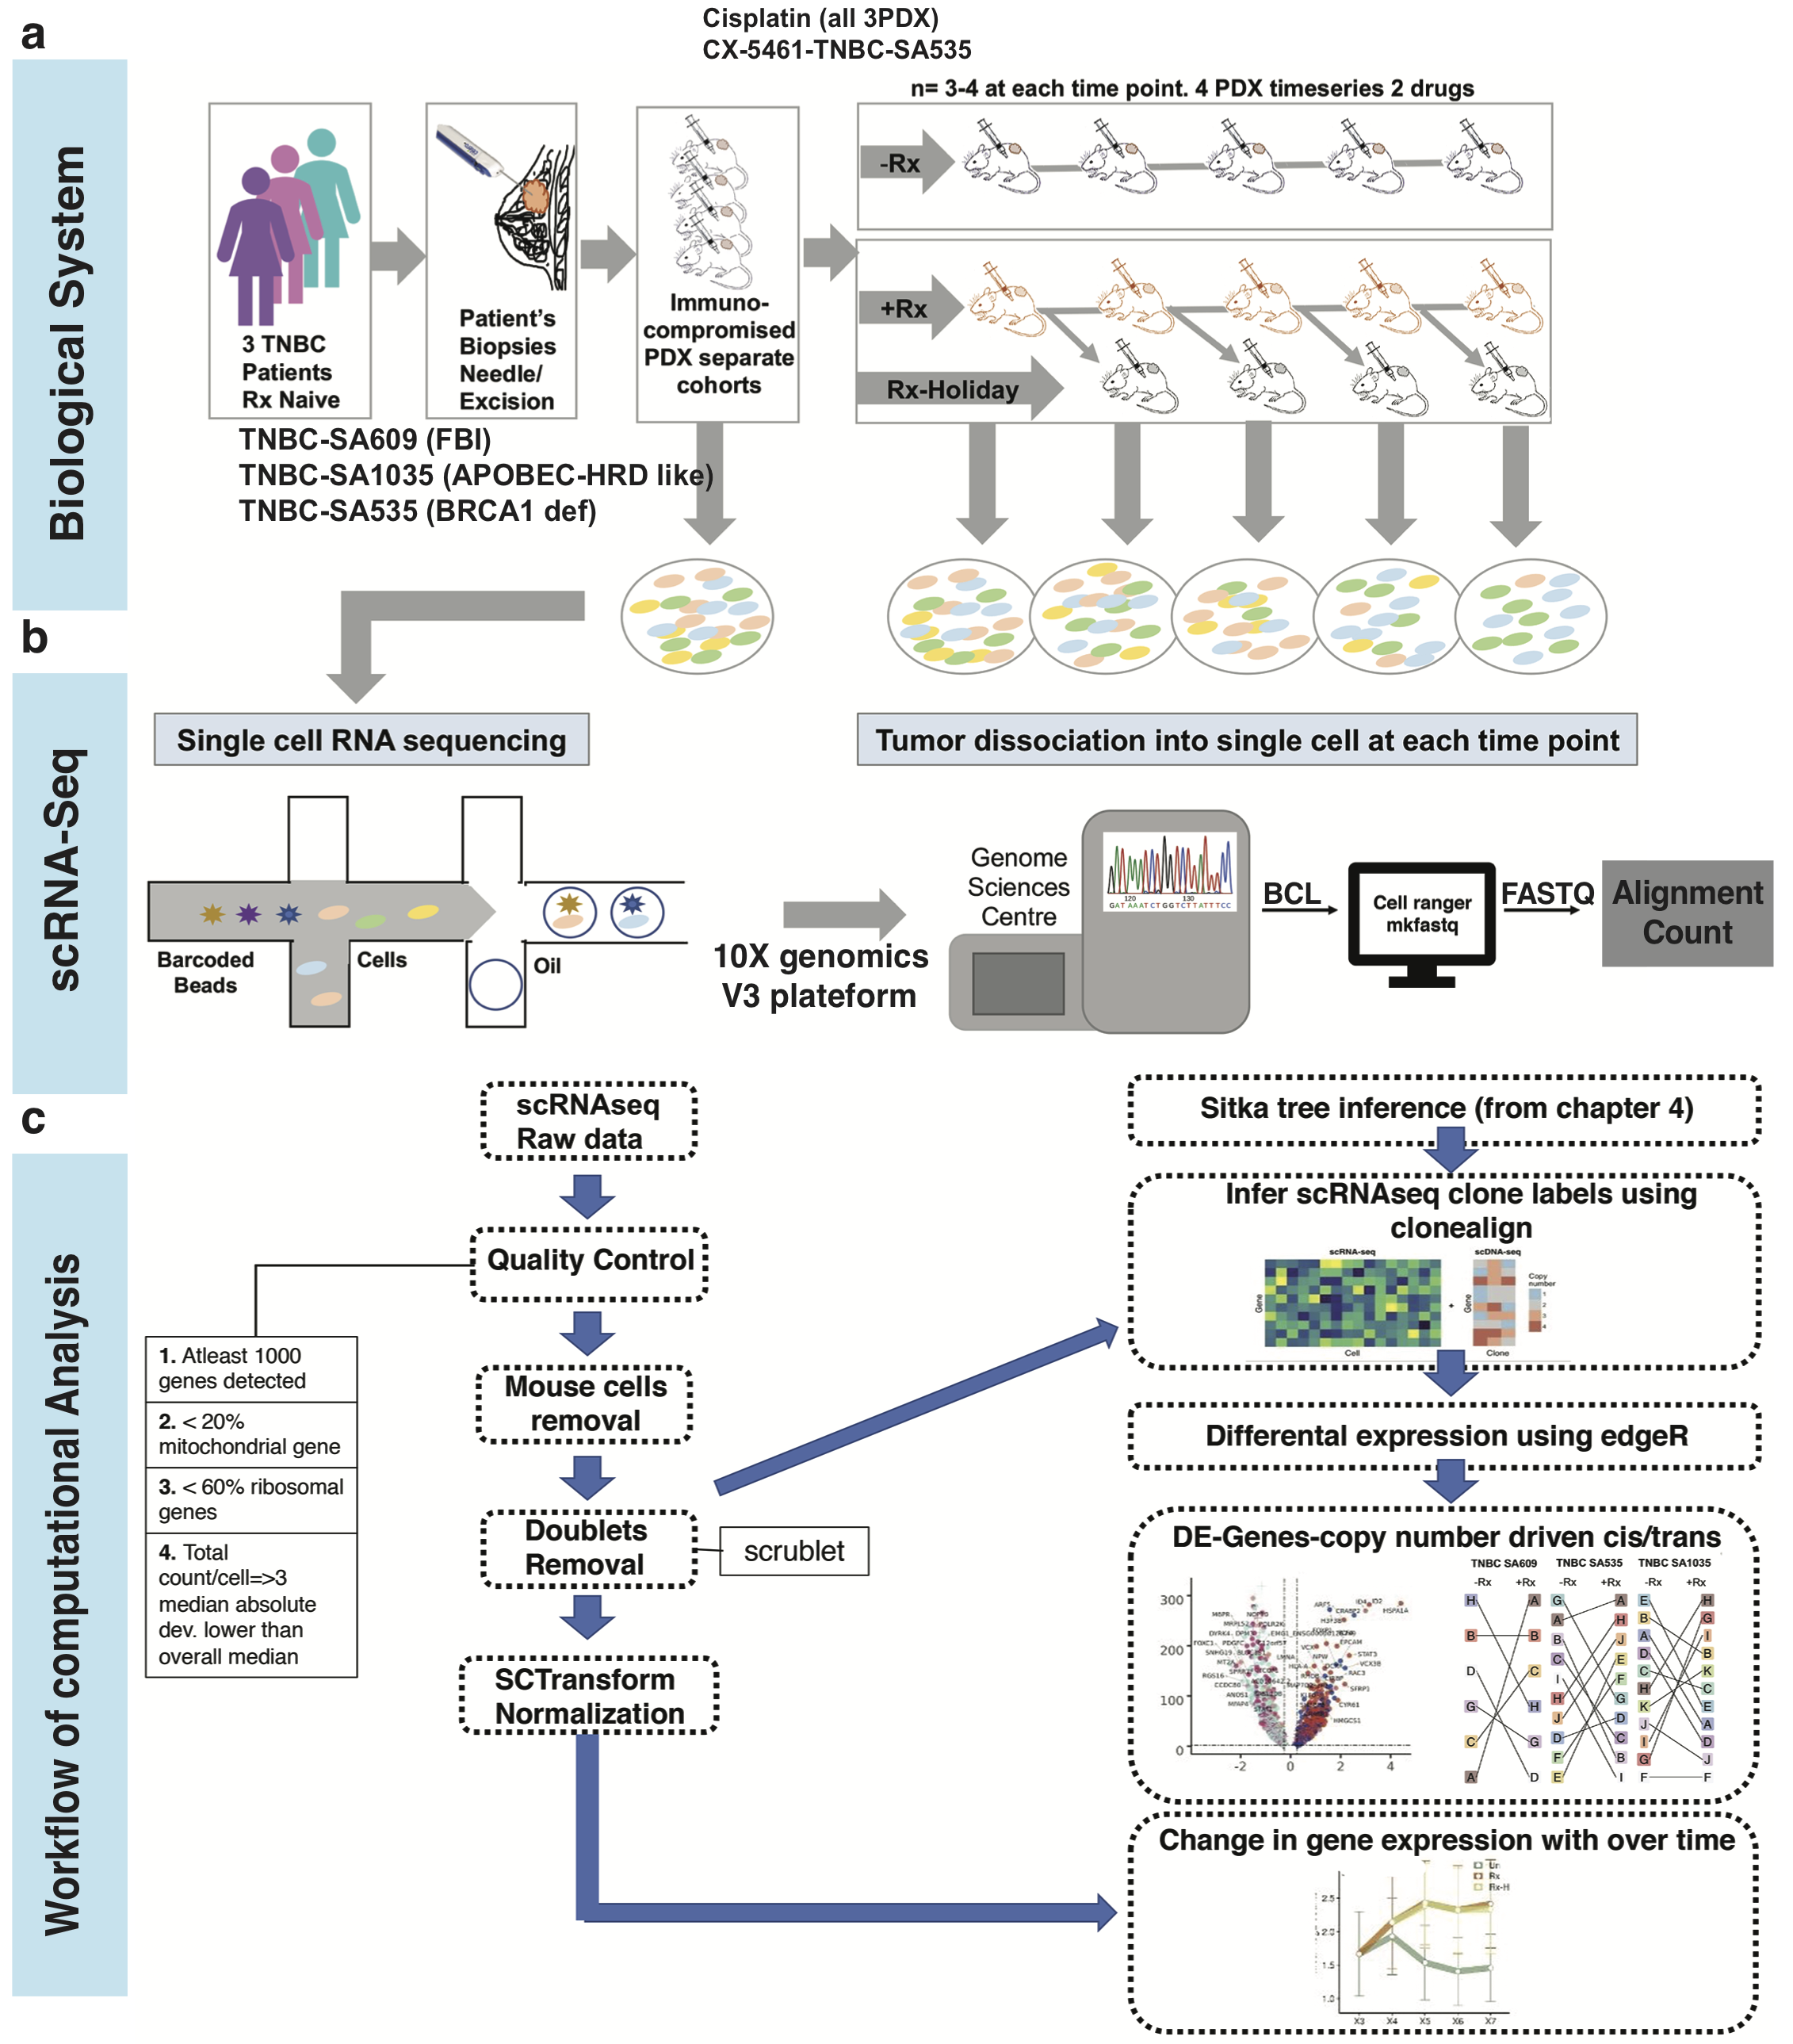
\includegraphics[width=\textwidth]{Figures/chap5/RNAworkflow.png}
	
\caption[Schematics of experimental design and analysis workflow]
	{\small
	\textbf{Schematics of data generation and analysis workflow.}
	   \textbf{(a)} Overview of the experimental design same series as of chapter 4.
	    \textbf{(b)} Single cells RNA library prep. and sequencing.
	    \textbf{(c)} Computational workflow analysis used in this chapter.
	}
	\label{fig:chap5RNAworkflow}
\end{figure}
%----------------------------------------------------------------


\section{Results}
 

%\subsection{Longitudinal single-cell RNA sequencing of patient-derived xenografts}
\subsection{Data collection and processing sets the ground for biological analyses} 
  
\subsubsection{Sample collection and workflow of data generation and analysis from triple negative breast cancer timeseries PDX}
To understand resistance at the single cell RNA level, we selected 4  patient-derived xenograft timeseries that were developed by transplanting patient's tumor biopsies in immunodeficient mice as described in chapter 3 (\textbf{\autoref{fig:chap5RNAworkflow} a}). 
Briefly, 3 triple negative breast cancer xenografts (TNBC-SA609, TNBC-SA1035,TNBC-SA535) were serially challenged for 4-5 cycles of (cisplatin) platinum compound to create resistance.
Similar to aforementioned experiments for chapter 4, we collected exactly same tumors to digest and generate single cell RNA libraries using Chromium 10X genomics (chemistry V3) Single Cell 3' Reagent Chemistry kit standard protocol. Libraries were then sequenced on an Illumina Nextseq500/550. The sequenced raw data was passed through the following bioinformatic analysis pipeline: 
%for downstream exploration of single cell gene expression in all timeseries (\textbf{\autoref{fig:chap5RNAworkflow} c}) 
Binary base call (BCL) files are the raw data files generated by the Illumina sequencers. Cellranger mkfastq demultiplexes BCL files into FASTQ files. Cell ranger is a set of analysis pipelines that process Chromium single-cell RNA-seq output to align reads to human genome GRCh38 and generate featured-barcode matrices. Cellranger count takes FASTQ files from cell ranger mkfastq and performs alignment, filtering, barcode counting, and UMI counting (\textbf{\autoref{fig:chap5RNAworkflow} b}). 

Next, low quality cells were removed and only cells that passed the threshold of quality control were kept. 
 \texttt{scater} package was applied for quality control filters. Cells were considered to be good quality if (i) at least 1000 genes detected, (ii) less than 20\% of counts (UMIs) mapping to genes from the mitochondrial genome (``mitochondrial genes''), (iii) fewer than 60\% of counts (UMIs) mapping to ribosomal genes, and (iv) the total counts (UMIs) per cell was at most 3 median absolute deviations lower than the overall median. Cells not matching all criteria were filtered using the \ac{QC} Metrics and Outlier functions in the \texttt{scater} package \cite{mccarthy2017scater}.

Next, clonal assignments from \texttt{sitka} tree inference from chapter 4 was used to run clonealign \cite{campbell2019clonealign} for \ac{scRNAseq} clone labels. Moreover, \texttt{SCTransform} \cite{hafemeister2019normalization} and \texttt{edgeR} \cite{robinson2010edger}, were applied for normalization and differential gene expression analysis, respectively (\textbf{\autoref{fig:chap5RNAworkflow} c}). 


%---------------------------------------------------------------
\begin{table}[htbp]
 \centering
  \caption{Number of cells sequenced for transcriptome analysis}
{
\begin{tabular}{|l|r|r|}
\hline
Sample labels     & No. of cells sequenced for scRNA & Filtered \\
\hline
Untreated         & 52,256                           & 21,510    \\
Cisplatin-Rx      & 40,754                           & 19,095    \\
Cisplatin-holiday & 31,269                           & 15,158    \\
CX-5461-Rx        & 8,558                            & 4,047     \\
CX-5461-holiday   & 13,021                           & 3,373  \\  
\hline
Total cells          & 145,858                          & 63,183\\
\hline
\end{tabular}%
\label{tab:nofcellsRNA}
}
\end{table}
%----------------------------------------------------------------

 %-------------------------------------------------------------
 
\subsubsection{Summarization of number of cells and overall read counts of the data}
Tumors from each time point of TNBC-SA609, TNBC-SA1035 and TNBC-SA535 (cisplatin, CX-5461) were collected and enzymatically digested with collagenase/hyaluronidase at 37\textdegree C, for single cell RNA sequencing as DLP+ (\textbf{\autoref{fig:RNAsampletree}}). In chapter 3, it was described that tumor dissociation with collagenase enzyme at warmer temperature produces stress response that is minimized
by dissociation at cold temperature. For the experiments of this chapter, we preferred to use collagenase enzyme because the tumor dissociation, for chapter 4 DLP+ libraries, were also done using the same enzyme. Also, the chemotherapies are also known to produce stress responses and we didn't want to mask the expected biological responses by known technical effects. 
%need to fill in the proper number and table from Mirela
From the scRNA-seq libraries, the cells obtained per line ranged from 1111 to 222222 after filtering for high quality cells, representing X to Y cells per time point sample, median Z \textbf{\autoref{tab:nofcellsRNA}}. 


\textbf{\autoref{fig:Diagnosticplotsreadcounts}} shows medians of features by counts (number of genes with non-zero counts value) range from 3826 to 4878 (interquartile range of (3109 to 6320).and total counts per cell medians range from 14043.6 to 27805.5 over all samples (interquartile range of 4342.2 to 63899) in all 4 TNBC-PDX timeseries. 

%\begin{itemize}
   % \item Series SA609: total counts - median over all samples: 14043.6 interquartile range: [4508-17752.2]   number of genes with non-zero counts - median over all samples: 4283.9 interquartile range: [3109-6053]
%\item Series SA1035: total counts - median over all samples: 21935.2 interquartile range: [4342.2-48549.8]   number of genes with non-zero counts - median over all samples: 3826 interquartile range: [2013-5366] 
%\item Series SA535:Cisplatin: total counts - median over all samples: 27805.5 interquartile range: [10453.8-63899]   number of genes with non-zero counts - median over all samples: 4878.7 interquartile range: [3236-6320]
%\item Series SA535:CX5461: total counts - median over all samples: 26869 interquartile range: [17787.2-35371]   number of genes with non-zero counts - median over all samples: 4286.2 interquartile range: [3603.5-6057]

%\end{itemize}

The large variablity between samples is in part due to batch processing effects in sequencing depth per cell and number of cells obtained pointing to the need for batch correction/normalization.


%Only 2 libraries in TNBC-SA1035 (X5-UT-CHIP0071 and X5-UU-CHIP0076) had a low quality cells than other libraries (~2500 total features by counts) but acceptable and good enough to use. Other exceptions were TNBC-SA535-CX-5461 treated at time points X7 and X9 with low quality, that was excluded from the downstream analysis. 

%----------------------------------------------------------------

\begin{figure}
\centering
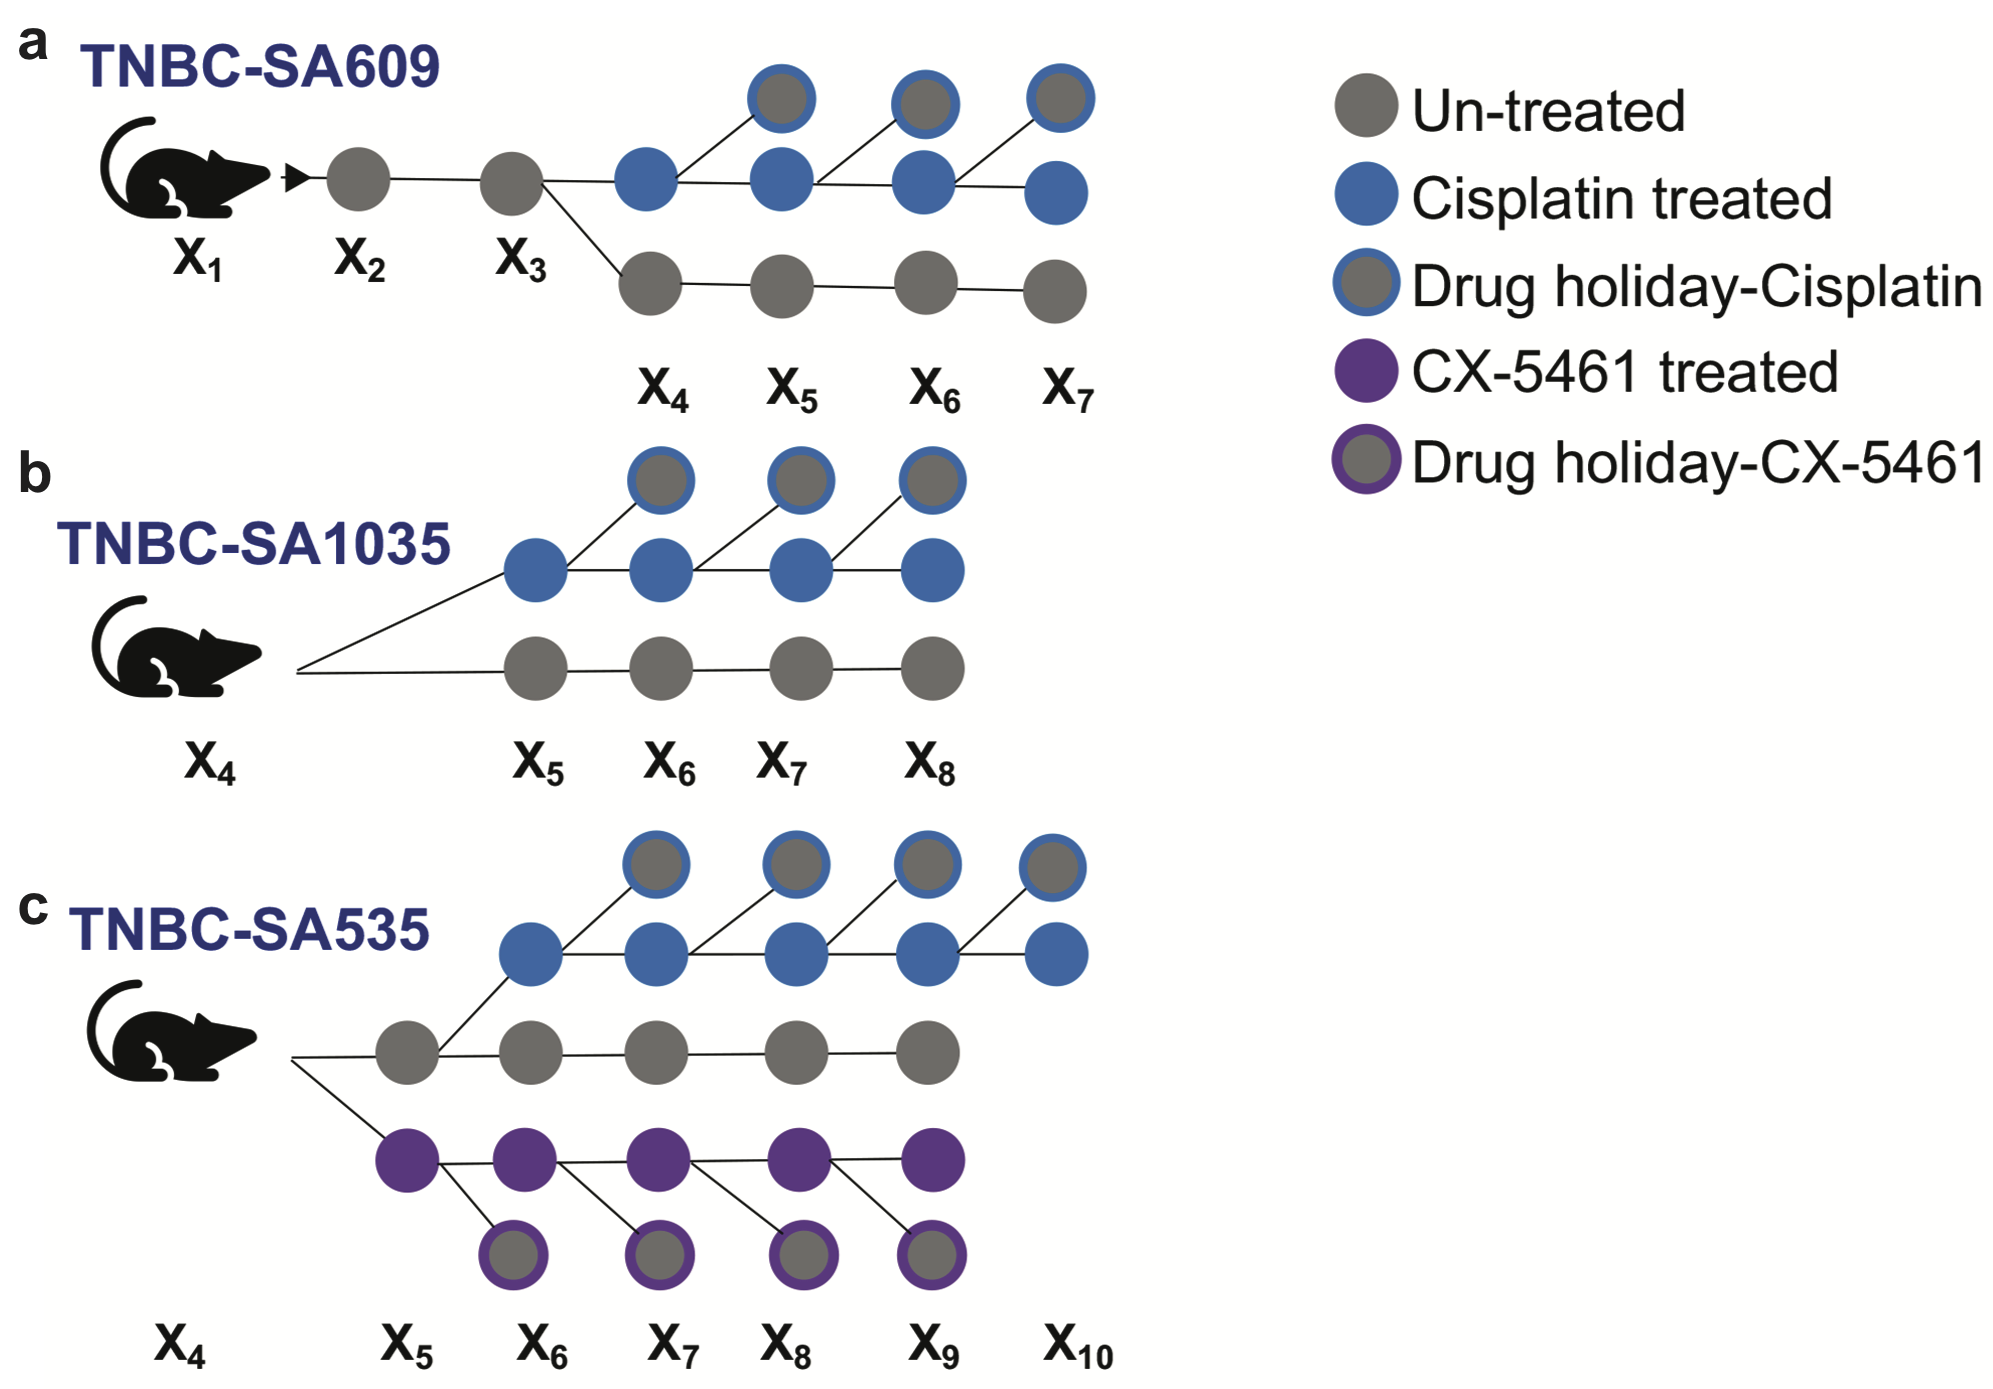
\includegraphics[width=\textwidth]{Figures/chap5/SchematicsforRNAsampling.png}
	
\caption[SchematicsforRNAsampling]
	{\small
	\textbf{Time series sampling and treatment conditions used for scRNA-seq analysis.}
	Each circle indicates patient derived xenograft tumor. All blue circles denote cisplatin treated tumors while purple circles denote CX-5461 treated tumors. Grey with blue outline are ciplatin drug holiday samples while grey with purple outline present CX-5461 drug holiday tumors. X with subscript numbers indicates the respective passage number of that time series. 
	   \textbf{(a)} TNBC-SA609.
	    \textbf{(b)} TNBC-SA1035.
	    \textbf{(c)} TNBC-SA535.
	}
	\label{fig:RNAsampletree}
\end{figure}

%---------------------------------------------------------------

\begin{figure}
\centering
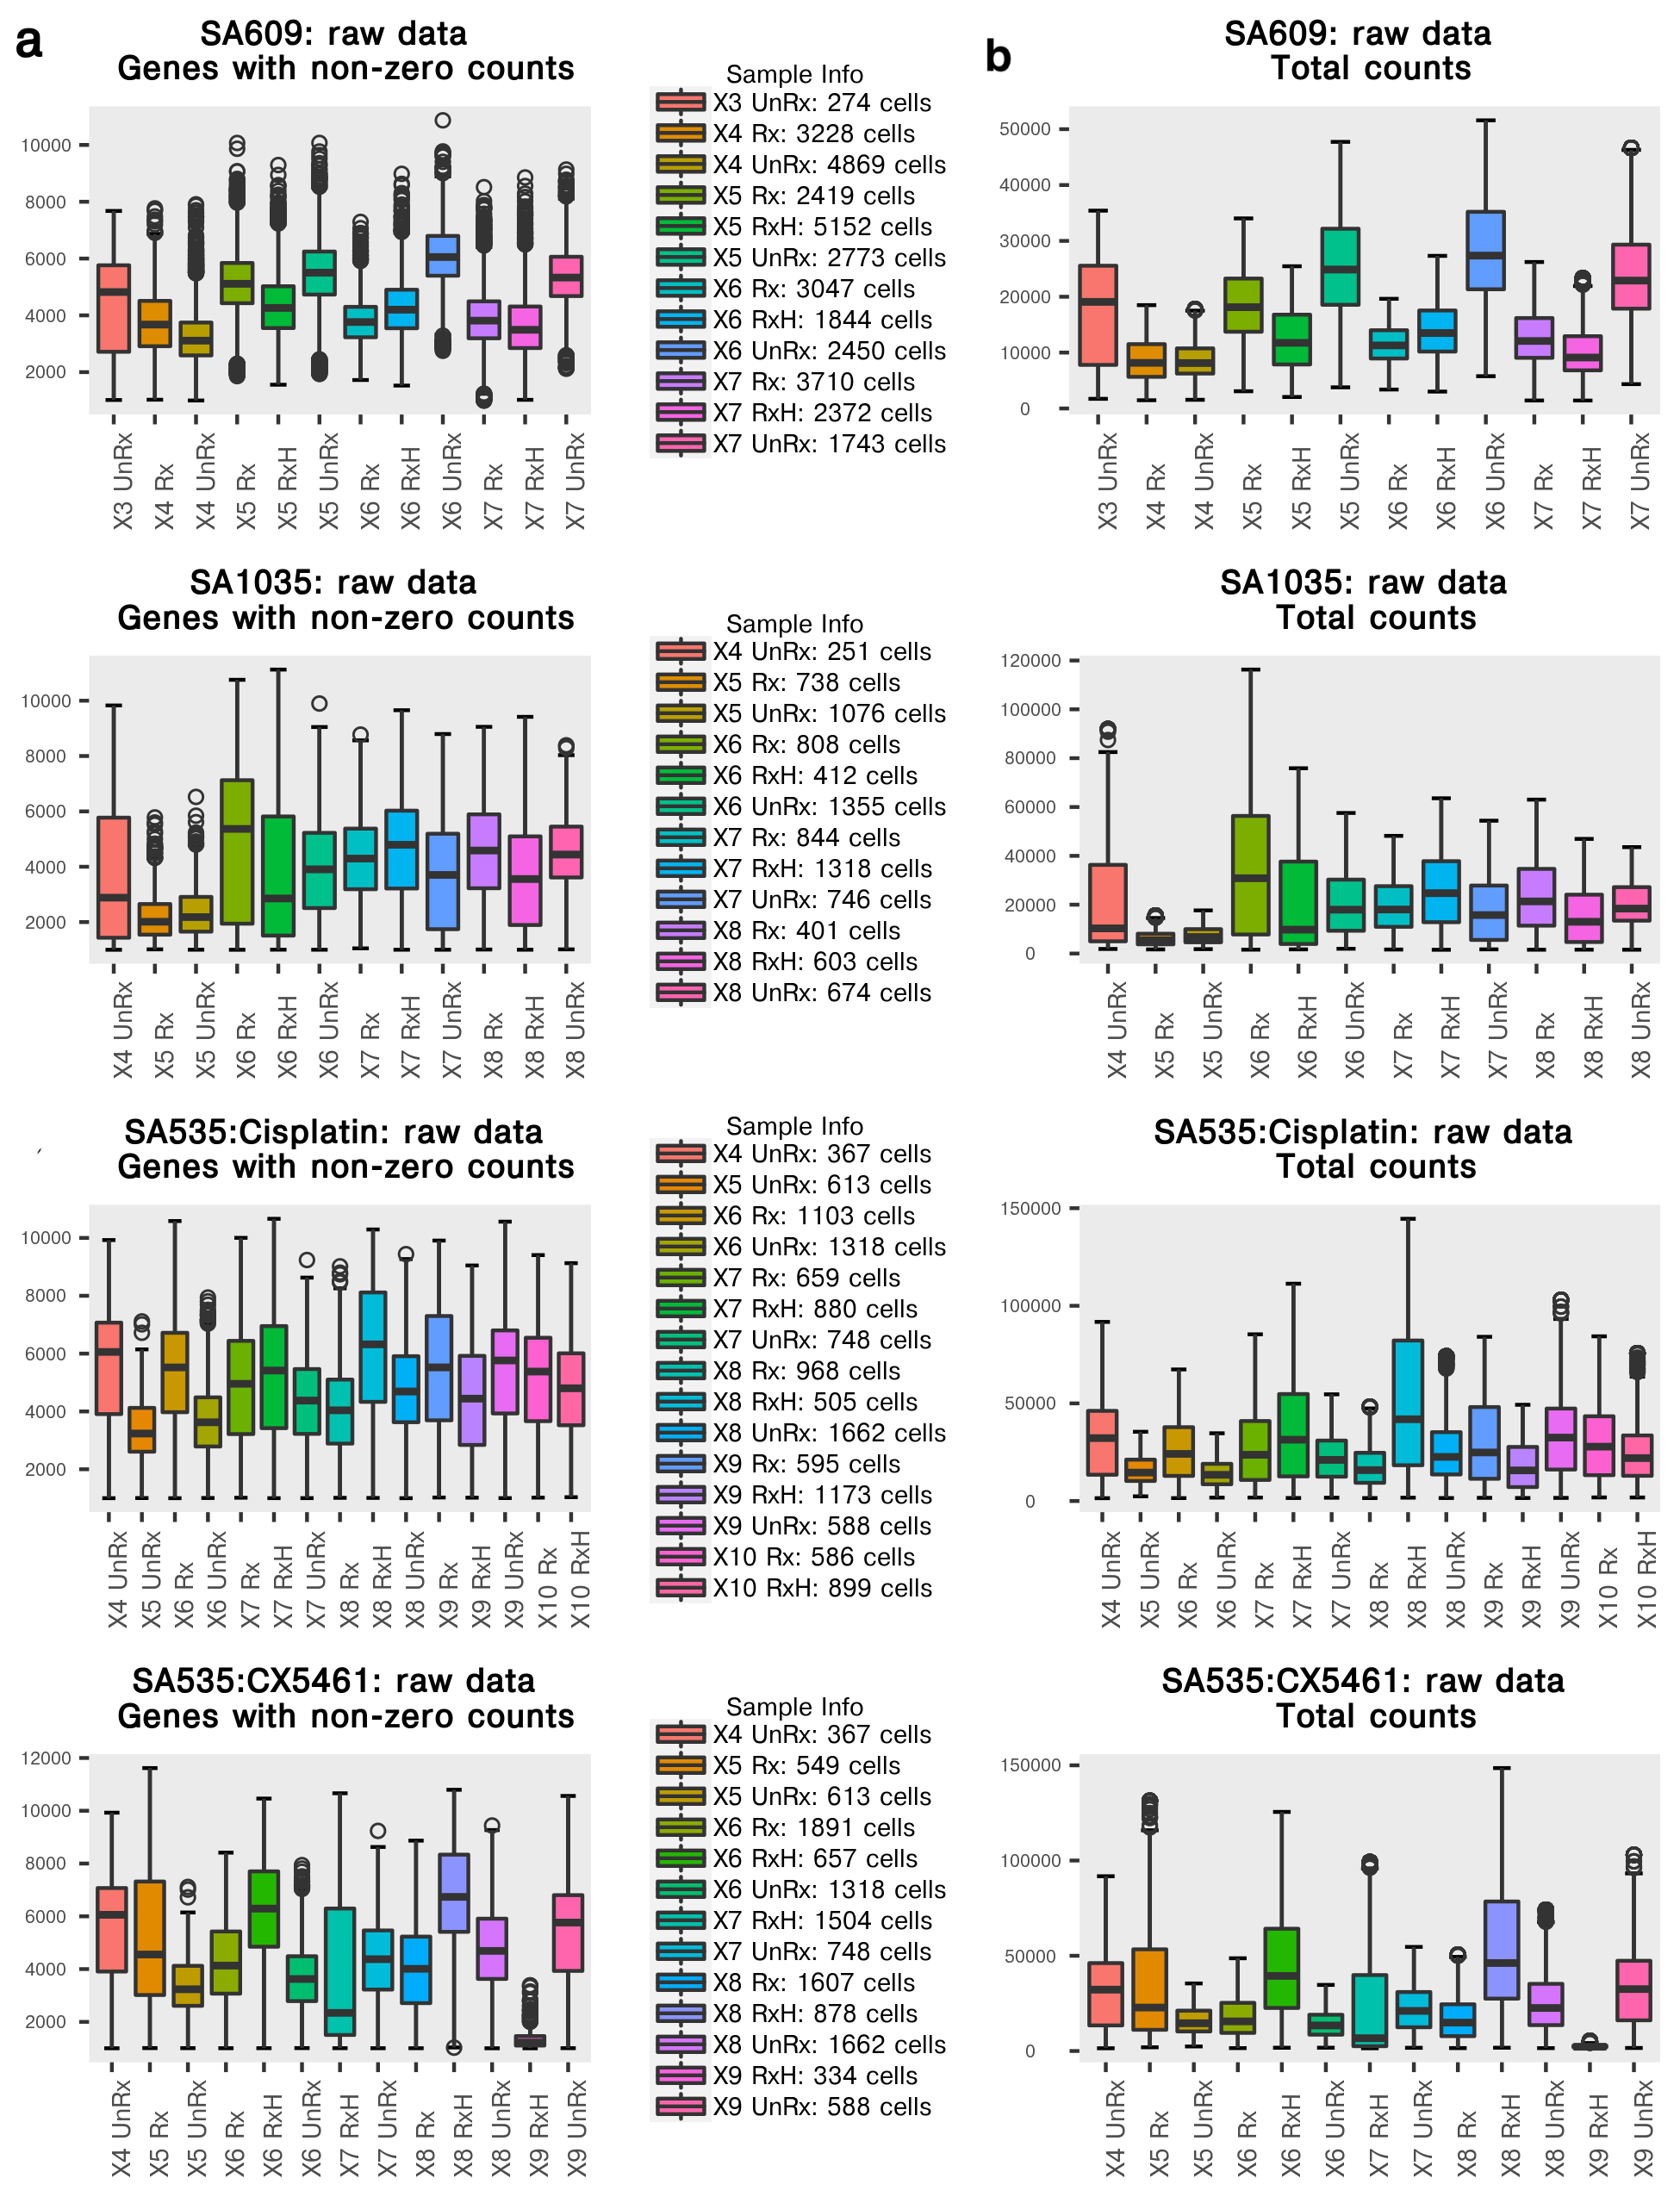
\includegraphics[width=\textwidth]{Figures/chap5/Diagnosticplotsreadcounts.png}
	
\caption[Summary of overall read counts and features of the raw data presented.]
	{\small
	\textbf{Summary of overall read count of the data presented.}
	   All Horizontal axis denotes different batches of experiments
	   \textbf{(a)} Number of ``genes with non-zero counts'' for all batches of experiments. 
	    \textbf{(b)} Cell level metric ``total cell counts'' for all batches of experiments.
	   
	}
	\label{fig:Diagnosticplotsreadcounts}
\end{figure}

%-----------------------------------------------------------

\begin{figure}
\centering
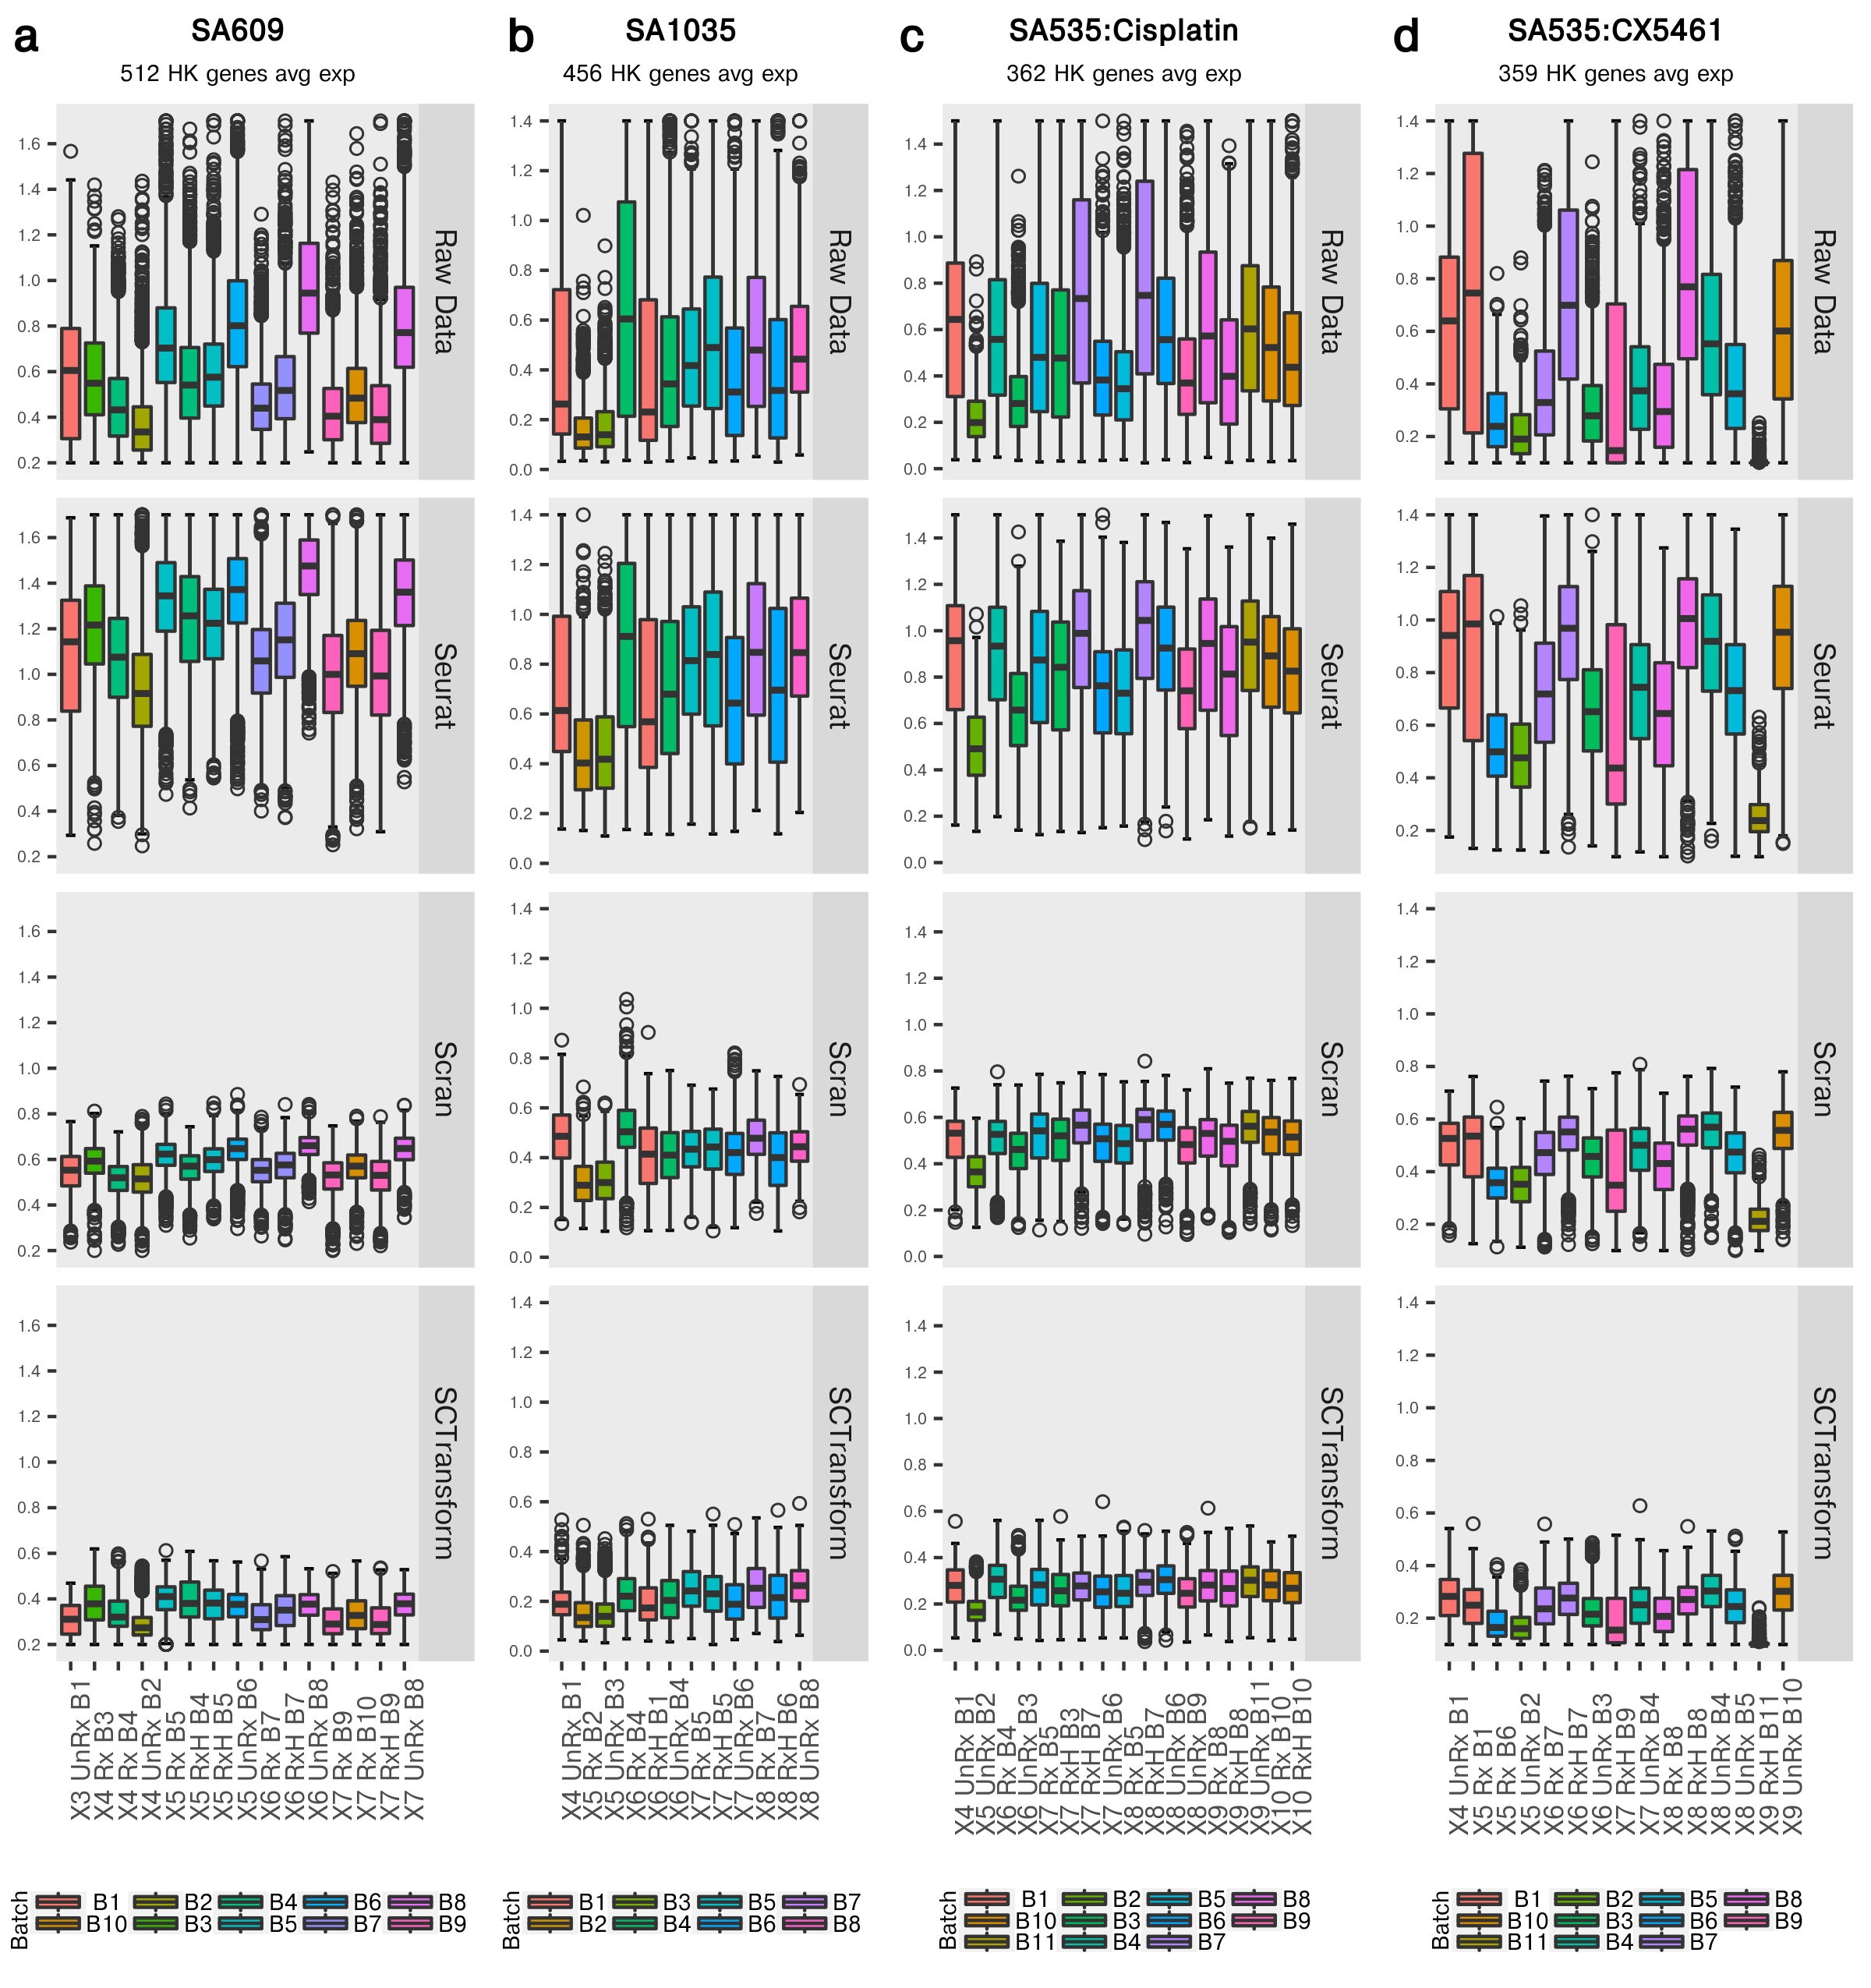
\includegraphics[width=\textwidth]{Figures/chap5/Comparisonofbatcheffects.png}
	
\caption[Summary of overall read count of the data presented.]
	{\small
	\textbf{Evaluation of batch effects in TNBC PDX timeseries data.}
	  House keeping genes were selected from \cite{lin2019evaluating} and mean expression calculated in all timeseries of TNBC PDX. Horizontal axis shows sample IDs from each of that time series and vertical axis shows mean gene expression.
	   \textbf{(a)} Raw data with no normalization showing mean expression of house keeping genes in all 4 treated and untreated TNBC PDX timeseries. 
	    \textbf{(b)} Two times applying scran on data (Twice scran) normalization  in all 4 treated untreated TNBC PDX timeseries.
	    \textbf{(c)} Suerat (normalization) on  all 4 treated and untreated TNBC PDX timeseries.
	    \textbf{(d)} SCTransform (normalization) on  all 4 treated and  untreated TNBC PDX timeseries
	}
	\label{fig:Comparisonofbatcheffects}
\end{figure}
%-----------------------------------------------------------------

\begin{figure}
\centering
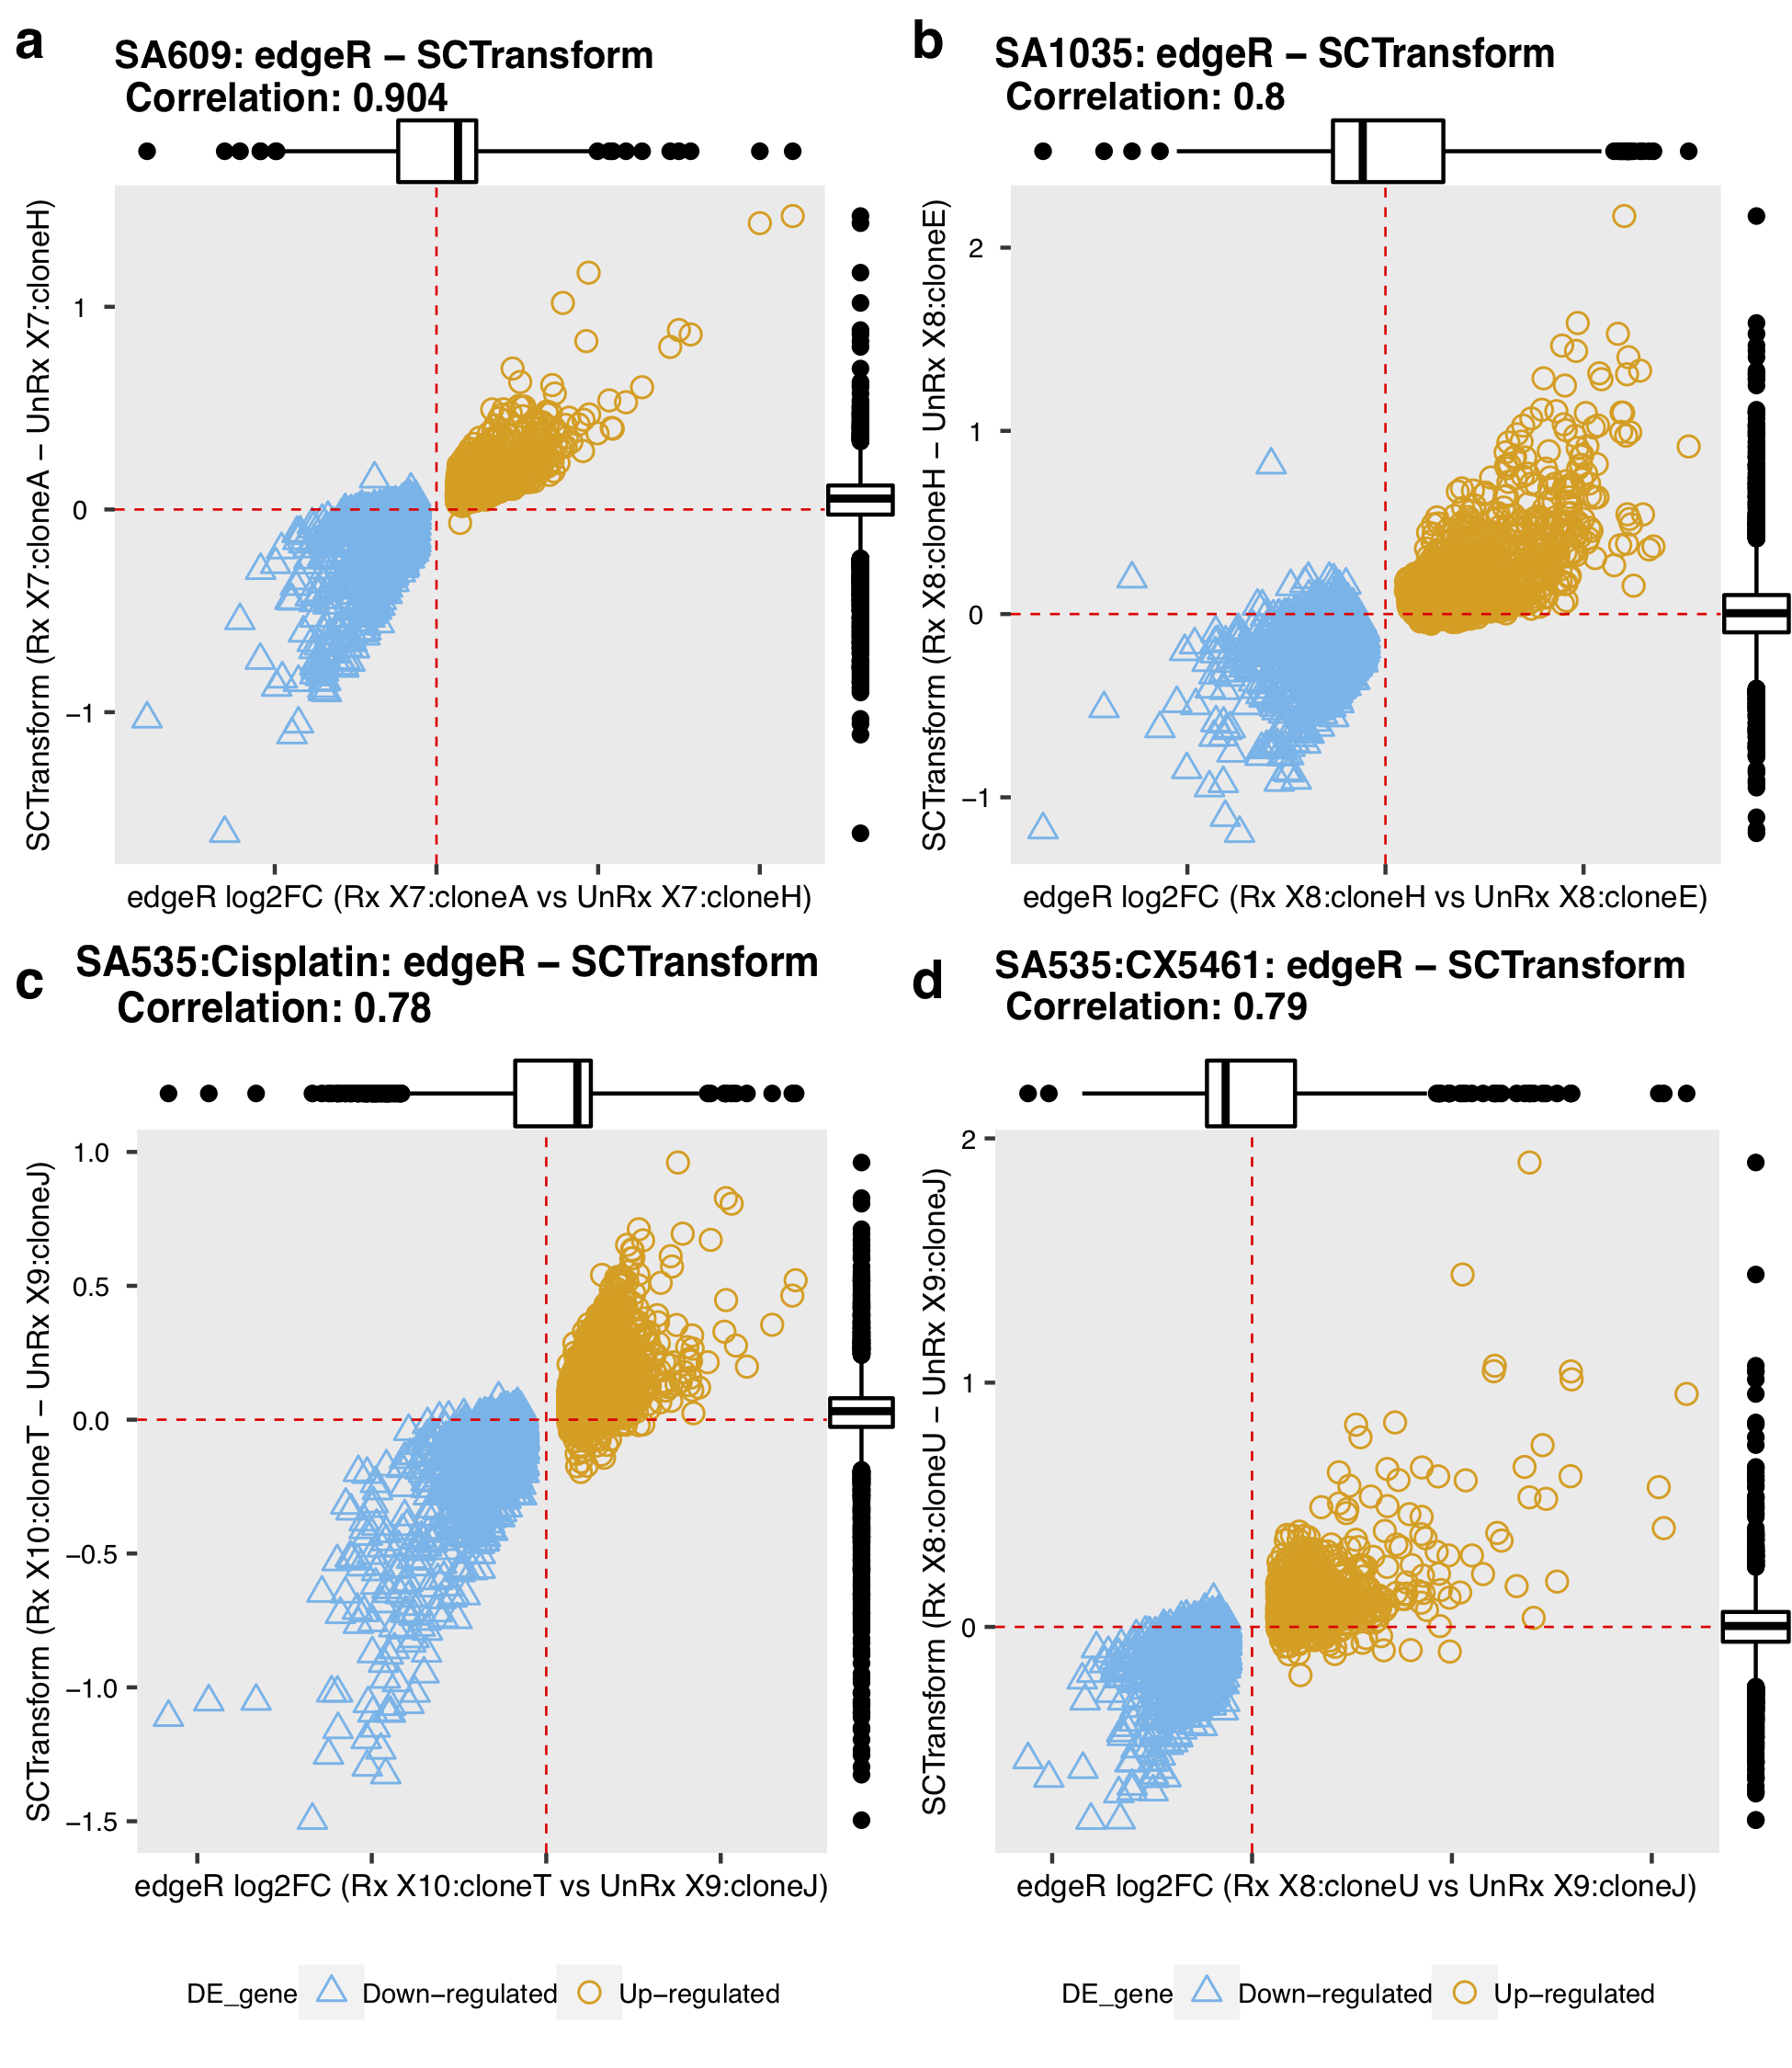
\includegraphics[width=\textwidth]{Figures/chap5/edgeRSCTransformcorrelation.png}
	
\caption[Evaluation of \texttt{edgeR} in all PDX timeseries data.]
	{\small
	\textbf{Comparison of edgeR with SCTransform normalization for downstream data analysis.}
All vertical axis presents SCTransform normalized logcounts genes expression in resistant clone versus logcounts genes expression in sensitive clone. All horizontal axis presents log base 2 fold change of gene expression of \texttt{edgeR}.	
	}
	\label{fig:edgeRsctransformcorrelation}
\end{figure}

%-------------------------------------------------------------

 %------------------------------------------------------------------


\begin{figure}
\centering
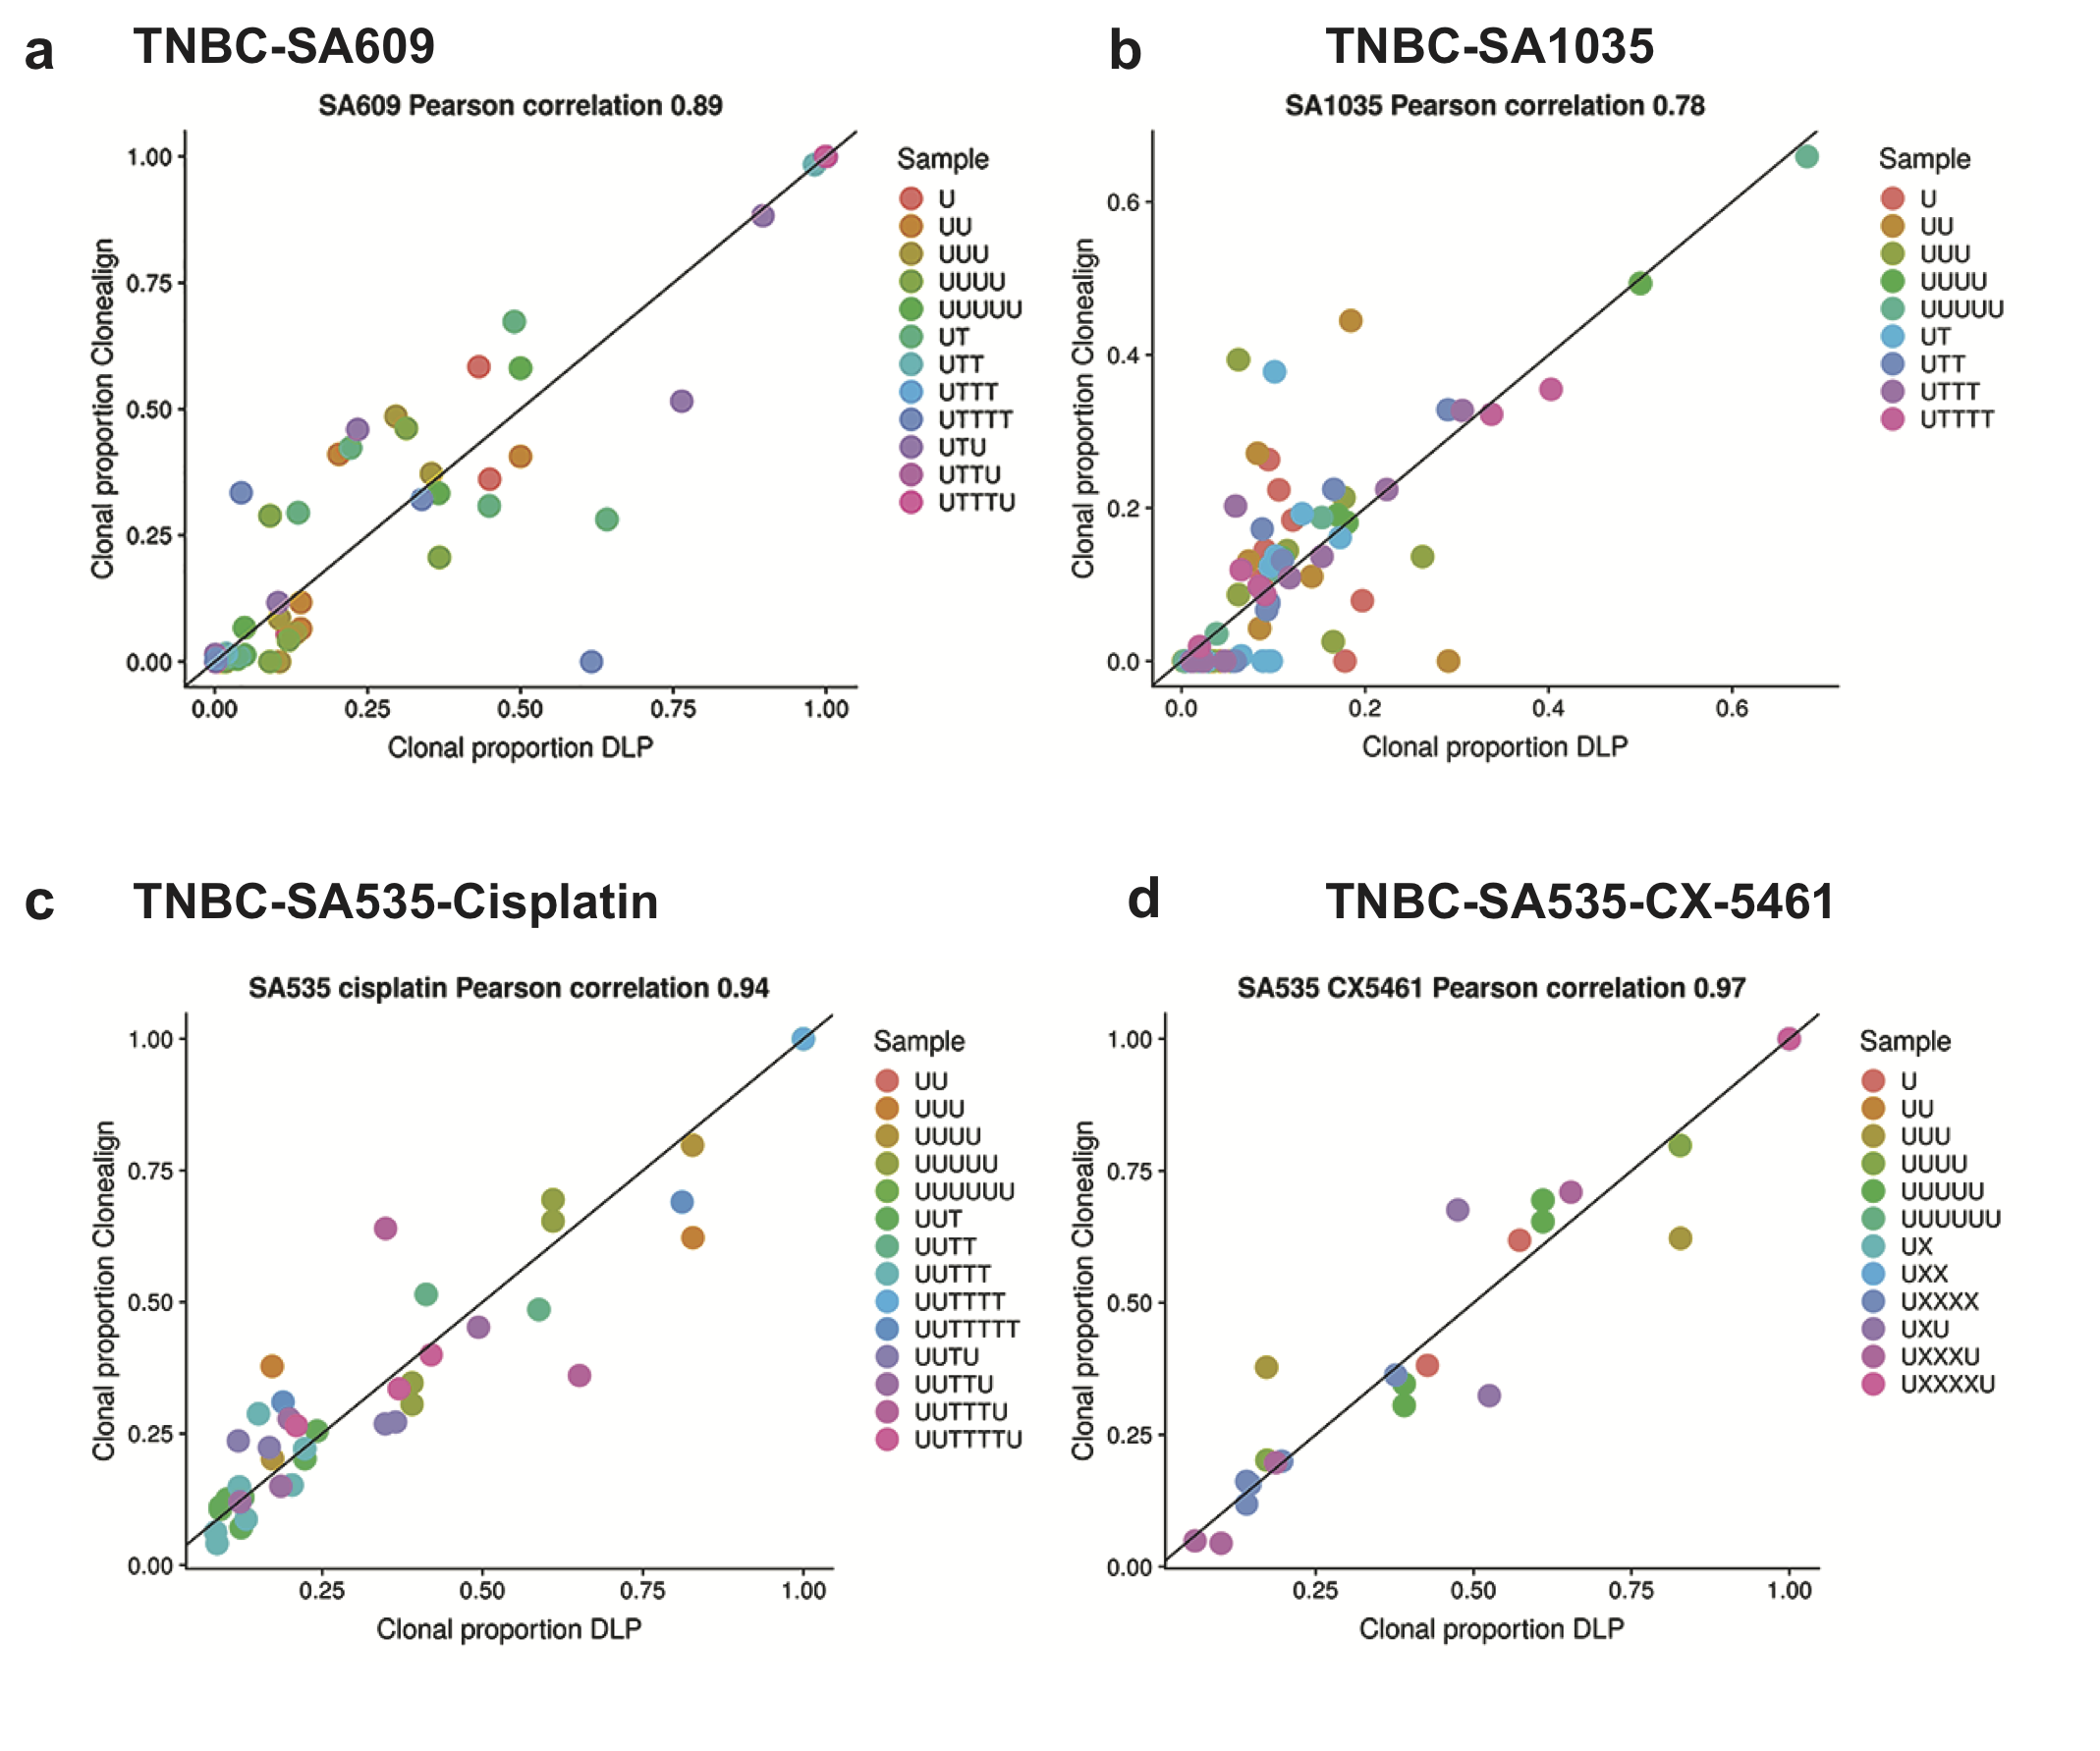
\includegraphics[width=\textwidth]{Figures/chap5/Clonealigncorrelation.png}
	
\caption[\texttt{clonealign} clonal proportions vs DLP+ clonal proportions]
	{\small
	\textbf{\texttt{clonealign}, clonal proportions vs DLP+ clonal proportions.}
	   Clonal proportions of scRNAseq  derived from \texttt{clonealign} estimates (Vertical axis) against proportion of scDNA-seq (DLP+) CNA defined clones (horizontal axis). Number of `T' indicates number of cycles of cisplatin while number of `X' indicates number of cycles of CX-5461.
	   \textbf{(a)} \texttt{clonealign} clonal proportions vs DLP+ clonal proportions of TNBC-SA609 PDX timeseries samples.
	   %indicating positive correlation (Pearson correlation from $r \geq 0.89$).
	 \textbf{(b)} Same as \textbf{(a)} but for TNBC-SA1035 PDX 
	 %and Pearson correlation is $r \geq 0.78$.
	 \textbf{(c)} Same as \textbf{a} but for TNBC-SA535 PDX 
	 %and Pearson correlation is $r \geq 0.94$ for cisplatin treated.
	 \textbf{(d)} Same as \textbf{a}
	 but for SA535 PDX 
	 %and Pearson correlation is $r \geq 0.97$ with CX-5461 treated.
	}
	 
	\label{fig:Clonealigncorrelation}
\end{figure}



%--------------------------------------------------------------------


\begin{figure}
\centering
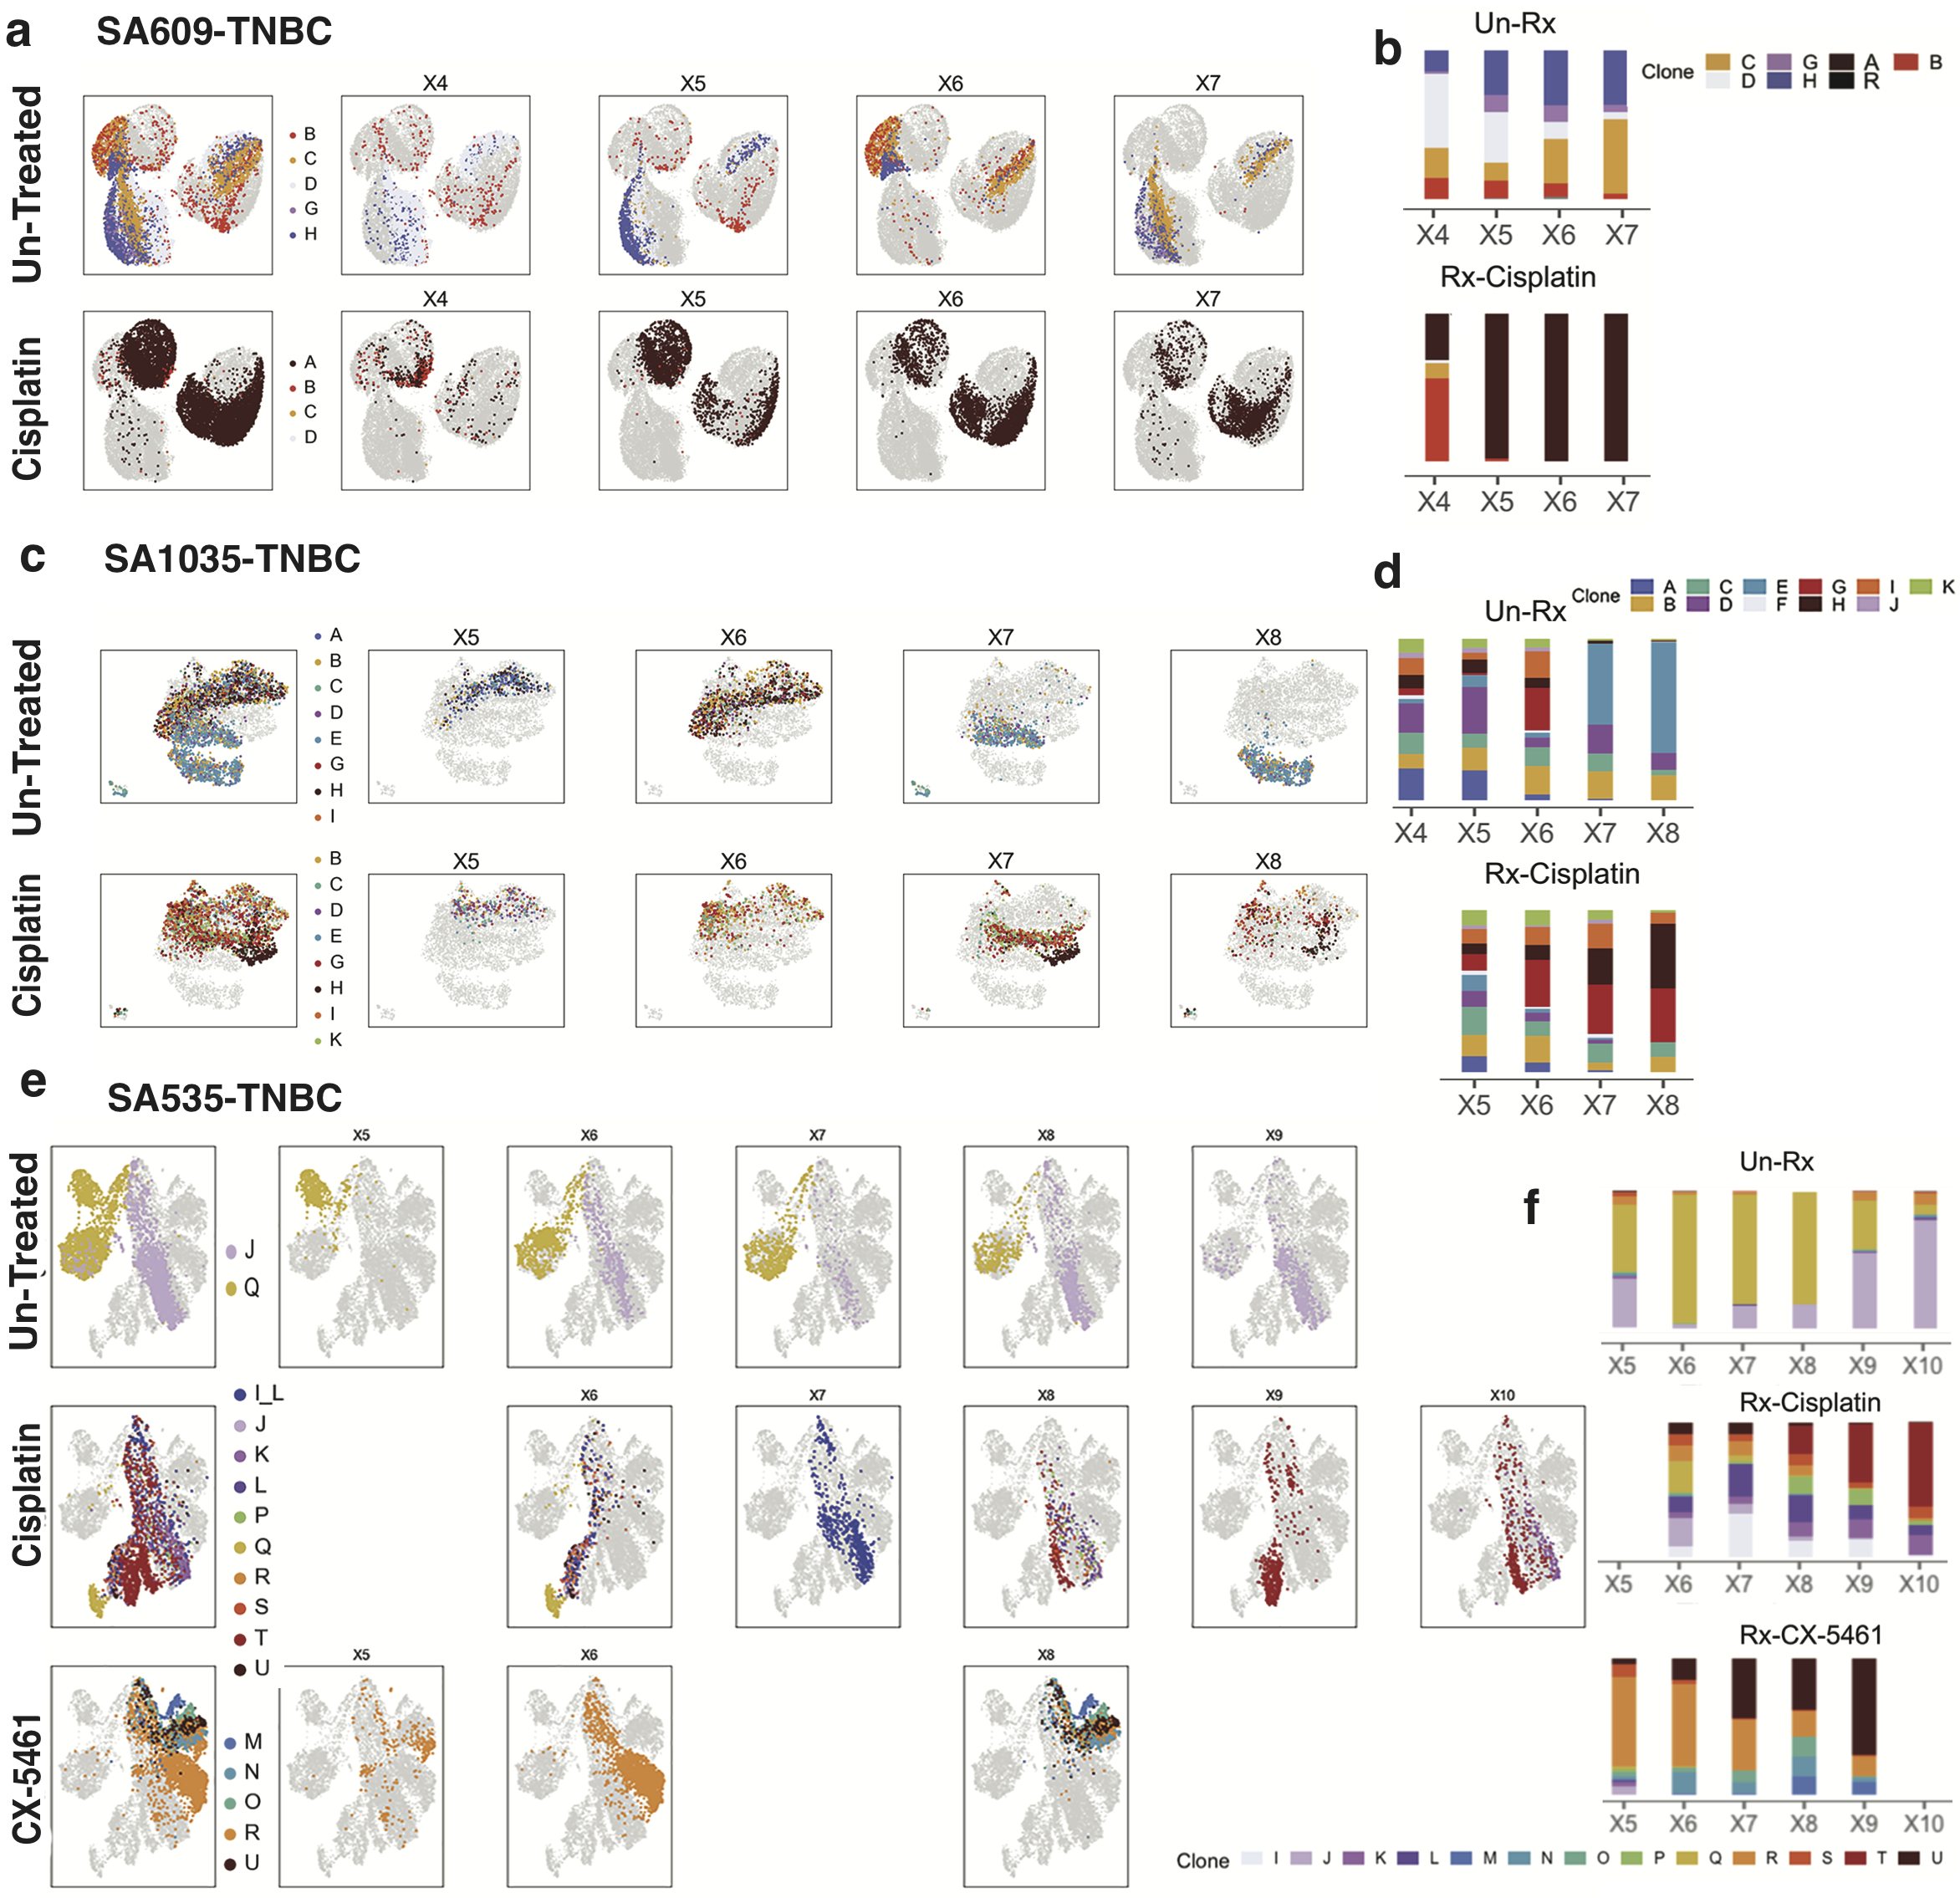
\includegraphics[width=\textwidth]{Figures/chap5/EmbeddingsRNA.png}
	
\caption[Gene expression impacts of clone-specific copy number profiles]
	{\small
	\textbf{Gene expression impacts of clone-specific copy number profiles.}
	    \textbf{(a)} Low dimensional \ac{UMAP} embeddings of matching scRNAseq libraries across the SA609 TNBC timeseries.Top, left and bottom panels show untreated and treated all timepoints embedding annotated with clonealign assignments and right all panels show the density of cell clusters individually over each timeseries X4-X7.
	     \textbf{(b)} Barplots to recall clonal proportion from DLP+ of TNBC-SA609 taken from previous chapter with and without drug. 
	     \textbf{(d)} Same as \textbf{(b)} but for TNBC-SA1035 PDX. \textbf{(e)} Same as \textbf{(a)} but for TNBC-SA535  from X5-X8. \textbf{(f)} Same as\textbf{c} but for SA1035. 
	}
	\label{fig:EmbeddingsRNA}
\end{figure}

%----------------------------------------------------------------


\subsubsection{Normalization and batch correction of scRNA-seq}
%{SCTransform performs more optimal normalization for Single cell RNAseq data in longitudinal \textit{in vivo} experiments}
 %To discern the nature of single cell RNA sequencing data in longitudinal samples, we applied few comparative and diagnostic statistical tools to check the normalization and its effects in our datasets.
The tumor samples of scRNA-seq were collected at different time points because of the nature of experimental design and it was also noted above that large sample variation occurs, suggesting the need for normalization. 
 %Errors in normalization can have a significant impact on downstream analysis, such as high false positives in differential expression analysis.
  To examine this issue, we analyzed the variance between samples of 362 to 512 house keeping genes (HK) that expressed in our dataset  HK were identified from the literature as suitable index genes for batch corrections \cite{lin2019evaluating}, tailed selection criteria is mentioned in methods.
As HK genes can also be influenced by treatments, so we conducted a similar analysis with low variance genes and observed similar results.
\textbf{\autoref{fig:Comparisonofbatcheffects} b} shows high variance (Interquantile ratio range from 0 to 0.86, median 0.13 to 0.94) across HK genes.
we compared the raw data (\textbf{\autoref{fig:Comparisonofbatcheffects} a}) with Seurat \cite{butler2018integrating}, scran \cite{lun2016pooling} and SCTransform \cite{hafemeister2019normalization}. 

We assumed that normalization method with good performance should display stable level of normalized HK genes expression with low variance across libraries.

\textbf{\autoref{fig:Comparisonofbatcheffects} } showed that  \textbf{SCTransform} (median range in all TNBC PDX from 0.1-0.41) and \textbf{Scran} both (median range of 0.21 to 0.66) demonstrated low variance between batches, while sample size effect was observed in \textbf{Seurat} output.

Normalization with SCTransform partially removed batch effects with small range of mean gene expression differences \textbf{\autoref{fig:Comparisonofbatcheffects} a-d}.
 
%Based on series of TNBC-SA1035, SCTransform seems work better than Scran, so  
%Scran: median range: [0.29-0.5]   interquartile: [0.12-0.22]    SCTransform: median range: [0.13-0.26]   interquartile: [0.09-0.17] 
 

\subsubsection{Comparison of \texttt{edgeR} with SCTransform normalization for downstream data analysis}
Here, we set to examine a correlation between raw values, scTransform values and edgeR values for differential gene expression. We anticipated that edgeR differential expression is reasonably correlated to post SCTransform at the same gene loci.

A benchmark study evaluated eleven methods \cite{soneson2013comparison} for differential expression analysis of RNA-seq transcriptomic data, and showed that \texttt{edgeR} outperforms other methods in differential expression estimation with high accuracy of differential expressed genes detection while showing low false discovery rated compared to other methods. As \texttt{edgeR} performs internal normalization, accepting raw data values as input, we sought to evaluate whether differentially expressed (DE) genes that are detected by \texttt{edgeR} are correlated with SCTransform normalization.

It was observed that \texttt{edgeR} and SCTransform normalization were strongly correlated in all timeseries datasets. The correlation coefficients range from 0.78 to 0.9 with the highest correlation in TNBC-SA609 dataset  \textbf{\autoref{fig:edgeRsctransformcorrelation} a}, followed by TNBC-SA1035 with correlation coefficient of 0.8 then TNBC-SA535-CX-5461 with correlation coefficient of 0.79  \textbf{\autoref{fig:edgeRsctransformcorrelation} b, d} and the minimum correlation coefficient was observed in the data of TNBC-535-Cisplatin treated with  0.78 \textbf{\autoref{fig:edgeRsctransformcorrelation} b, d}.



%-----------------------------------------------------------------


%\subsection{Clone-specific genotypes underpin clone-specific gene expression programs}
% where to put this paragraph?
%Next, we profiled the impact of clone specific gene expression changes as a higher order representation of phenotypic properties. We tested if the genotypes of high fitness clones exhibited changes in their transcriptional program, with scRNAseq performed on matched aliquots of same samples sequenced using DLP+ on the serially passaged TNBC PDX as mentioned previously (\textbf{\autoref{fig:RNAsampletree}}.

\subsubsection{Relative abundance of copy number assigned scRNA-seq clonal subpopulations were strongly correlated}
 
 To assess the correlation of DLP+ defined clonal fractions (chapter 4) at each time poinqt in single cell RNA space, we applied \texttt{clonealign}, a statistical method, \cite{campbell2019clonealign} to make a probabilistic assignment of scRNA-seq transcriptomes to copy number determine clones, under the assumption that copy number alterations will also alter transcript levels. It requires prior knowledge of CNA clone genotypes.
 We observed that the relative abundance of clonealign assigned clone memberships for 10x data were well correlated with the previously observed clonal fractions of CNA determined clones \textbf{(\autoref{fig:Clonealigncorrelation}}). TNBC-SA535 treated with CX-5461, (12 libraries), presented the highest confidence correlation with Pearson correlation of 0.97 (p-value$< 10^{-15}$), followed by its cisplatin treated branch (14 libraries), presenting a Pearson correlation of 0.94 (p-value$< 10^{-18}$) \textbf{\autoref{fig:Clonealigncorrelation} c, d}. However, TNBC-SA609 PDX timeseries, (12 libraries) presented a Pearson correlation coefficient of 0.89 (p-value $< 10^{-16}$) \textbf{(\autoref{fig:Clonealigncorrelation} a)} while TNBC-SA1035 , (9 libraries), exhibited the lowest, value of Pearson correlation of 0.78 (p-value$< 10^{-18}$) among all four series \textbf{(\autoref{fig:Clonealigncorrelation} b)}.
  
  
\subsubsection{Single cell copy number clonal structure observed in UMAP summarized transcriptomes with residual batch effects}

The observed clonealign transcriptome correlations suggested that CNA differences between clones may account for some of the phenotypes. To further illustrate this relationship, we summarized the transcriptomes of cells using UMAP dimensional reduction \cite{becht2019dimensionality}, with the clonal assignments of cells shown as embeddings. 

 We found that scRNAseq embeddings displayed a dynamic pattern of global expression over time with and without treatment, which tracked with clone assignments indicating co-variation of transcriptional properties with clonal abundance. UMAP visualization of clusters identified Clone H cells clusters together at the last time point along with Clone C, in untreated setting and Clone A cells clusters together \textbf{\autoref{fig:EmbeddingsRNA} a}, in the cisplatin treated series of TNBC-SA609 PDX, purified over time matching their genomically defined counterparts \textbf{(\autoref{fig:EmbeddingsRNA} b)}. Similarly, Clone E in untreated and Clone H in treated timeseries of TNBC-SA1035  \textbf{(\autoref{fig:Clonealigncorrelation} c)}, clustered uniquely at the later time points. \textbf{\autoref{fig:EmbeddingsRNA} d} reminding the clonal prorportions at each time point in DLP+ emerging with and without treatment from chapter 4 in TNBC-SA1035. 

TNBC-SA535 PDX all three arms of untreated, treated with cisplatin and treated CX-5461, exhibited aggregation of similar patterns of cell clusters that favours emerging of genomic clones in their respective series \textbf{\autoref{fig:EmbeddingsRNA} e, f}. Clone J (purple), in untreated control timeseries \textbf{(\autoref{fig:EmbeddingsRNA} e, top panel)}, Clone T (red), in cisplatin treated \textbf{(\autoref{fig:EmbeddingsRNA} e, middle panel)}, and clone U (dark brown) in CX-5461 treated \textbf{(\autoref{fig:EmbeddingsRNA} e, lower panel)}. They exhibited approximately similar proportions with respect to other clones as observed in DLP+ (\textbf{\autoref{fig:EmbeddingsRNA} f}). 

Furthermore, some batch effects could be seen more obvious in TNBC-SA1035, X7 to X8, even after normalization and batch correction (\textbf{\autoref{fig:EmbeddingsRNA} c}). The major clone E (blue) along with minors, B and D, are clustering in two different dimensions in untreated passage X7 and passage X8. However, they are clustering together indicating that although there are some residual batch effects showing up but the cells belong to the same group.

%------------------------------------------------------------------

\begin{figure}
\centering
  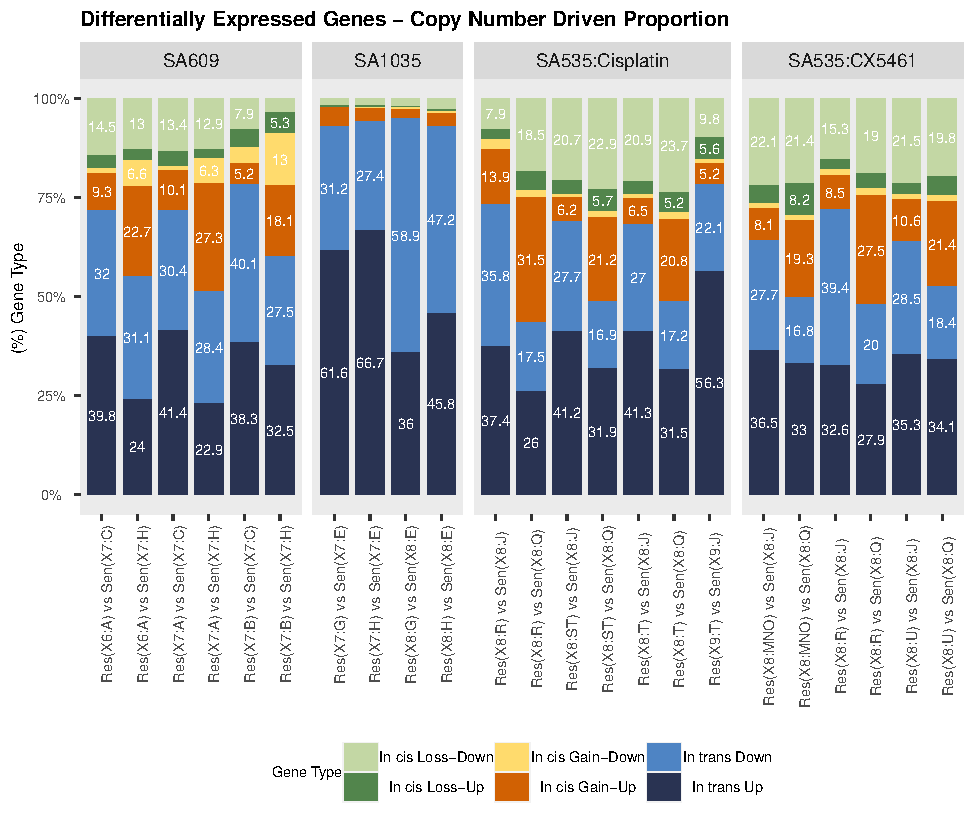
\includegraphics[width=\textwidth]{Figures/chap5/fig4Summaryincistrans.pdf}
	
\caption[Summary proportion of \textit{in cis} and \textit{in trans} regulated gene expression in scRNAseq data]
	{\small
	\textbf{Proportion of CNA differences mapping to resistant and sensitive clone differentially expressed genes.}
	  Vertical axis represents the percentage of DE genes. Horizontal axis represents the two clones. The numbers written for each coloured bar represent the percentage of respective category between those two clones.
	     
	}
	\label{fig:fig3Summaryincistrans}
\end{figure}

%---------------------------------------------------------------

\subsection{Contrasts of resistant and sensitive clone specific gene expression reveals the rates of \textit{in cis} and \textit{in trans} components}
The above analysis points to copy number mediated effects on transcriptome phenotype, thus we set out to estimate the proportion of the transcriptome affected \textit{in cis} versus that affected \textit{in trans}. 

We intersected differentially expressed genes (DE) by comparing resistant clones from all the 4 treated timeseries PDX versus sensitive clones of all the timeseries PDX. A  (DE) is \textit{in cis} regulated if there was a difference in median copy number for that gene between the two compared clones, and \textit{in trans}, if the median copy number remains the same but the gene is differentially expressed between resistant and sensitive clones (either upregulated or downregulated). \textbf{{\textit{in cis} positive tendency}} means if the gene expression is up regulated with the gain in copy number, whereas, \textbf{{\textit{in cis} negative tendency}} means that the gene expression is paradoxically changing with change in copy number. However, \textbf{\textit{in trans}} genes are independent of copy number change.

To determine how much of the transcriptome is modulated by \textit{in cis} and \text{in trans}, first, we identified sensitive and resistant clones from the DLP+ clones summarized in chapter 4. We assumed that the clones that showed fitness advantage under drug selection were resistant because they were high abundance clones (tumor growth inhibition was low in those tumors), whereas the clones that had high fitness coefficients in the absence of drug were sensitive because they could not survive under drug pressure but showed fitness advantage over others in the absence of drug (\textbf{\autoref{tab:Listofresistantandsensitiveclones}}). We focused on differential expression analysis of these major resistant and sensitive clones to simplify the analysis.

\subsubsection{Copy number change \textit{in cis} expression accounts for {$\sim${~}}5.2\% and 56.5\% of clonal differences in resistant vs sensitive transcriptomes}

We next investigated the proportion of the genome in resistant and sensitive clones that is potentially influenced by clone copy number differences (cis regulation) and that which was outside of observed copy number differences (trans regulation) as defined above.

Some of the selected clones that were closely related to the resistant clones or having second highest fitness coefficients in DLP+ data from chapter 4, were also added to DE analysis from each of the time series PDX using \texttt{edgeR}. For example, clone R was not a resistant clone but it gave rise to two different resistant clones under different drugs and clone Q stayed in high abundance in earlier untreated passages of SA535.

Using \texttt{edgeR} determined differential expression, we classifed genes into cis and trans up or down regulated, according to the overlap with clone specific copy number differences, or common genomic regions. \textbf{\autoref{fig:fig3Summaryincistrans} a}.

We identified overlapping positions between chromosome segments and known genes, then we assigned those segments to an ensemble gene ID \cite{rainer2019ensembldb} of the  selected \ac{DE} of clones across all timeseries and calculated their number and percentages in each PDX timeseries. Notably, we found that the overall number of \textit{in trans} genes were higher as compared to \textit{in cis}, which is supporting previously reported results \cite{shao2019copy}. 


Furthermore, it was found that \textbf{SA535:Cisplatin} had the highest percentage of \textit{in cis} genes with average of 41.7 (SD:9.67) followed by  and \textbf{SA535:CX-5461} with average of 38.57 (SD:14.0), \textbf{SA609} with average of 35.27 (SD:10.79)the lowest percenatge of \textit{in cis} genes were observed in \textbf{SA1035} with average of 6.3 (SD:0.92).

Among differentially expressed genes between resistant and sensitive clones, \textit{in cis} \textbf{upregulated} transcripts associated with CNA gain in resistant clone, varied between 2.3\% in SA1035 to 31.5\% in SA535:cisplatin. In contrast, \textit{in cis} \textbf{downregulated} transcripts associated with CNA gain in resistant clone, varied between 0.1\% in SA1035 and 13\% in SA535 cisplatin. However, proportion of \textit{in trans} genes varied between 43.5\% and 94.9\% across all PDX series with highest in \textbf{SA1035} with percentage of \textit{in trans} genes with average of 93.7 (SD:0.98).


%------------------------------------------------------
% Table generated by Excel2LaTeX from sheet 'Sheet1'
 \begin{table}[htbp]
   
   \centering
   \caption{List of resistant and sensitive clones across TNBC PDX}
     \begin{tabular}{|l|l|l|}
      \hline
     TNBC PDX & Resistant clone & Sensitive clone \\
     \hline
     TNBC-SA609  & Clone A & Clone H \\
     TNBC-SA1035 & Clone H & Clone E \\
     TNBC-SA535-Cisplatin Rx & Clone S\_T & Clone J \\
     TNBC-SA535-CX-5461 Rx & Clone U & Clone J \\  
     \hline
     \end{tabular}%
   \label{tab:Listofresistantandsensitiveclones}%
   
 \end{table}%
%--------------------------------------------------------------------------

\subsubsection{Proportions of high essentiality genes, cancer drivers and known cisplatin genes reflect the same proportions of \textit{in cis} and \textit{in trans} in our dataset}
Next, we asked what proportion of the \ac{DE} genes (resistant and sensitive clones) intersect with various databases were in \textit{in cis} and \textit{in trans}.

We probed four databases, including data DepMap BroadSanger essential gene set \cite{dempster2019agreement}. COSMIC (catalogue of somatic mutations in cancer) \cite{forbes2010cosmic}, ADAM PanCancer Core cancer fitness  \cite{behan2019prioritization}, and cisplatin related genes curated from recent literature (\textbf{\autoref{tab:Cisplatinrelatedgenes}}).

First, we pulled the reference genes from these databases that were intersecting with our \ac{DE} dataset and calculated if they are regulated with the change in copy number.
Average of proportion of gene set membership over 4 reference gene sets were 10.3\%, 10.44\%, 12.8\% \textit{in cis}, and 16.8\%, 14.02\%, 15\% \textit{in trans} in SA609, SA535-cisplatin, SA535-CX5461, respectively 

Interestingly, we noticed that TNBC-SA535 in both treatment regimes, inferred highest rate of \textit{in cis} genes with 28\% maximum, whereas, TNBC-SA1035 possessing the lowest rate of 2.4\% maximum. TNBC-SA609 showed 12.8\% of its highest \textit{in cis} gene rate \textbf{\autoref{fig:incisgenesindatasets}}.

 Overall, our results remained consistent with the fact that \textit{in cis} and \textit{in trans} representation of DE in various datasets from SA609 and SA535 treated both with cisplatin and CX-5461, were almost balanced but in SA1035, consistent with our previous results showed high average of \textit{in trans} with 22.4\%  and low average of 1.07\% \textit{in cis} \textbf{\autoref{fig:incisgenesindatasets}}.


%Then we extract 983 common essential genes that exist in both list to use as our essentiality genes reference, and map our DE genes results with this reference gene set,
%The summary of number of genes and their percentages in each clone comparison in high cancer essentiality gene list (Broad \& Sanger institute) is given in \textbf{\autoref{tab:Broadsanger}}. 

 %In TNBC-SA609 PDX, the mean number of \textit{in cis} genes was 1173.8 (segment positions, $\sigma$ = 494 \textit{in cis} genes, max= 1640, min=215), TNBC-SA1035 presented with the lowest \textit{in cis} with
 %mean value of 187.8 (segment positions, $\sigma$ = 51 \textit{in cis} genes, max=246, min=144). TNBC-SA535 in cisplatin timeseries showed mean number of 1056.9 \textit{in cis} genes (segment positions, $\sigma$ = 624 , max=1900, min=116), whereas, TNBC-SA535 in CX-5461 exhibit highest number of mean \textit{in cis} value of 1400.7 (segment positions, $\sigma$ = 481 \textit{in cis} genes, max=1884, min=739).
 
  
%----------------------------------------------------------------


\begin{figure}
\centering
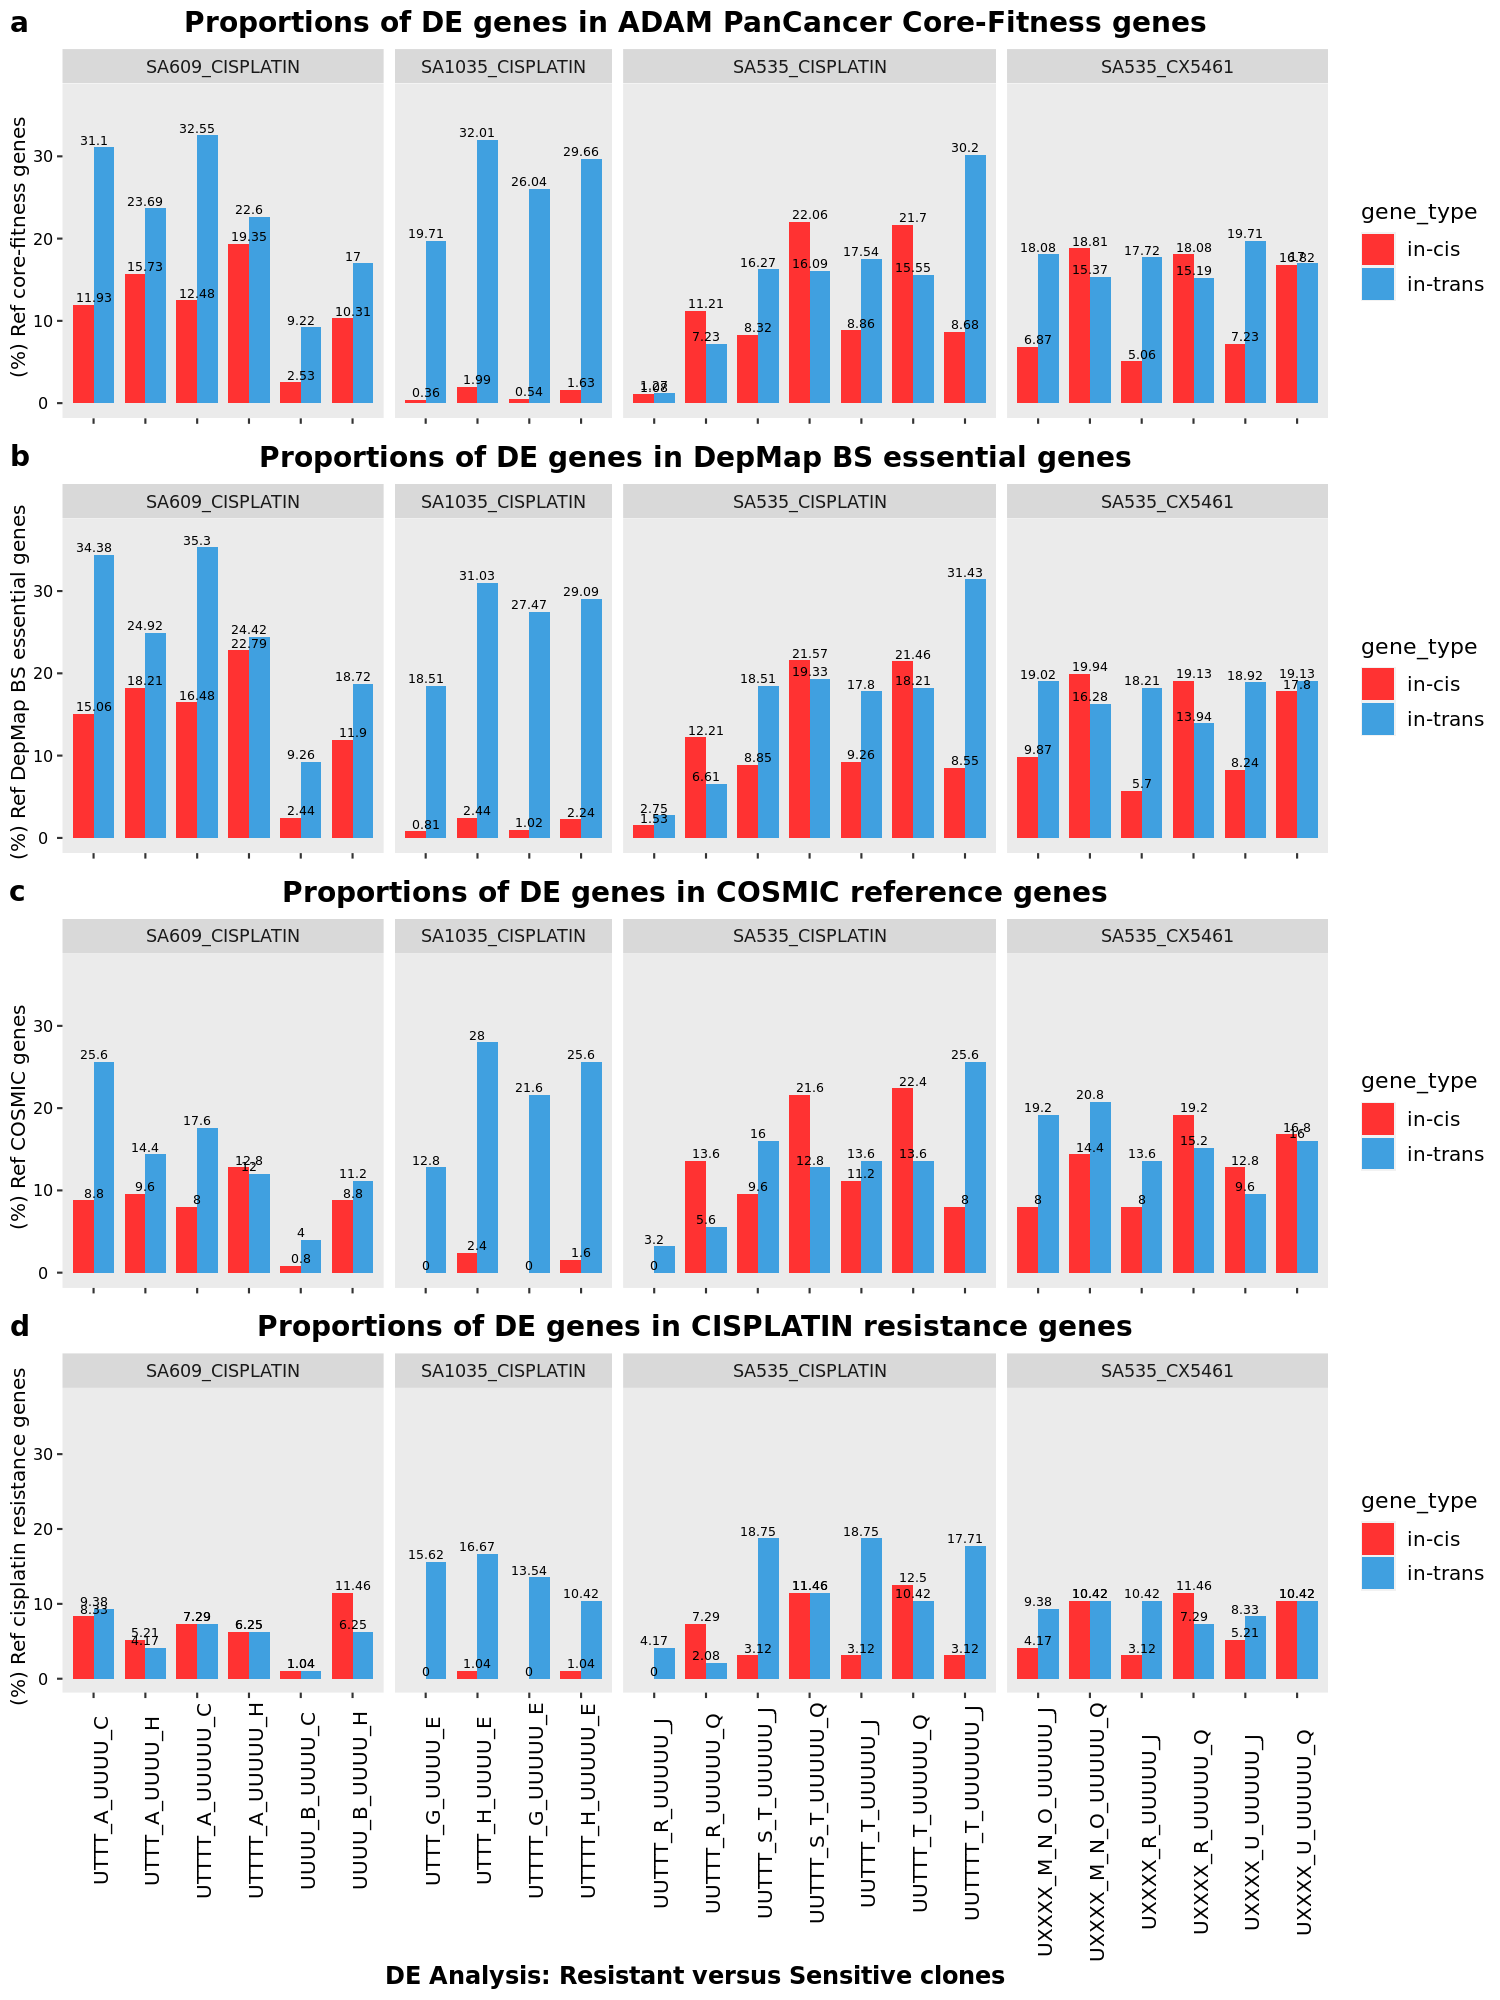
\includegraphics[width=\textwidth]{Figures/chap5/incispercenatgeindatasets.png}

\caption[Summary of number of cisplatin resistance genes \textit{in-cis} and \textit{in-trans}]
	{\small
	\textbf{Mapping \textit{in cis} and \textit{in trans} gene proportions to various datasets.}
	Gene set membership \textit{in cis} and \textit{in trans} differential expression between resistant and sensitive clones 
     \textbf{(a)} Proportions of DE gene in ADAM PanCancer Core fitness dataset \cite{behan2019prioritization}. Percentages are written on each bar where red indicating proportion of \textit{in cis} genes and blue indicates the proportion of \textit{in trans} that are matching with the respective list.
     \textbf{(b)} Analogous to  \textbf{(a)} but the reference dataset is DepMap BroadSanger essential gene set \cite{dempster2019agreement}.
		\textbf{(c)} Analogous to \textbf{(a)} but the reference dataset is COSMIC cancer gene set \cite{forbes2010cosmic}.
		\textbf{(d)} Analogous to \textbf{(a)} but the reference dataset is Cisplatin resistance related geneset (\textbf{\autoref{tab:Cisplatinrelatedgenes}}).

}
    \label{fig:incisgenesindatasets}
    \end{figure}
    
%---------------------------------------------------------------
\subsubsection{Differential expression analysis of resistant and sensitive clones reveals cancer related genes}

To get the magnitude of expression differences of up and down regulated genes between resistant and sensitive clones, we explored \ac{DE} with respect to their regulation \textit{in cis} and \textit{in trans}.

First observation from all the four volcano plots was consistent with the fact that overall the number of \textit{in trans}regulated genes were greater than \textit{in cis} number of genes \textbf{\autoref{fig:Volcanoes4plots}}.


Furthermore, we found that DE \textit{in cis} genes range from 6.9\% (SA1035-resH and senE) to 48.7\% (SA609-resA and senH) of all DE genes, for resistant vs sensitive clones. However, The proportion of DE \textit{in trans} genes range from- 44.12\% (SA609-resA vs senH) to  93.18\% (SA1035-resH and senE) and  72.2\% and  59.26\% for SA535-cisplatin and CX-5461 treated, respectively.

Moreover, In top 5\%, the proportion of \ac{DE} of all datsets of resistant versus sensitive clones, the percentage of \textit{in trans} were higher than \textit{in cis} genes, except for series SA609, where \textit{in trans} almost balance \textit{in cis} with the percentages of 44.12\% and 55.88\% respectively.

Next, we looked into the difference of magnitude between up regulated genes and downregulated \ac{DE} genes. Notably, all comparisons of the resistant versus sensitive clones showed approximately equal upregulated and downregulated gene sets accept for SA535-cisplatin treated resistant and sensitive comparison, that had around double the difference \textbf{\autoref{fig:Volcanoes4plots} c}.

In-cis direction reflected in DE, but minority of genes DE against the direction of copy number gain/loss - refer also to fig 5.10 and 5.11 for this result. (for example myc)



%----------------------------------------------------------------------

\begin{figure}
\centering
  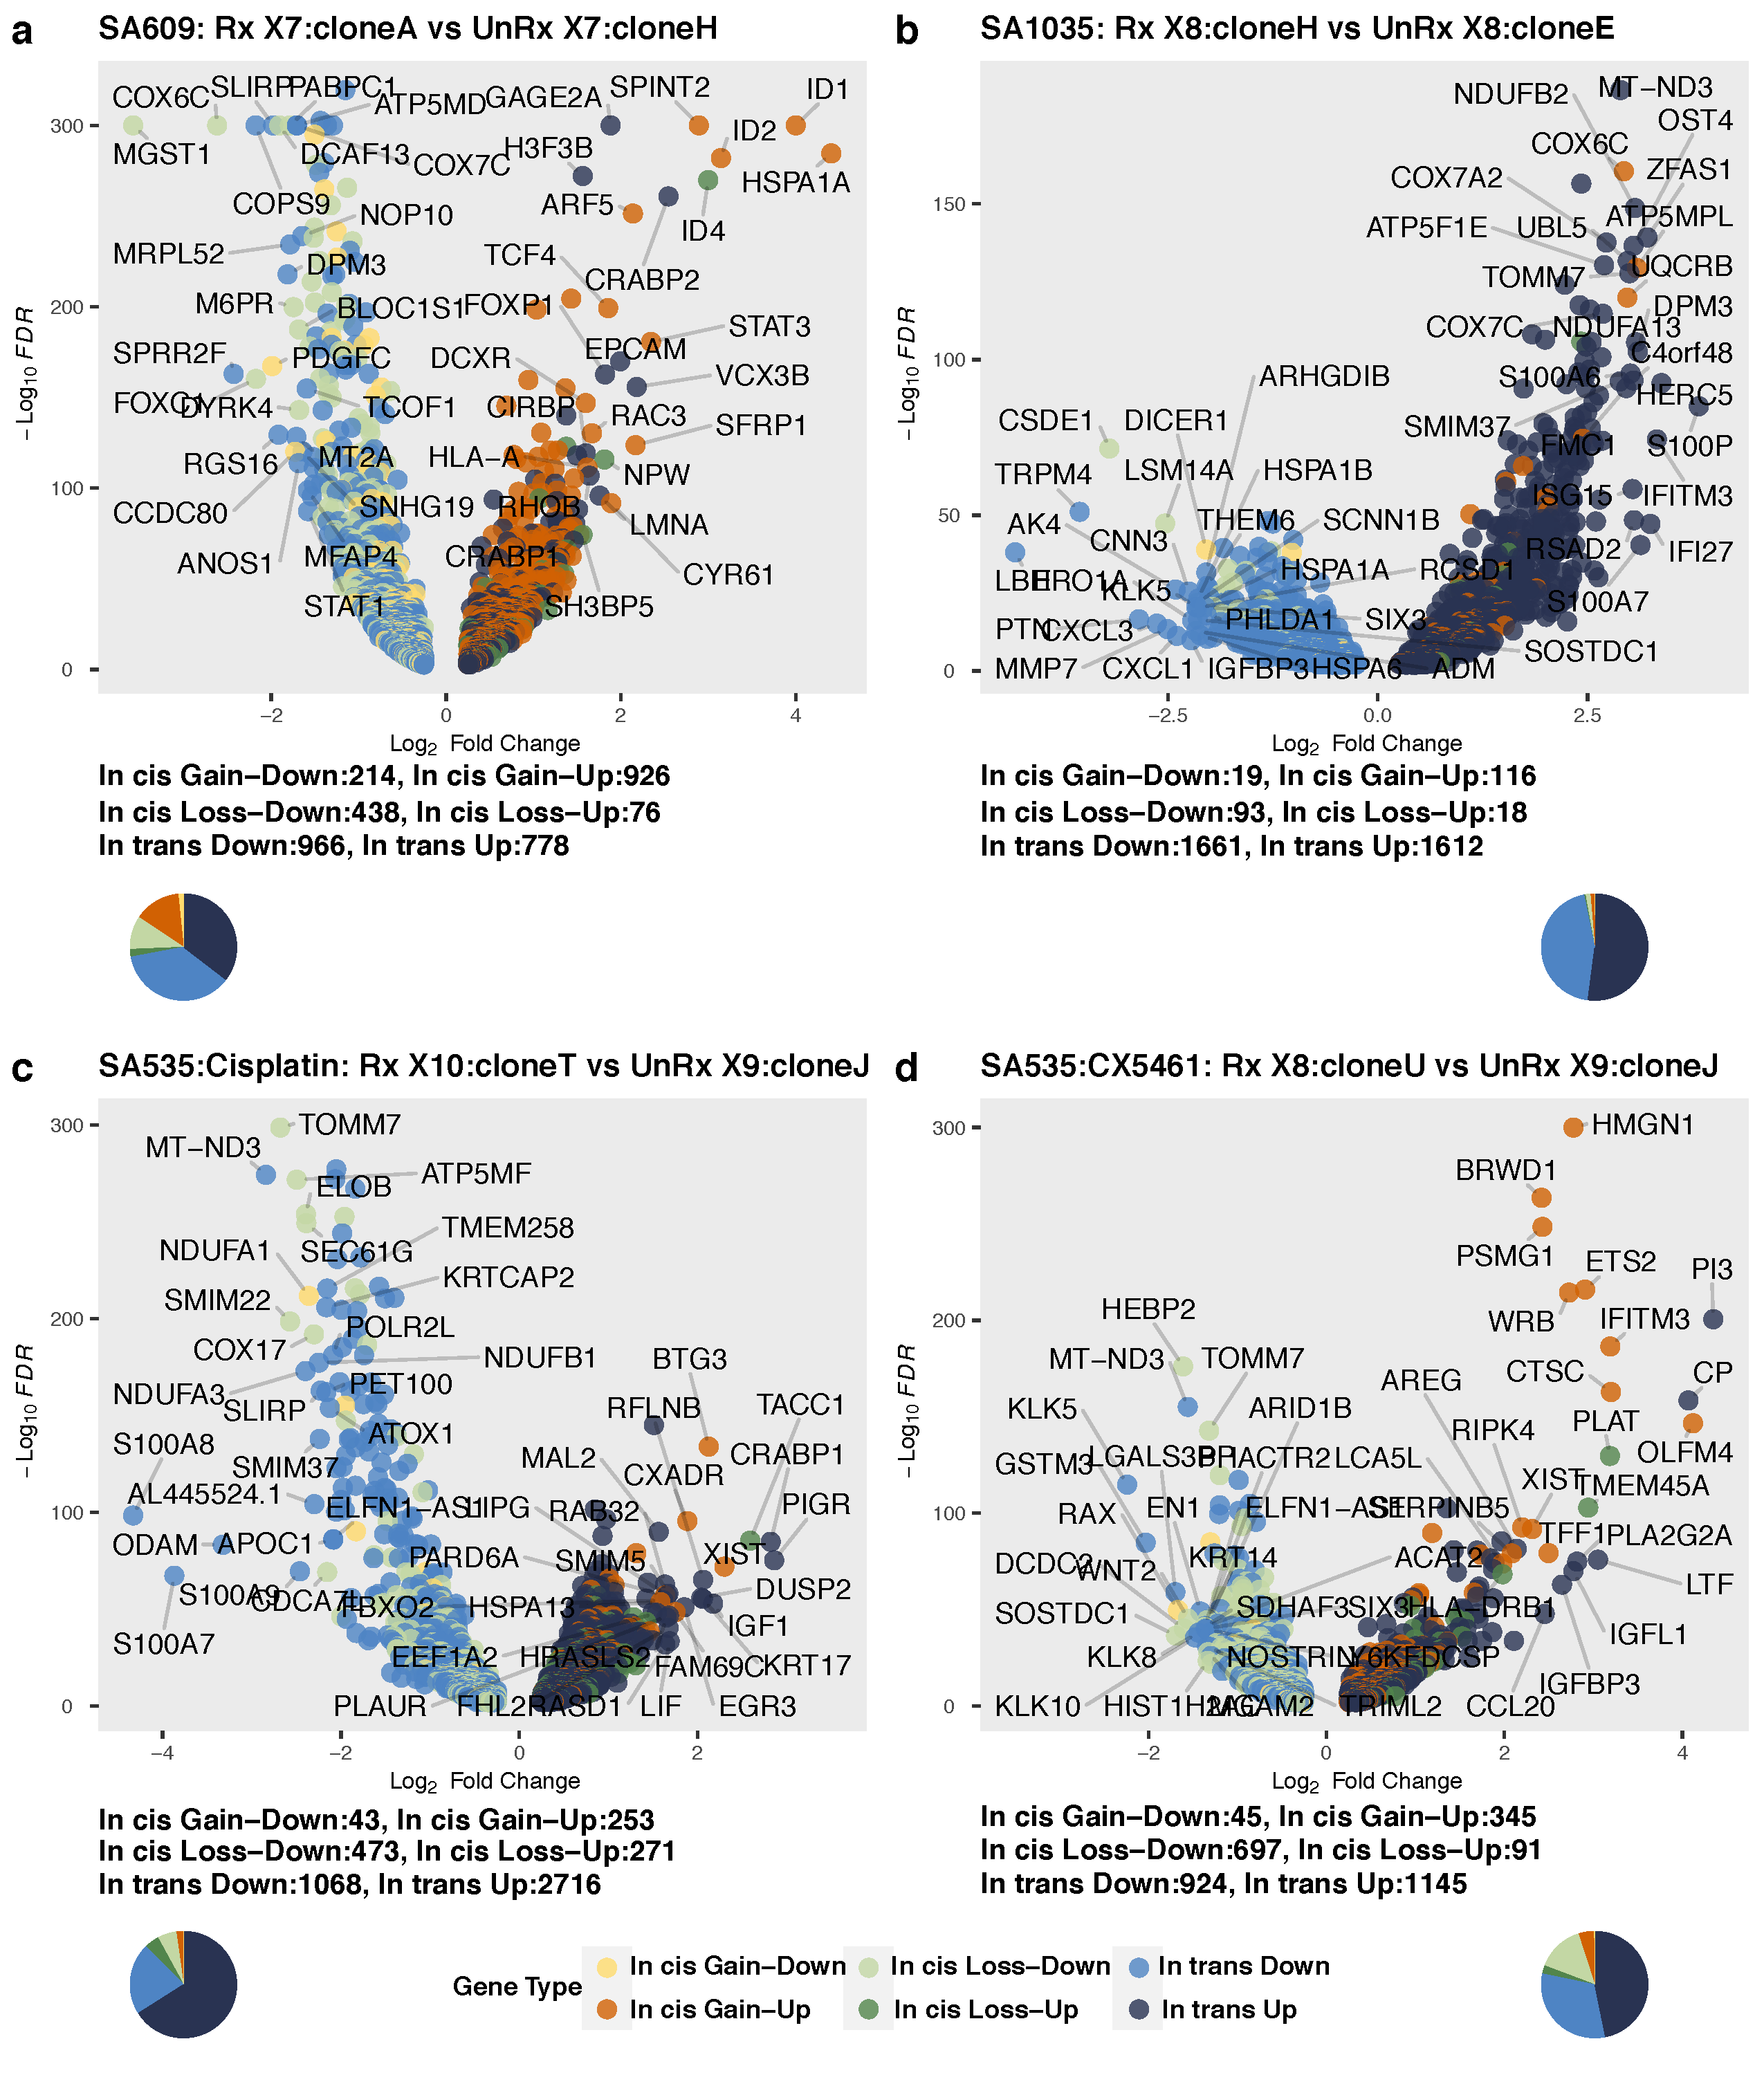
\includegraphics[width=\textwidth]{Figures/chap5/Volcanoes4plots.png}
\caption[DE of resistant and sensitive clonealign defined clones]
	{\small
	\textbf{Differential expression of resistant versus sensitive clones.}
	Horizontal axis shows the logbase 2 fold change values of \texttt{edgeR} differential expression analysis between resistant versus sensitive clones. Vertical axis shows the -log base 10 of false discovery rate (-log10FDR) of ac{DE} genes, colors denote different gene types. 4 pie charts:  proportion of each gene type as in key.
	\textbf{(a)} Volcano plot from SA609 -log10 (FDR) plotted against log2 fold change of pairwise differential gene expression between resistant and sensitive clones. (The threshold for significant genes are FDR p$<$00.01, P Value p$<$00.05, logFC p$>$00.25). \textbf{(b)} Analogous to \textbf{a} but in SA1035. \textbf{(a)} Analogous to \textbf{a} but in SA535-Cisplatin. \textbf{(d)} Analogous to \textbf{a} but in SA535 (CX-5461).
	   }
	\label{fig:Volcanoes4plots}
 \end{figure}

%------------------------------------------------------------

\begin{figure}
\centering
  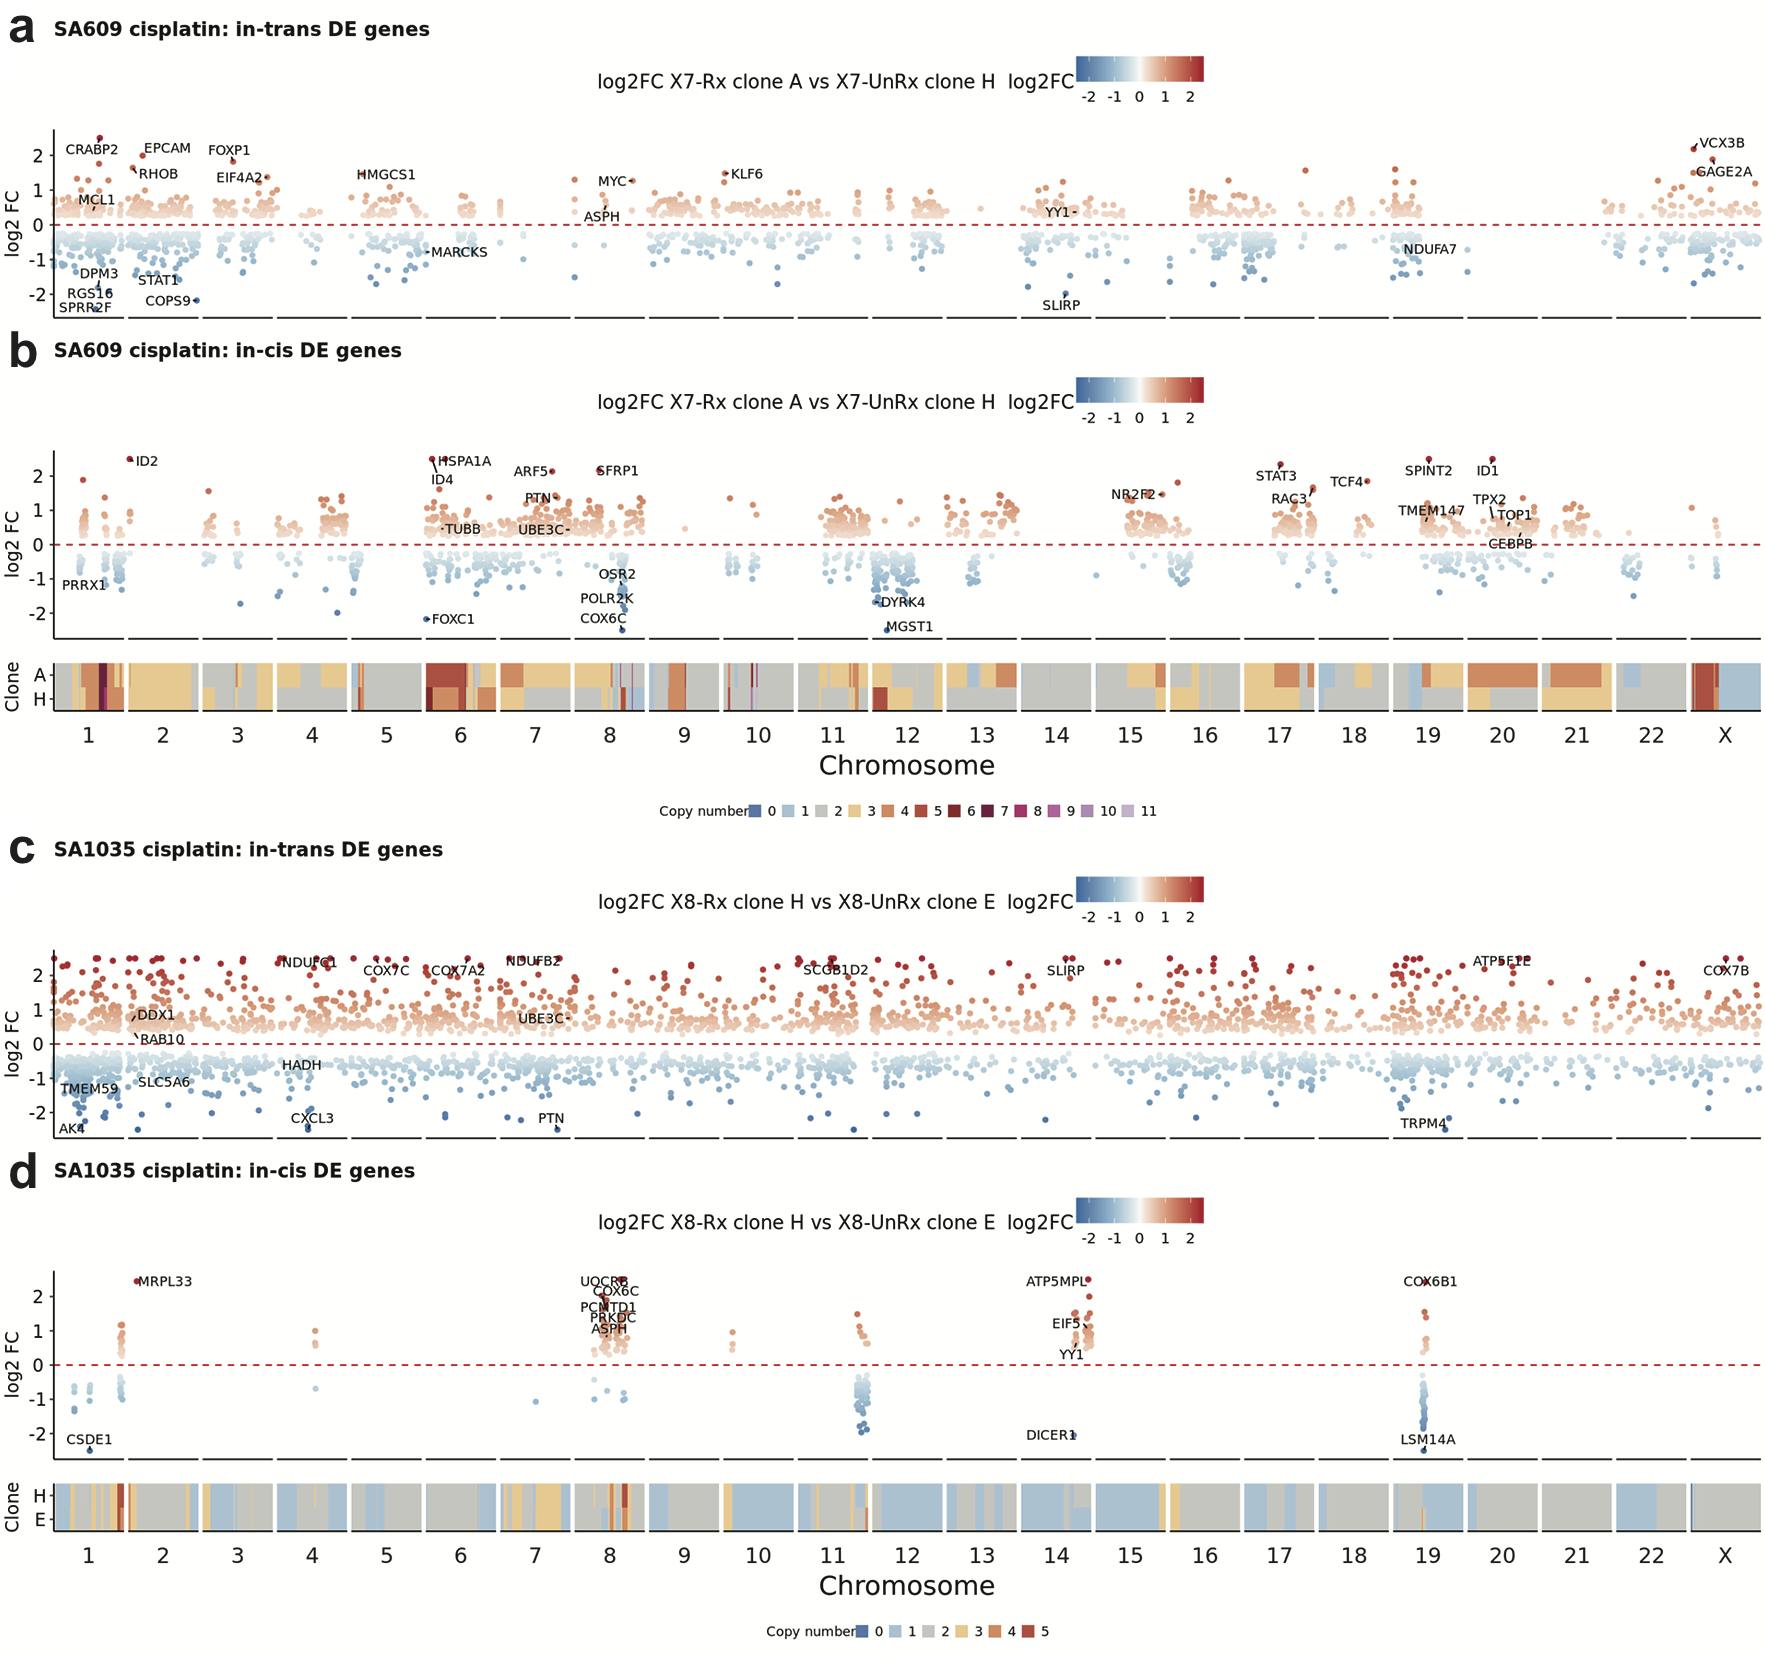
\includegraphics[width=\textwidth]{Figures/chap5/trackplotsSA609SA1035.png}
\caption[DE of resistant and sensitive clonealign defined clones]
	{\small
	\textbf{Differential expression of resistant and sensitive clones in TNBC-SA609 and TNBC-SA1035.}
 In each panel, the upper portion shows $\log 2$ fold change, with red showing higher log fold change in the top clone and blue showing higher log fold change in the bottom clone. The lower portion shows the median copy number of each gene from the DLP+ data, in the rank order of appearance in the genome.  Differential gene expression between the resistant and sensitive clone. The percentage of \textit{in-cis} differentially expressed genes (DEGs) is calculated as having a corresponding change in copy number, out of all the DEGs considered. 
 \textbf{(a)} Upper panel shows Manhattan plots of \textit{in cis} DEG, while bottom panel shows \textit{in trans} in TNBC-SA609.
 \textbf{(b)} Same as \textbf{(a)} but in TNBC-SA1035.
}
	\label{fig:trackplotsSA609SA1035}
 \end{figure}

%------------------------------------------------------------
\begin{figure}
\centering
  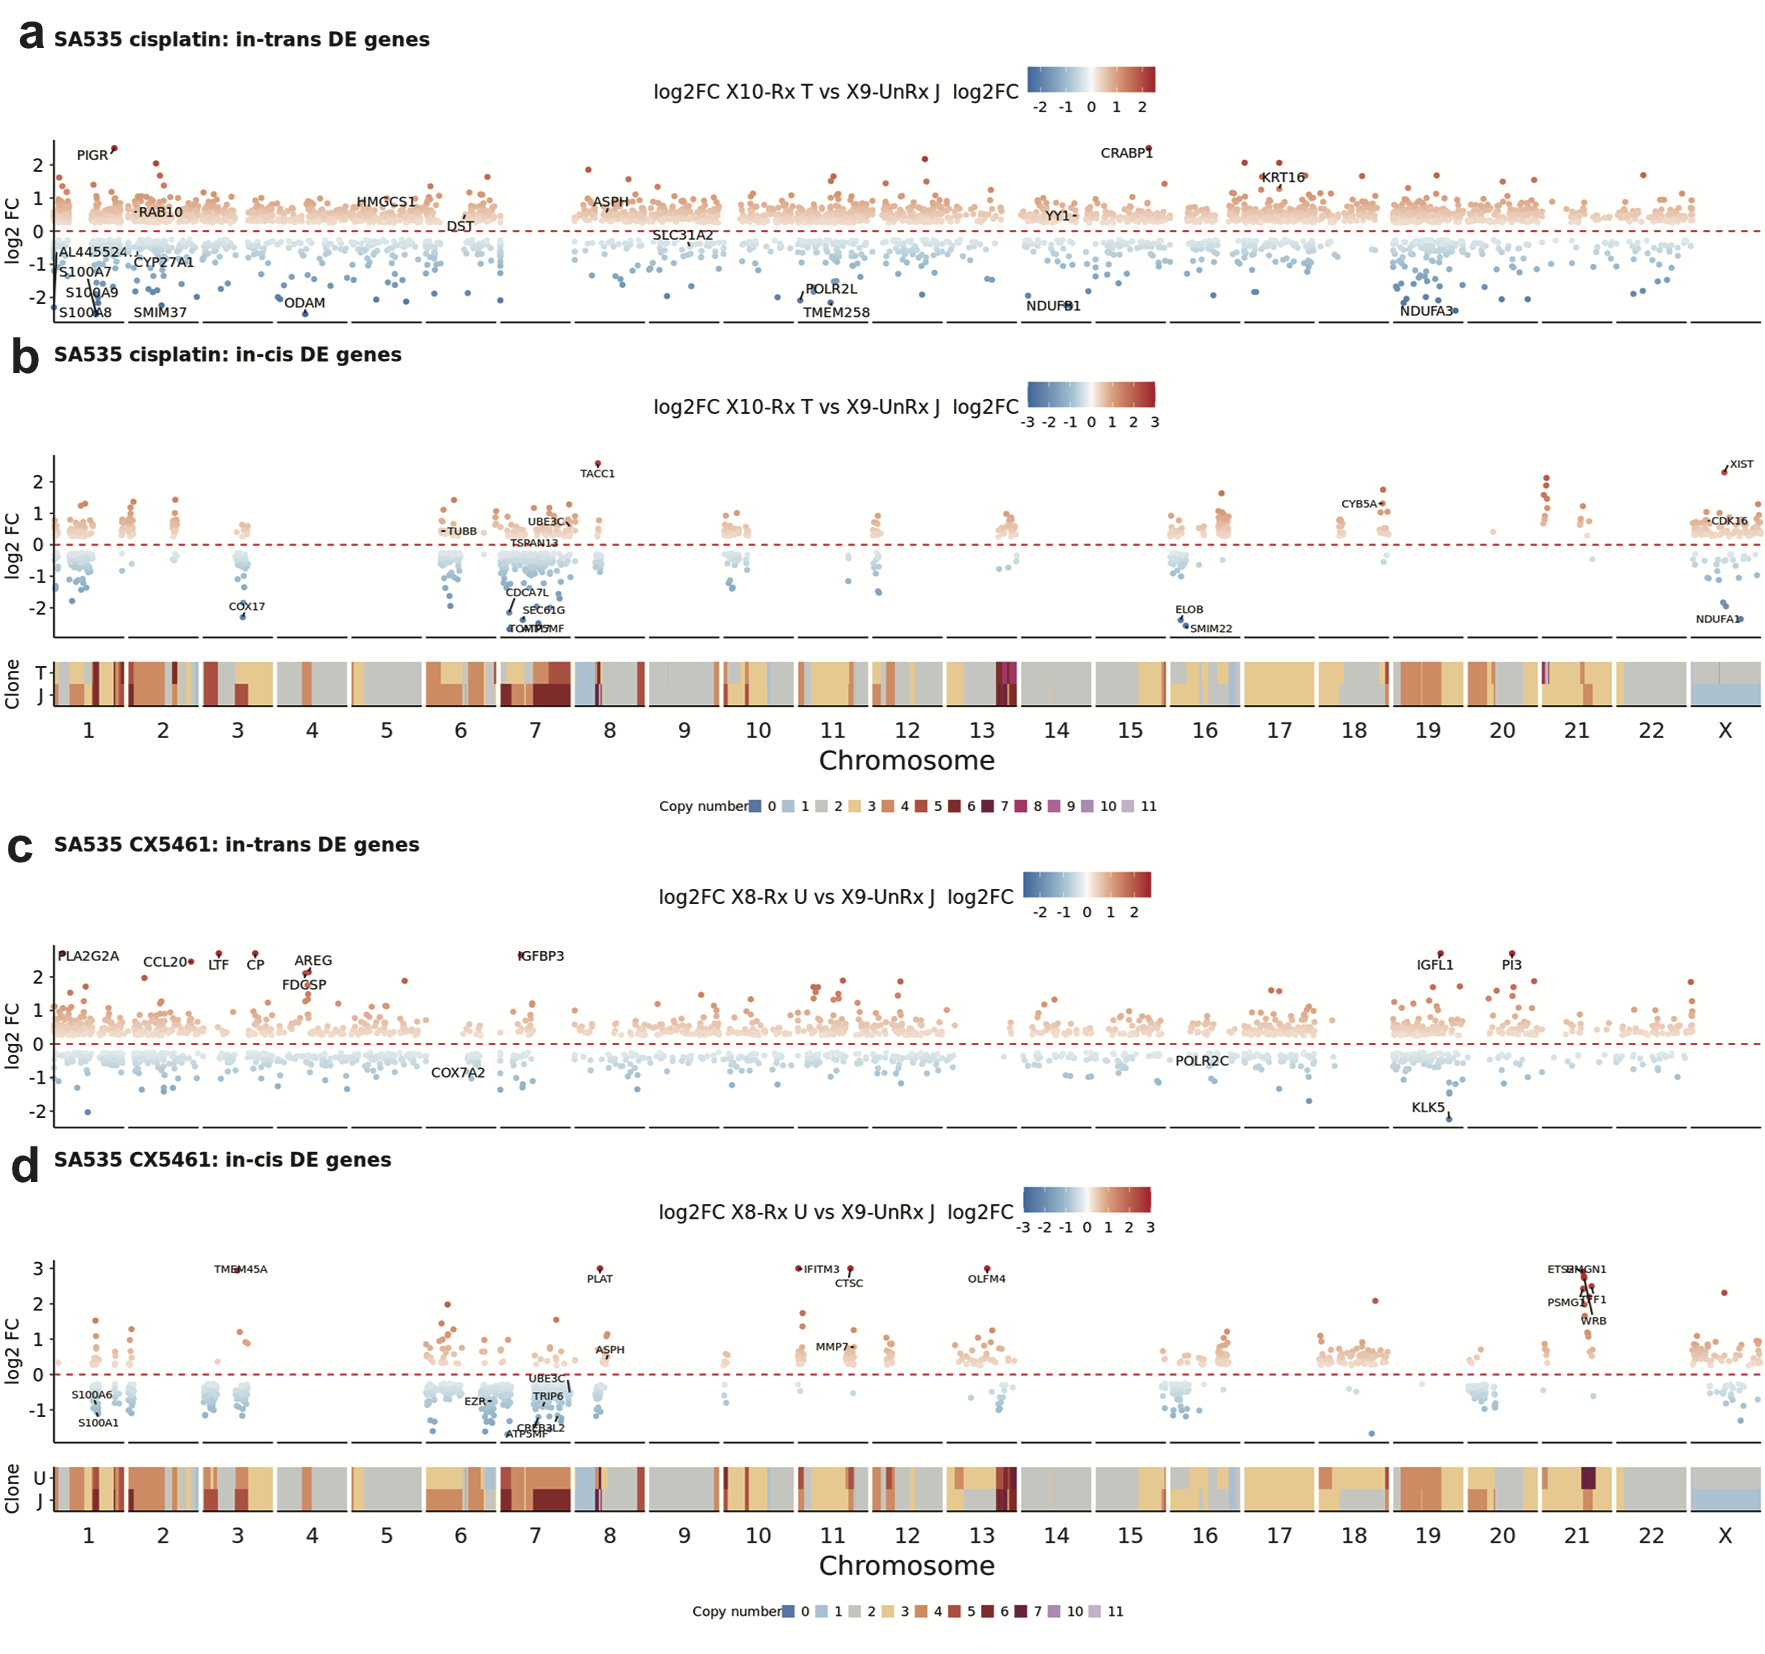
\includegraphics[width=\textwidth]{Figures/chap5/trackplotsSA535.png}
\caption[DE of resistant and sensitive clonealign defined clones]
	{\small
	\textbf{Differential expression of resistant and sensitive clones in TNBC-SA535 treated with cisplatin and CX-5461.}
 In each panel, the upper portion shows $\log 2$ fold change, with red showing higher log fold change in the top clone and blue showing higher log fold change in the bottom clone. The lower portion shows the median copy number of each gene from the DLP+ data, in the rank order of appearance in the genome.  Differential gene expression between the resistant and sensitive clone. The percentage of \textit{in-cis} differentially expressed genes (DEGs) is calculated as having a corresponding change in copy number, out of all the DEGs considered. 
 \textbf{(a)} Upper panel shows Manhattan plots of \textit{in cis} DEG, while bottom panel shows \textit{in trans} in TNBC-SA609.
 \textbf{(b)} Same as  \textbf{(a)} but in TNBC-SA1035.
}
	\label{fig:trackplotsSA535}
 \end{figure}
%------------------------------------------------------------







% Please add the following required packages to your document preamble:


%------------------------------------------------------------
 %\begin{figure}
%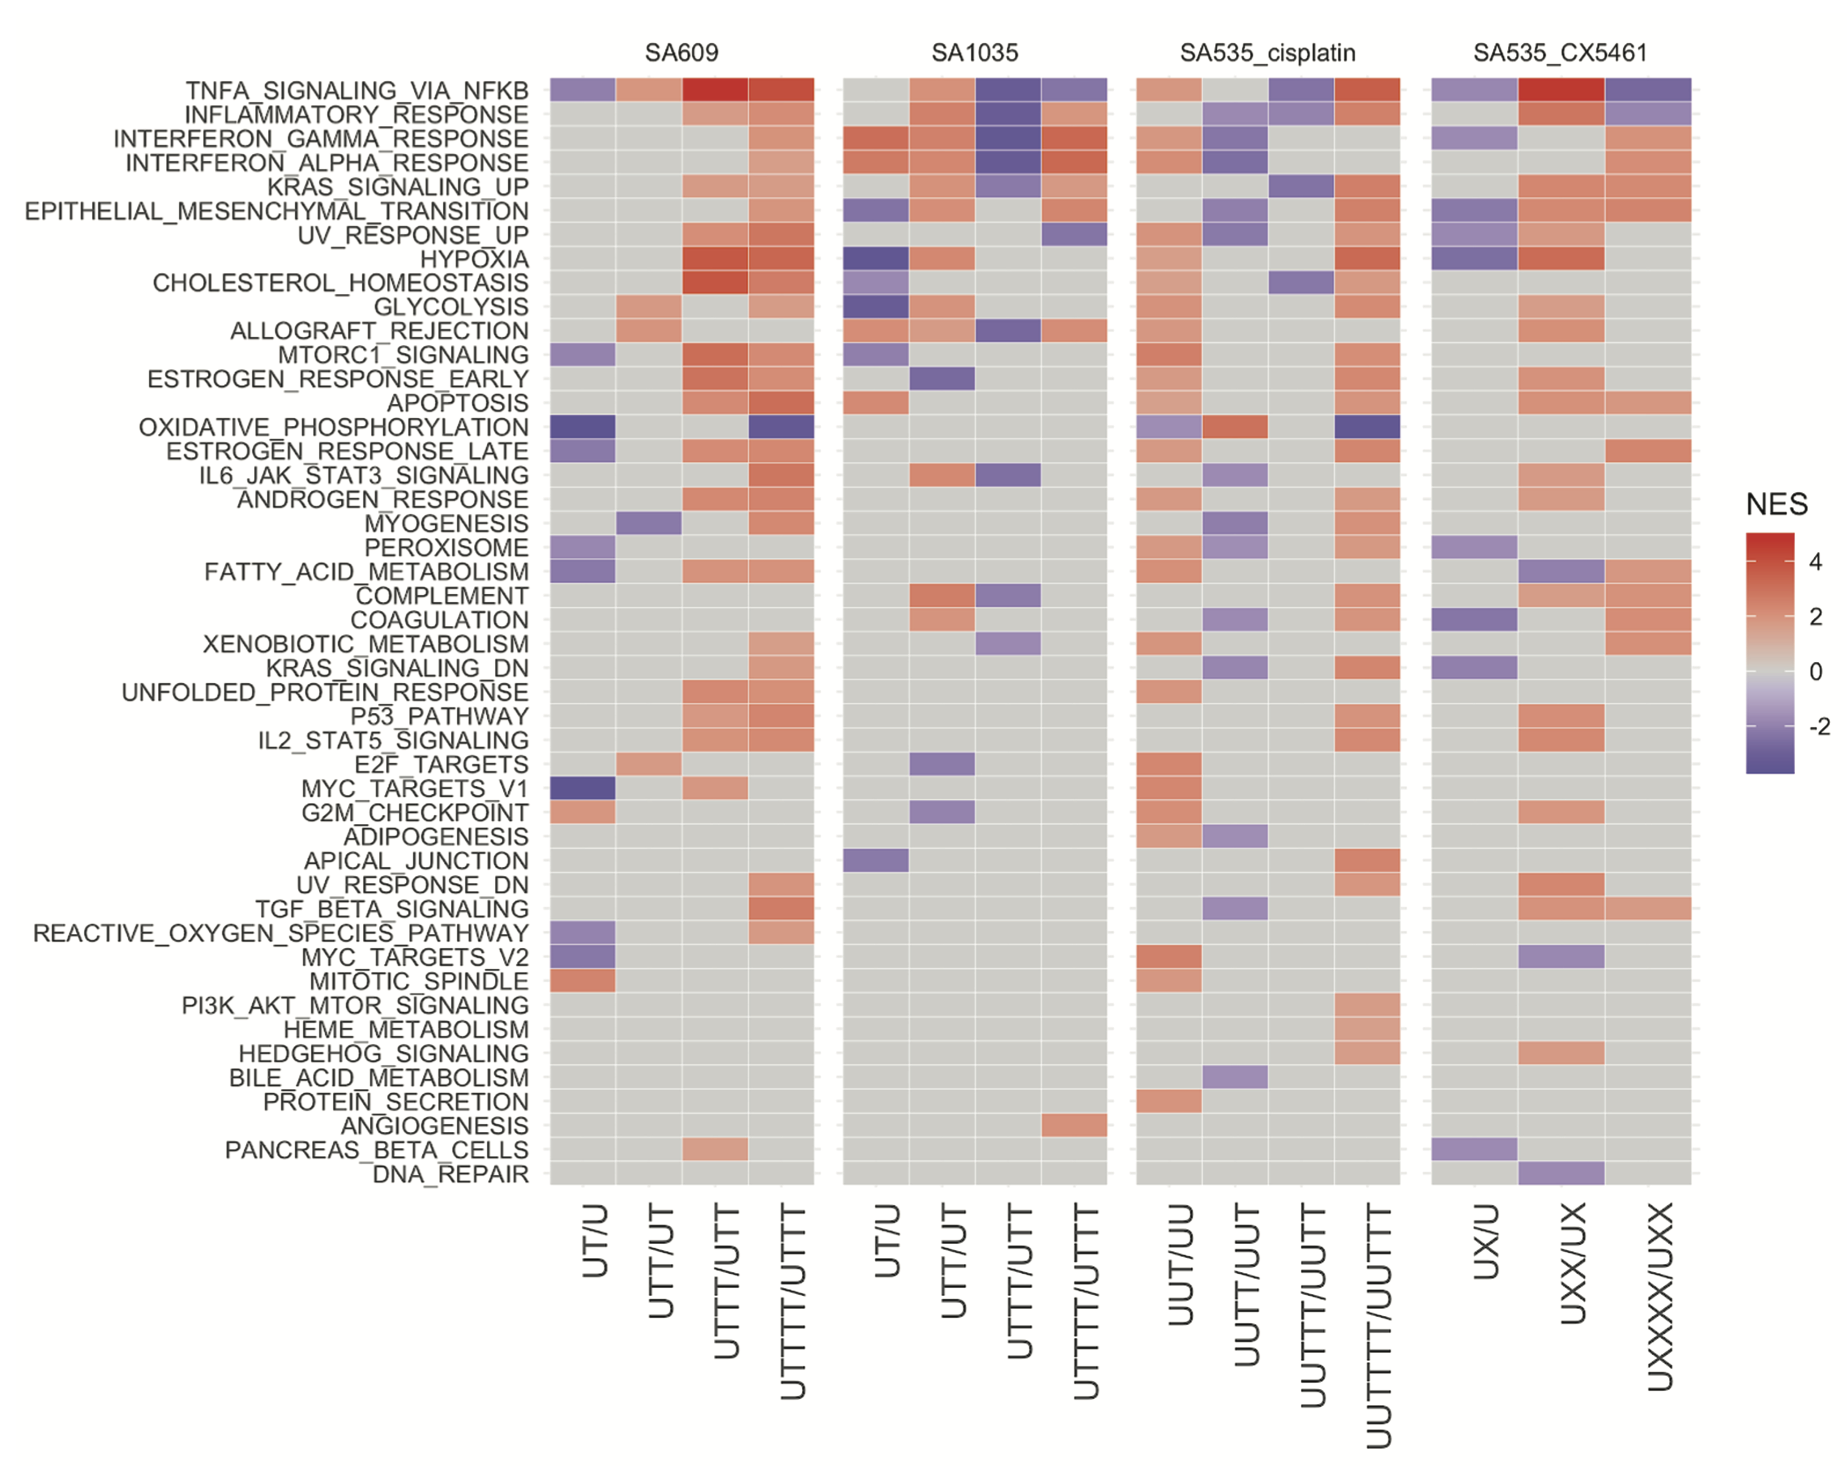
\includegraphics[width=\textwidth]{Figures/chap5/pathwaysevolution.png}
%\caption[Summary of number of genes \textit{in-cis} and \textit{in-trans}]
%	{\small
%	\textbf{Pathways comparison over time under chemotherapy in all PDX series}
%	Vertical left column enlist the pathways analysed. Horizontal axis at the bottom, represents the comparisons made between the time points and the treatment status. each single `T' indicates the number of cycles of the treatment from cisplatin. Each `X' indicates number of cycles of CX-5461 treatment. Colour intensity identifies normalized enrichment score (NES). Horizontal axis on top denotes the IDs of TNBC PDX. A normalized enrichment score (NES) was calculated from a ranked gene set enrichment analysis (GSEA) \cite{shi2007gene} performed on each subset of differentially expressed genes using the hallmark gene set collection from MSigDB \cite{liberzon2015molecular}.  Significantly enriched pathways (adjusted p-value $<$ 0.01).
%}
 %   \label{fig:pathwaysevolution}
%    \end{figure}
%-------------------------------------------------------------------
\begin{figure}
\centering
  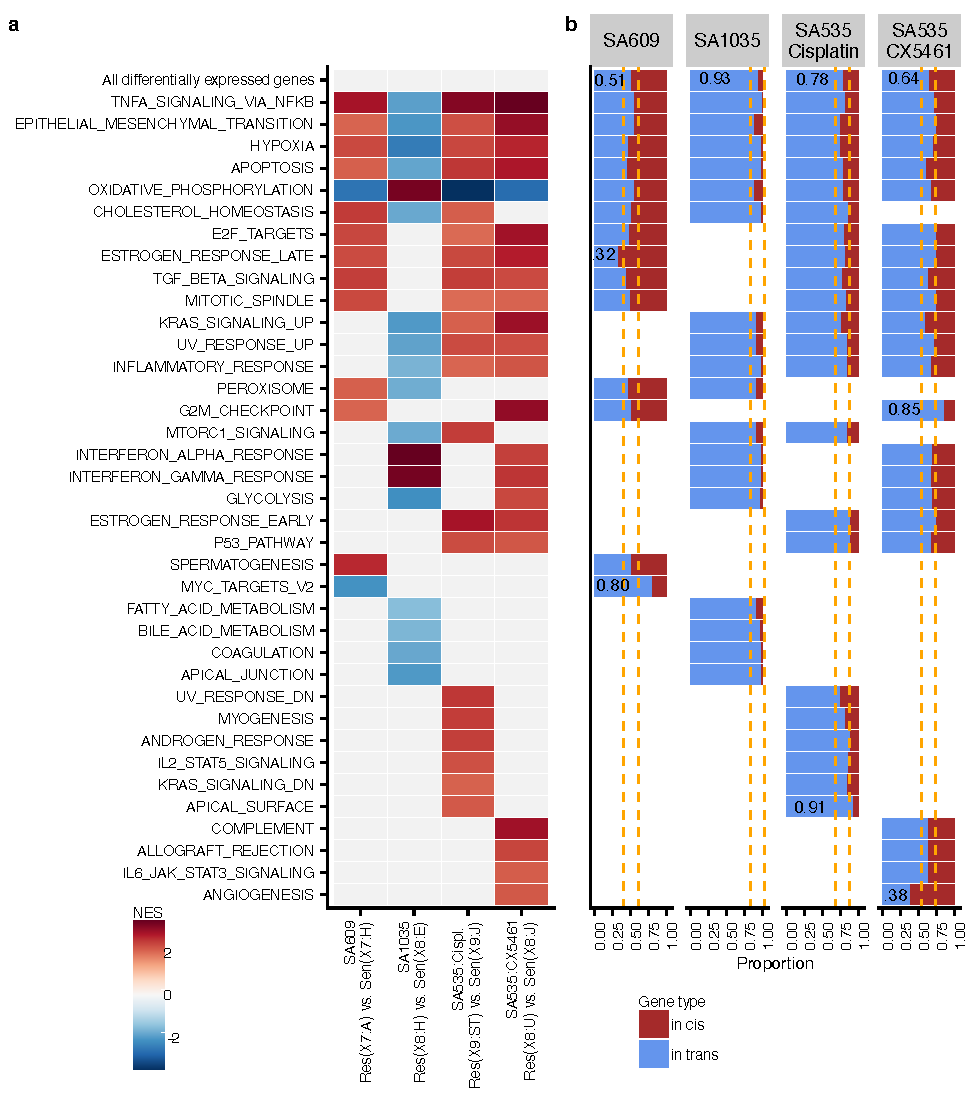
\includegraphics[width=\textwidth]{Figures/chap5/fig13_common_pathways.pdf}
\caption[Gene pathway enrichment analysis of PDX timeseries]
	{\small
	\textbf{Significantly enriched pathways} ($p < 0.05$, vertical axis) from a ranked gene set enrichment analysis (GSEA) \cite{shi2007gene}, using the hallmark gene set collection from MSigDB \cite{liberzon2015molecular}. \textbf{(a)} Horizontal axis denotes the IDs of TNBC PDX and clones. Colour intensity identifies normalized enrichment score (NES) obtained by using all the differentially expressed genes at the specified time points and clones at FDR $< 0.01$. \textbf{(b)} \textit{In cis} (red) and \textit{in trans} (blue) gene proportions for each case depicted in panel \textbf{a}. Vertical dashed lines show the expected proportions (defined as the proportions of all differentially expressed genes, top row) plus or minus 10\%. The cases that are outside of the expected range are marked by the \textit{in trans} proportion numbers.
	}
	\label{fig:pathwaysnetwork}
\end{figure}

%-------------------------------------------------------
%-------------------------------------------------------------------
\begin{figure}
\centering
  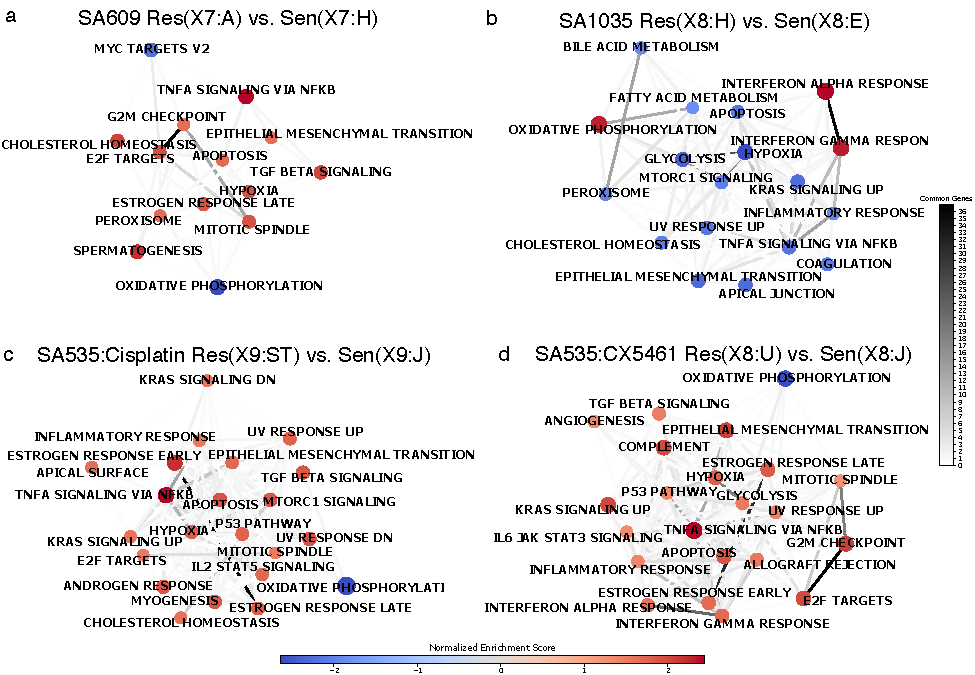
\includegraphics[width=\textwidth]{Figures/chap5/fig14_networks.pdf}
\caption[Gene pathway relationships of PDX timeseries]
	{\small
	\textbf{Networks showing the relationship between the enriched pathways in \textbf{\autoref{fig:pathwaysnetwork}}}. The color intensity denotes the normalized enrichment score (NES). The grey to black lines indicate the number of genes shared between pathways. \textbf{(a)} TNBC-SA609. \textbf{(b)} TNBC-SA1035.  \textbf{(c)} TNBC-SA535:Cisplatin. \textbf{(d)} TNBC-SA535:CX5461.
	}
	\label{fig:networks}
\end{figure}

%-------------------------------------------------------


%\subsection{Integrated transcriptome and pathway analyses revealed potential genes and key activated pathways in breast cancer}
%Next, we performed gene set enrichment analysis (GSEA) to search for sets of genes that are significantly over-represented in a given list of genes, compared to a background set of genes and their respective pathways and network connections. 
%First, We generated a heatmap of pathway evolution from one treated time point to another in all timeseries TNBC PDX \textbf{\autoref{fig:pathwaysevolution}}. Most of the listed pathways were enriched at the later timepoints, where tumors started developing chemoresistance. 

%\subsubsection{Profiling of signaling pathways reveals a distinct demarcation between SA1035 and rest of 3 TNBC PDX}
\subsubsection{Integrated transcriptome and pathway analyses revealed potential genes and key activated pathways in breast cancer}
To assess the common pathways and their network connections, 
we profiled pathway enrichment scores between the resistant and sensitive clones of all TNBC PDX at the late time points:  X7 for TNBC-SA609, X8 for TNBC-SA1035, X9 for TNBC-SA535-cisplatin and X8 for TNBC-SA535-CX-5461 (\textbf{\autoref{fig:pathwaysnetwork}}). 
Pathway specific differentially expressed genes were included in network enrichment analysis and the nodes were coloured by the normalized enrichment score (NES). Interestingly, TNBC-SA1035 PDX demonstrated only three upregulated pathways in resistant versus sensitive clone, including \textbf{Oxidative phosphorylation (OXPHOS)}, \textbf{Interferon alpha response} \cite{provance2019deciphering} and \textbf{Interferon gamma response} \cite{mojic2018dark} (\textbf{\autoref{fig:pathwaysnetwork} a}, second column). \textbf{\ac{OXPHOS}} is known to be upregulated in cisplatin related drug resistance mechanism \cite{lee2017myc}. The latter two pathways are not well studied in relation to tumor progression or drug resistance but there is some speculative research related to these interferons and cancer related immune mechanisms. In contrast to other TNBC PDX, TNBC-SA1035 resistant clone also evinced downregulated pathways of \textbf{Hypoxia}, \textbf{TNFA signaling via NF-$\kappa$B}, \textbf{\ac{EMT}}, \textbf{MTORC1 signaling}, \textbf{KRAS signaling} and \textbf{Apoptosis} ({\textbf{\autoref{fig:pathwaysnetwork} c}}). The genes involved in these pathways are shown in \textbf{\autoref{fig:genenetworkanalysis} b}.

In addition to TNBC-SA1035, only TNBC-SA535 timeseries that was treated with CX-5461 showed interferons pathways upregulation. However, the rest of 3 TNBC PDX, TNBC-SA609, TNBC-SA535-cisplatin treated and TNBC-SA535-CX-5461 treated, showed commonly upregulated certain pathways, including, \textbf{TNFA signaling via NF-$\kappa$B} \cite{lagunas2008nuclear,ito2015down, ryan2019targeting}, \textbf{Hypoxia} \cite{lee2012hypoxia, mcevoy2015identifying, deben2018hypoxia,li2019erk}, \textbf{Apoptosis} \cite{panaretakis2012cisplatin}, \textbf{TGF Beta signaling} \cite{zhang2019tgfbeta1} and \textbf{Estrogen response} \cite{zhu2018er}. \textbf{E2F targets} \cite{zheng2020upregulation} and \textbf{G2M checkpoint} \cite{visconti2016cell} were common between TNBC-SA609 and TNBC-SA535-CX-5461 treated (\textbf{\autoref{fig:pathwaysnetwork} a}, first, third and fourth columns). 



%\begin{figure}
%\centering
%  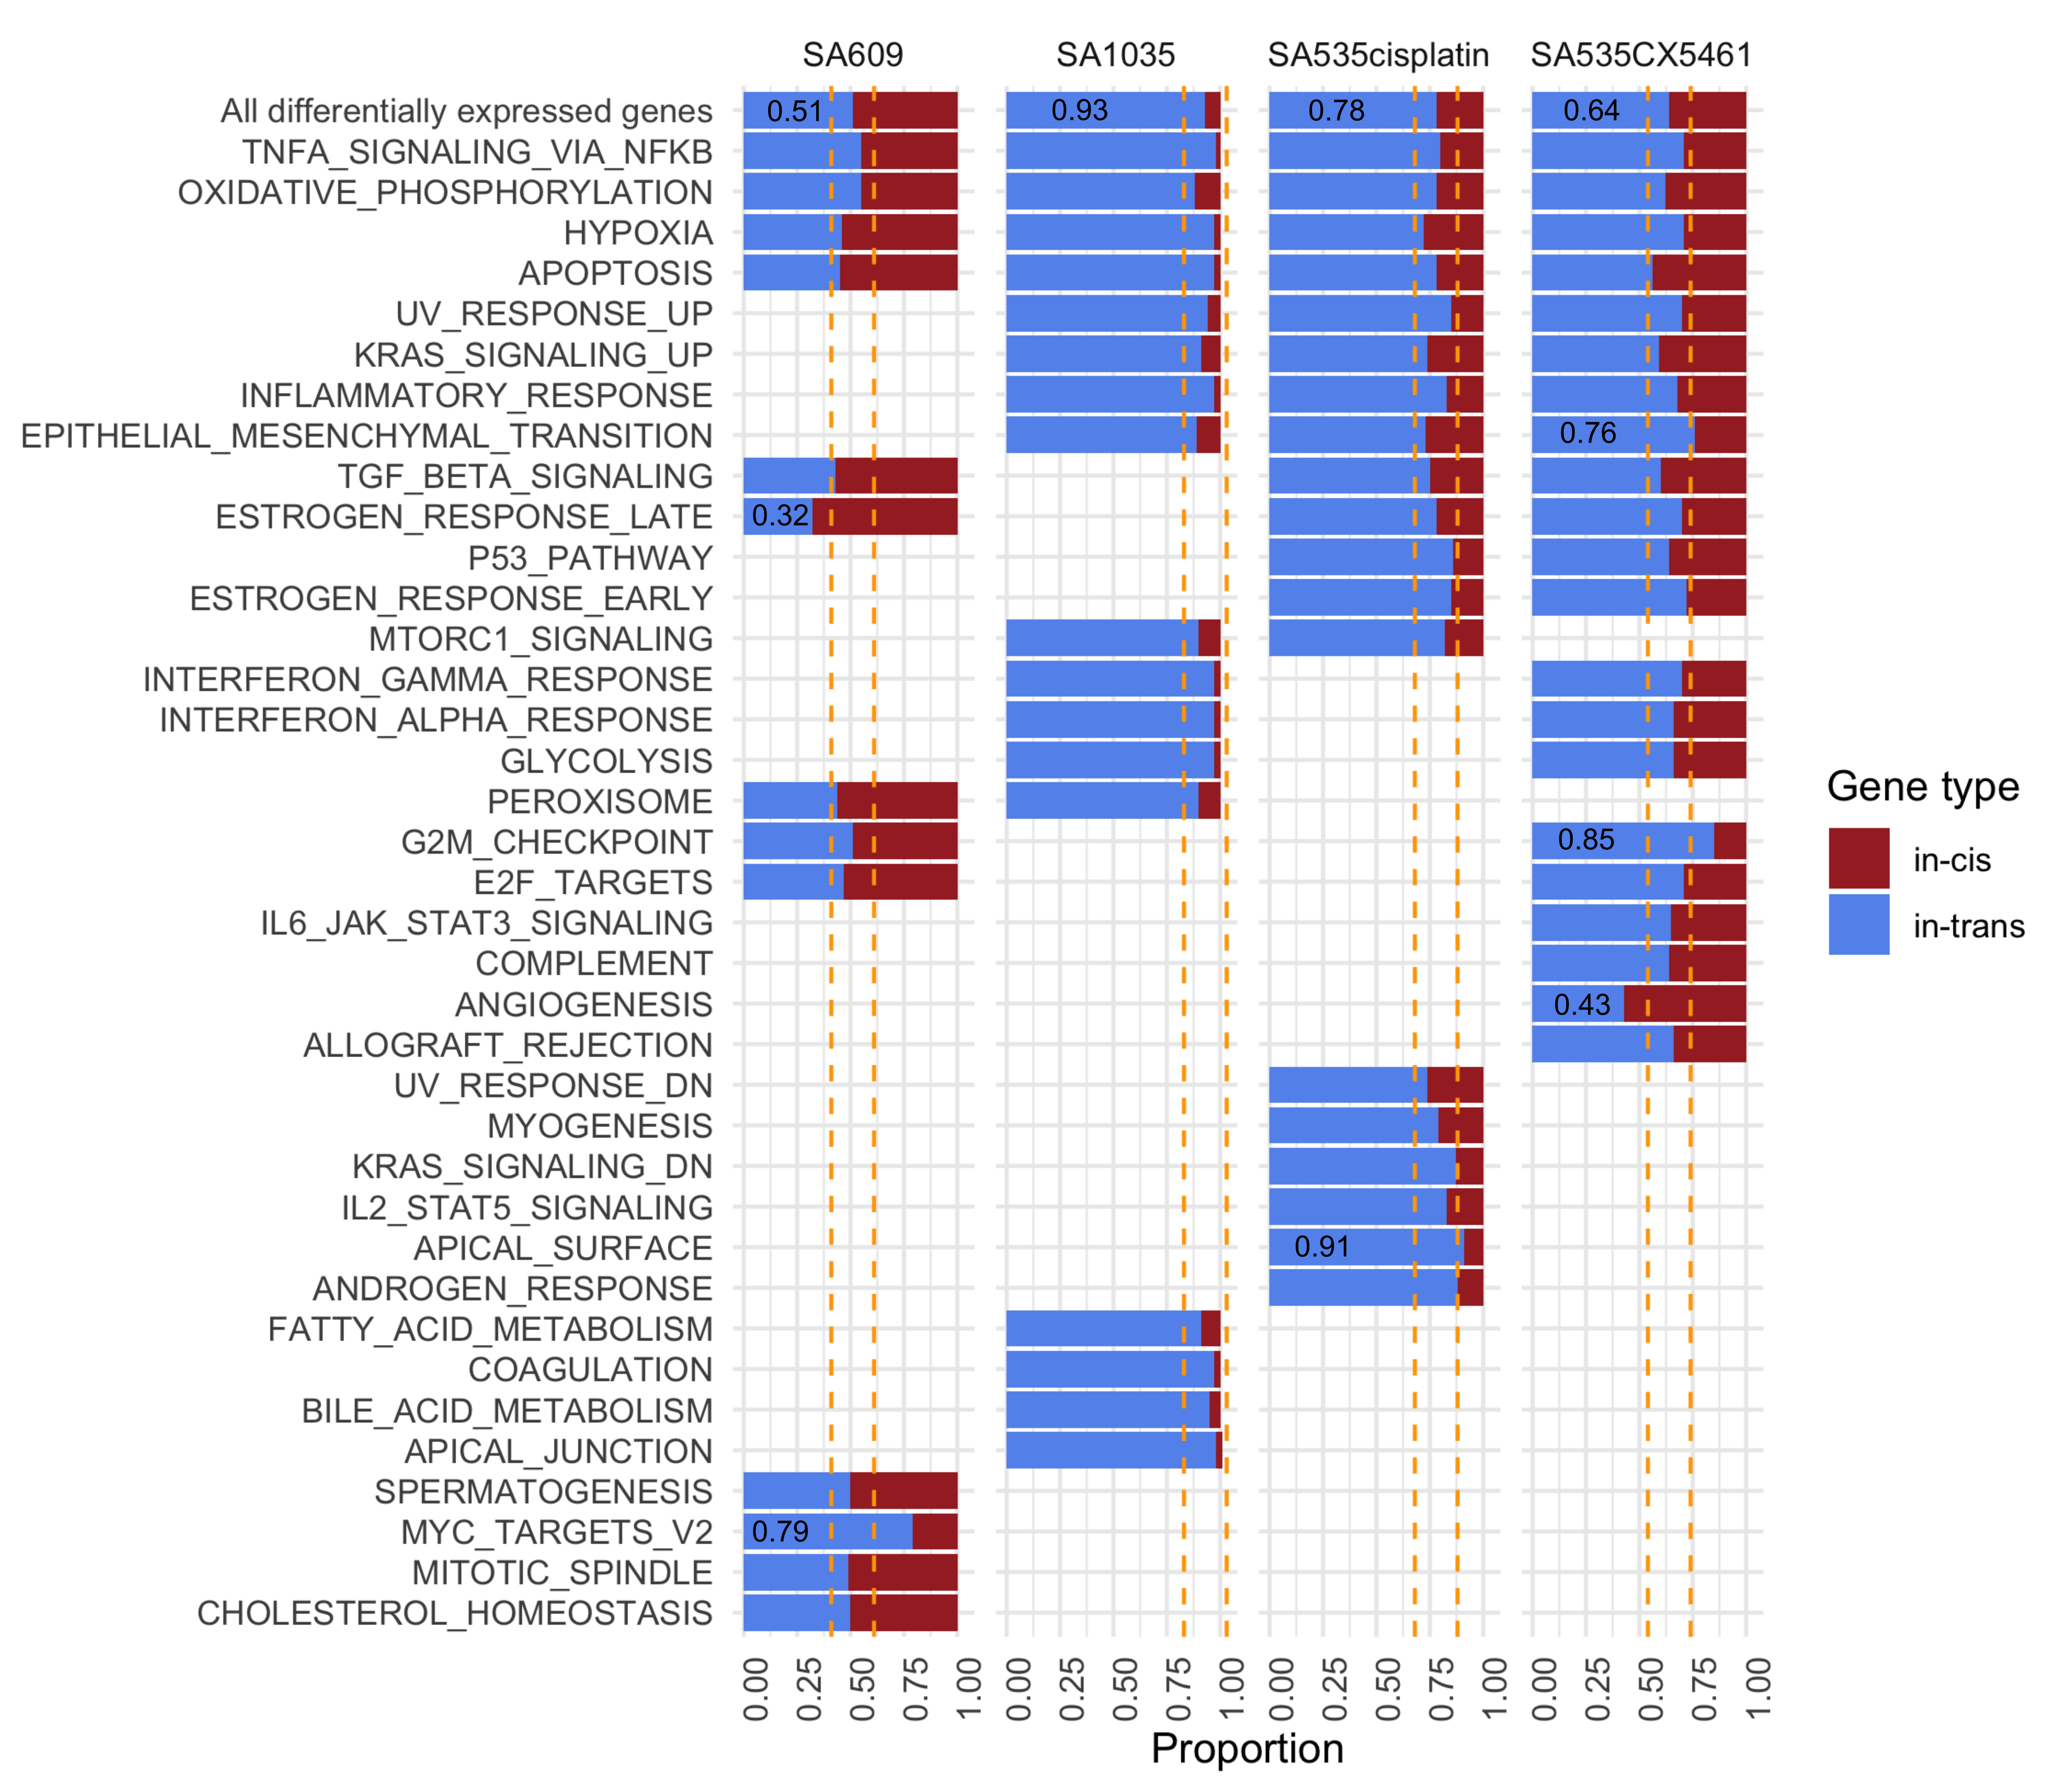
\includegraphics[width=\textwidth]{Figures/chap5/cistransproportionsinpathways.png}
%\caption[Proportions of \textit{in cis} and \textit{in trans} regulated genes in pathways]
%	{\small
%	\textbf{Proportions of \textit{in cis} and \textit{in trans} regulated genes in pathways.}
%	 	Vertical axis on the left enlists the gene set enrichment analysis (GSEA) pathways in the same order as in \textbf{\autoref{fig:pathwaysnetwork}}, with the addition of a new row on top for all the differentially expressed genes. For each set of genes and each series, the proportion of \textit{in cis} (red) and \textit{in trans} (blue) genes was calculated. The \textit{in trans} proportions for all genes (top row) are given. Vertical dashed lines show the expected proportions, defined as the proportions in all genes (top row), plus or minus 10\%. The observed proportions outside of this range are identified. 
%	}
%	\label{fig:cistransproportionsinpathways}
%\end{figure}


%------------------------------------------------------------------

% text about the in-cis in-trans proportions figure 
The proportions of \textit{in cis} and \textit{in trans} genes in the gene set enrichment pathways are within 10\% of the proportion in the entire population of genes for most pathways, with only a few exceptions (\textbf{\autoref{fig:pathwaysnetwork} b}). In TNBC-SA609 (expected \textit{in trans} proportion 0.51), \textbf{Estrogen response late} pathway has a lower percentage of \textit{in trans} genes (0.32), while \textbf{MYC targets V2} has a higher percentage of \textit{in trans} genes (0.79). In TNBC-SA1035 all pathway proportions are within the expected range (0.93 \textit{in trans} proportion). In TNBC-SA535-cisplatin (expected \textit{in trans} proportion 0.78), only \textbf{Apical surface} pathway has a higher \textit{in trans} proportion of 0.91. Finally, in TNBC-SA535-CX-5461 (expected \textit{in trans} proportion 0.78), \textbf{EMT} and \textbf{G2M checkpoint} pathways have a higher \textit{in trans} proportion (0.76 and 0.85, respectively), and \textbf{Angiogenesis} has a lower \textbf{in trans} proportion of 0.43.

To portray pathway specificity in resistant versus sensitive clones, we explored \textbf{SA609 TNBC PDX}, which was  comprised of \textbf{TGF Beta signaling, Hypoxia, TNFA signaling via NF-$\kappa$B, Cholesterol homeostasis, Peroxisome} and \textbf{Apoptosis} (\textbf{\autoref{fig:pathwaysnetwork} b}). In addition to these, \textbf{G2M checkpoint} and \textbf{E2F targets} were found to be upregulated with $>$40 common genes between these two pathways. \textbf{Mitotic spindle} pathway upregulation was also associated with sharing of $>$10 genes with \textbf{E2F} and \textbf{G2M check point} pathways \textbf{\autoref{fig:genenetworkanalysis} a}.

%--------------------------------------------------------------------

\subsubsection{TNBC-SA535 PDX reveals specificity of drugs in pathway network inference} 
As \textbf{TNBC-SA535 PDX} was treated with two different drugs, cisplatin and CX-5461 in parallel (\textbf{\autoref{fig:SA535CX5461} a}), we explored how many pathways are comparable in these two series and which ones are distinct or unique to each specific drug. 
We found that \textbf{11 pathways} were upregulated and only one, which was \textbf{\ac{OXPHOS}}, was down regulated in both series, suggesting their specificity to the tumor itself. The list of these pathways encompass \textbf{TNFA signaling via NF-$\kappa$B, Hypoxia, Apoptosis, UV response up, KRAS signaling up, Inflammatory response, Epithelial mesenchymal transition, TGF Beta signaling, Estrogen response} and \textbf{p53} pathways ({\textbf{\autoref{fig:pathwaysnetwork} a} third \& fourth column upper half and \textbf{\autoref{fig:pathwaysnetwork} d, e}). However, there were certain pathways that were definitive to one of the two drugs. The cisplatin treated resistant clone was found to have exclusively upregulated pathways including \textbf{MTORC1 signaling \cite{peng2010role}, KRAS signaling down} \cite{tao2014oncogenic}, \textbf{IL-2\_STAT5 signaling \cite{wu2020activation, gutierrez2020role}, Apical surface} (genes encoding proteins over-represented on the apical surface of epithelial cells, e.g., apical area important for cell polarity) \cite{halaoui2015rewiring, wodarz2007cell}, \textbf{UV response down} (including \textbf{UV\_response\_Via\_ERCC3\_TTD\_DN}
and \textbf{UV\_response\_Via\_ERCC3\_XPCS\_DN}) and \textbf{Androgen response} pathways \cite{rampurwala2016role, michmerhuizen2020we}.}

Within cisplatin treated activated pathways, \textbf{Hypoxia, TNFA signaling via NF-$\kappa$B, MTORC1, Estrogen response} and \textbf{Inflammatory response} related pathways share the most common genes among their network (\textbf{\autoref{fig:pathwaysnetwork} e}). The genes that are expressed are shown in  \textbf{\autoref{fig:genenetworkanalysis} c}. However, CX-5461 treated resistant clone came up particularly with \textbf{G2M checkpoint, E2F targets, IL-6\_JAK\_STAT3 signaling, Angiogenesis, Complement system} (genes encoding components of the complement system, which is part of the innate immune system), \textbf{Interferon alpha response, Interferon gamma response} and \textbf{Glycolysis} (\textbf{\autoref{fig:pathwaysnetwork} d}). Among these pathways, \textbf{G2M checkpoint} and \textbf{E2F targets} pathways share $>$30 genes, whereas, \textbf{\ac{EMT}, TNFA signaling via NF-$\kappa$B, Hypoxia} and \textbf{Glycolysis} share $>$ 15 genes. The gene network with related pathways are shown in  \textbf{\autoref{fig:genenetworkanalysis} d}. 

%-------------------------------------------------------
\begin{figure}
\centering
 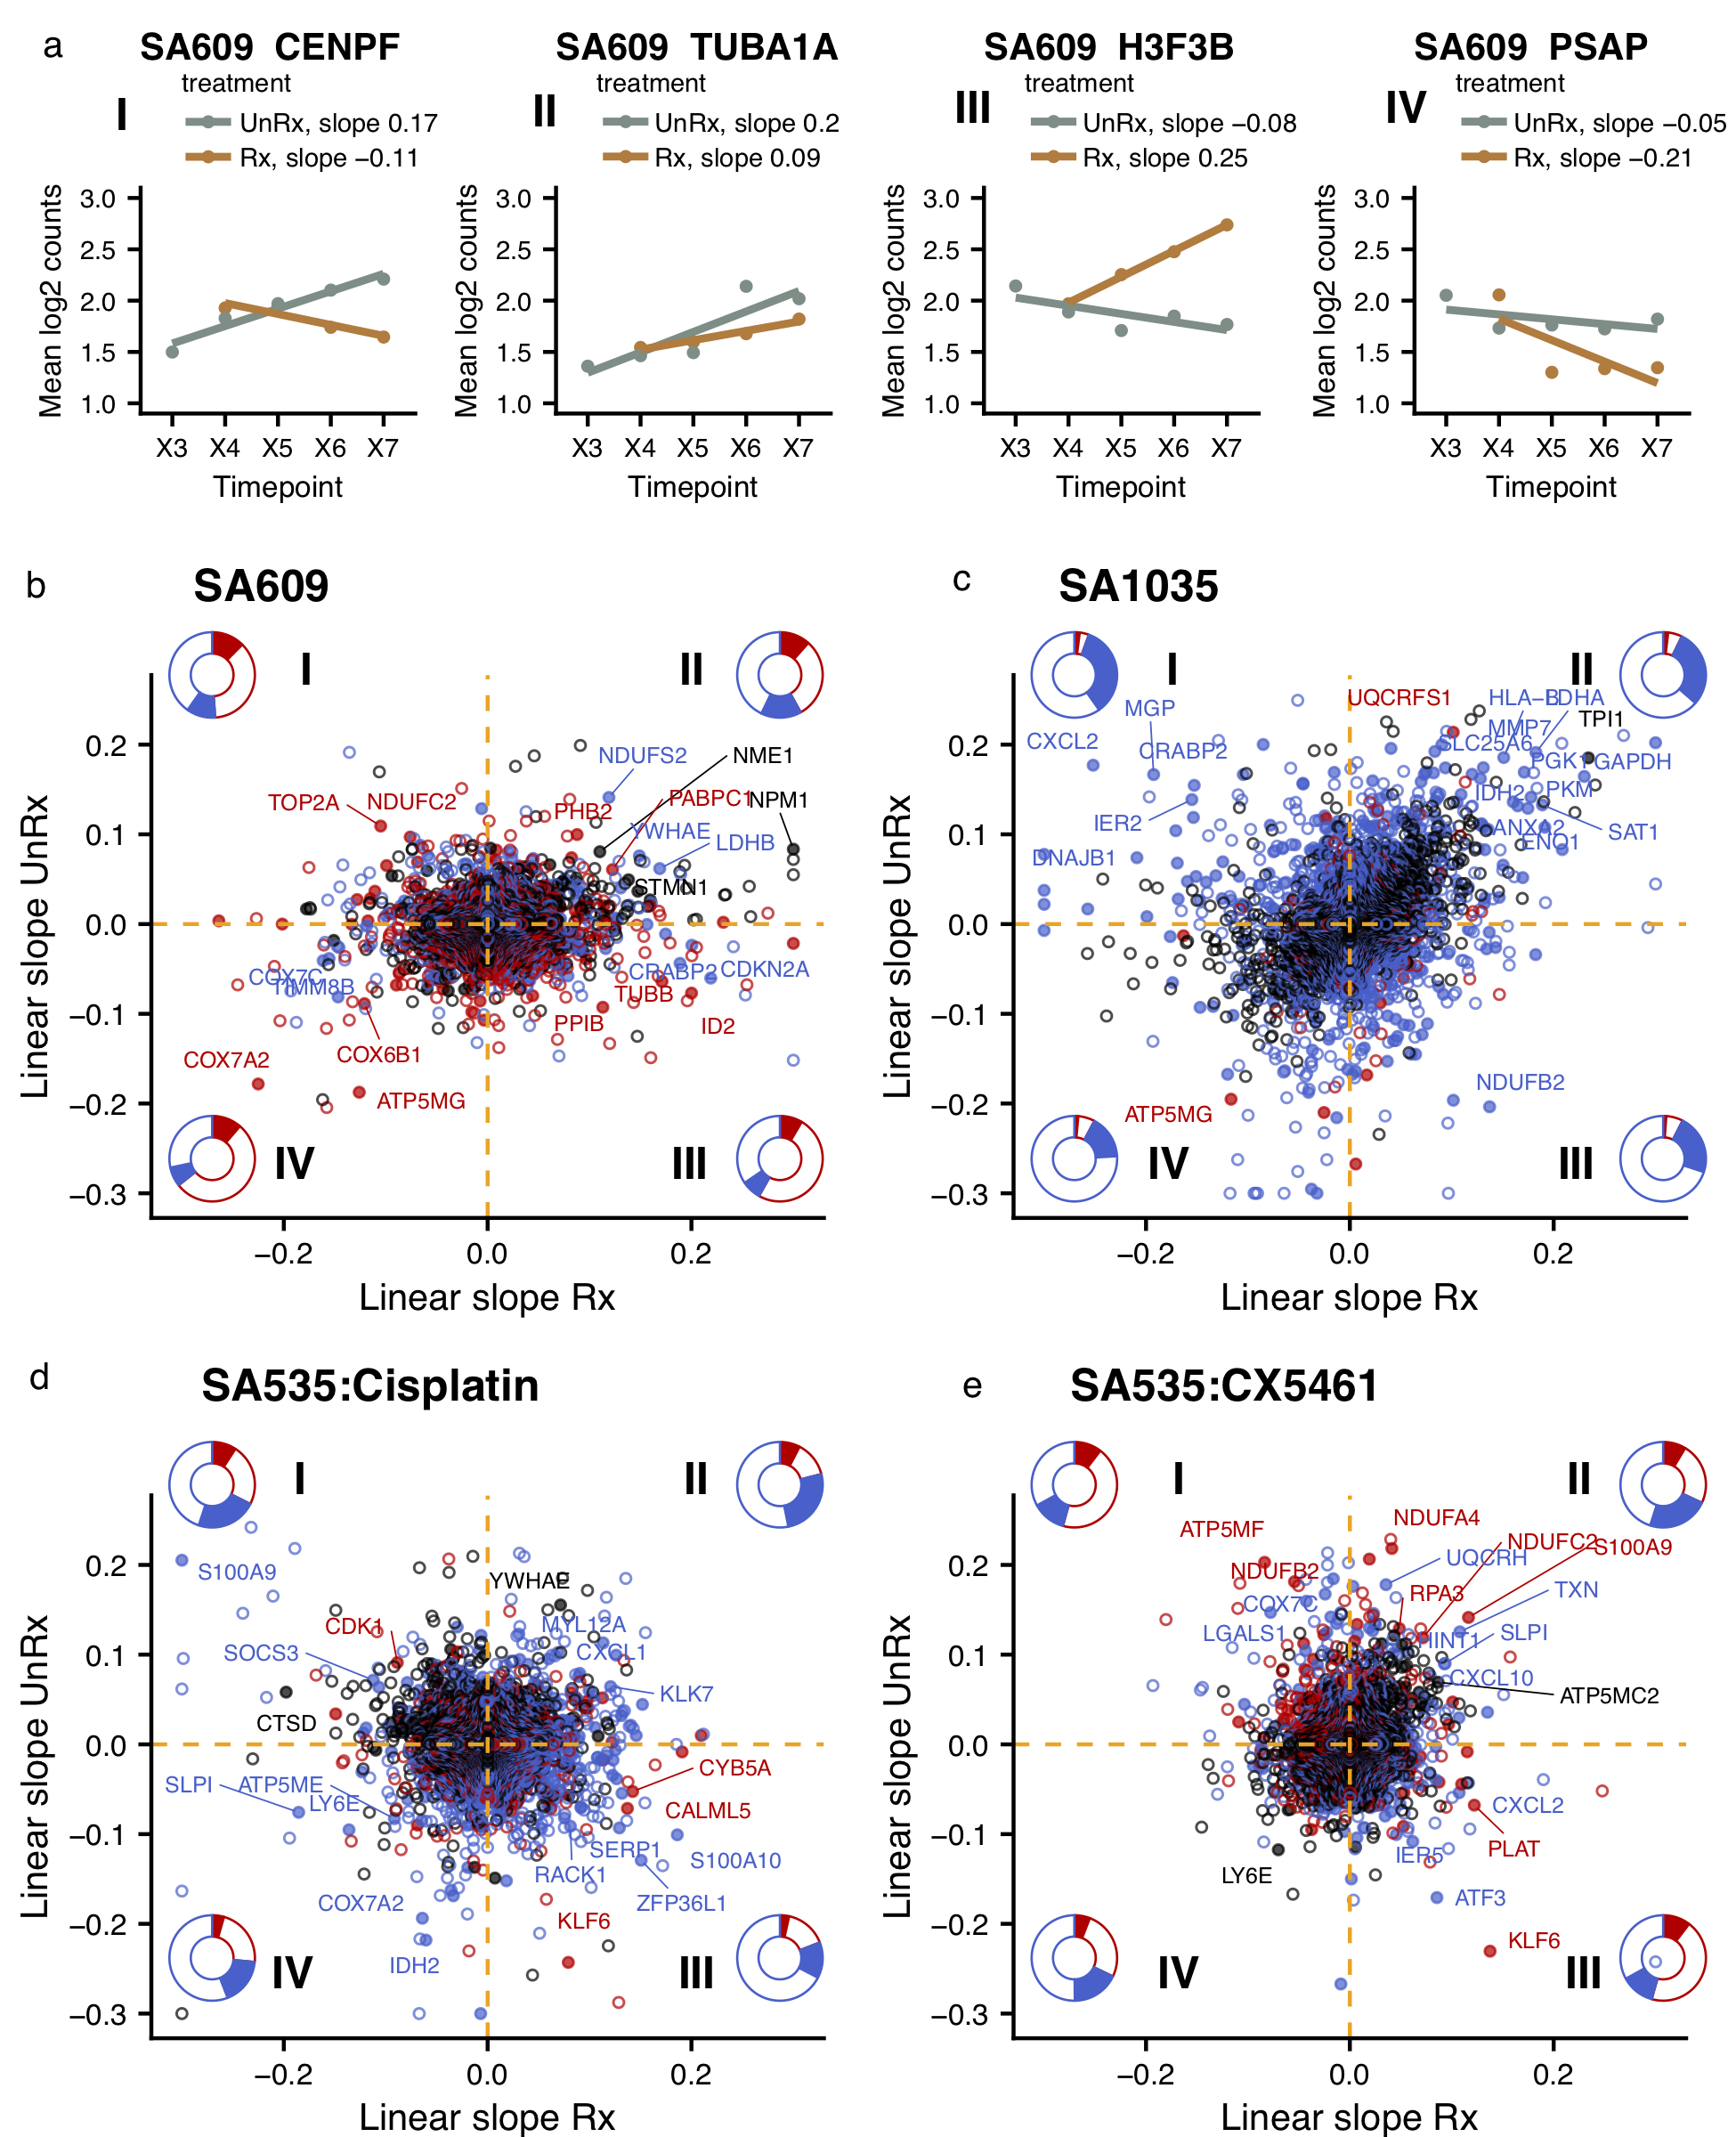
\includegraphics[width=\textwidth]{Figures/chap5/fig15_GeneschanginginRxclouds.png}
\caption[Gene expression changes over time with and without treatment in all 4 TNBC PDX timeseries]
	{\small
	 \textbf{Gene expression changes over time with and without treatment}.
\textbf{(a)} Examples of linear model fitting to mean SCTransform log2 normalized gene expression levels at the available treated and untreated time points. \textbf{(b)-(e)} Scatter plots of linear slopes showing the gene expression change across treatment cycles (x-axis) versus untreated cycles (y-axis). Each of the four quadrants are numbered as I (genes increasing without treatement and decreasing with treatment), II (increasing both in untreated as well as with treatment), III (increasing expression only with treatment and decreasing without drug) and  IV (decreasing with passaging over time in both untreated and treated tumors).  \textbf{(b)} TNBC-SA609. \textbf{(c)} TNBC-SA1035, Rx and UnRx X5 samples were eliminated from the slope calculation due to lower data quality. \textbf{(d)} TNBC-SA535:Cisplatin. \textbf{(e)} TNBC-SA535:CX5461.}

	\label{fig:GeneschanginginRxclouds}
\end{figure}

%-------------------------------------------------------------------

\subsection{Gene expression changes over time}

\subsubsection{Gene specific expression trajectories exemplified systematic response to sustained treatment}
%To understand the stability of gene expression throughout the treatment, we performed gene regression analysis on the top 500 resistant clone related genes and plotted their trend along various timepoints. All four treated PDX series manifested 2-3 distinct clusters with monotonically increasing, monotonically decreasing, remaining constant or irregular patterns \textbf{\autoref{fig:GeneschanginginRxclouds}}. Some of the gene clusters were found to be increasing or decreasing along the time series of the PDX models and require detailed investigation at individual gene level to get enough evidence.

To understand the gene expression dynamics over several treatment cycles in comparison with gene expression in consecutive untreated time points, we performed linear model fitting over the mean SCTransform log2 normalized gene expression levels at 3-5 time points (\textbf{\autoref{fig:GeneschanginginRxclouds}}). The slope of the linear fitting signifies the overall magnitude of change from one time point to the next. Since the y axis is on a log2 scale, a slope of 1 means that, on average over time, the expression level doubles with every time point. Similarly, slopes 0.1 and 0.2 mean that, on average, the expression level increases by 7\% and 15\%, respectively, at every time point.

\textbf{\autoref{fig:GeneschanginginRxclouds} a} gives examples of linear fitting for four genes from TNBC-SA609 which changed in different directions. \textbf{\autoref{fig:GeneschanginginRxclouds} b-e} shows the untreated slope (y axis) versus the treated slope (x axis) for each gene in our four series, with the \textit{in cis} and \textit{in trans} genes shown in red and blue colours, respectively. The genes in quadrants II and IV changed in the same direction in both treated and untreated (up in II and down in IV), suggesting dynamics due to passage, and not due to treatment status. Conversely, the genes in quadrants I and III changed in the opposite direction in the treated samples versus the untreated samples, suggesting dynamics due to treatment status. While the vast majority of genes form a "cloud" around the origin, a number of genes display significant change. Between 13 and 202 genes are outside of the 5th and 95th percentiles in each quadrant.



%-------------------------------------------------------
\begin{figure}
\centering
 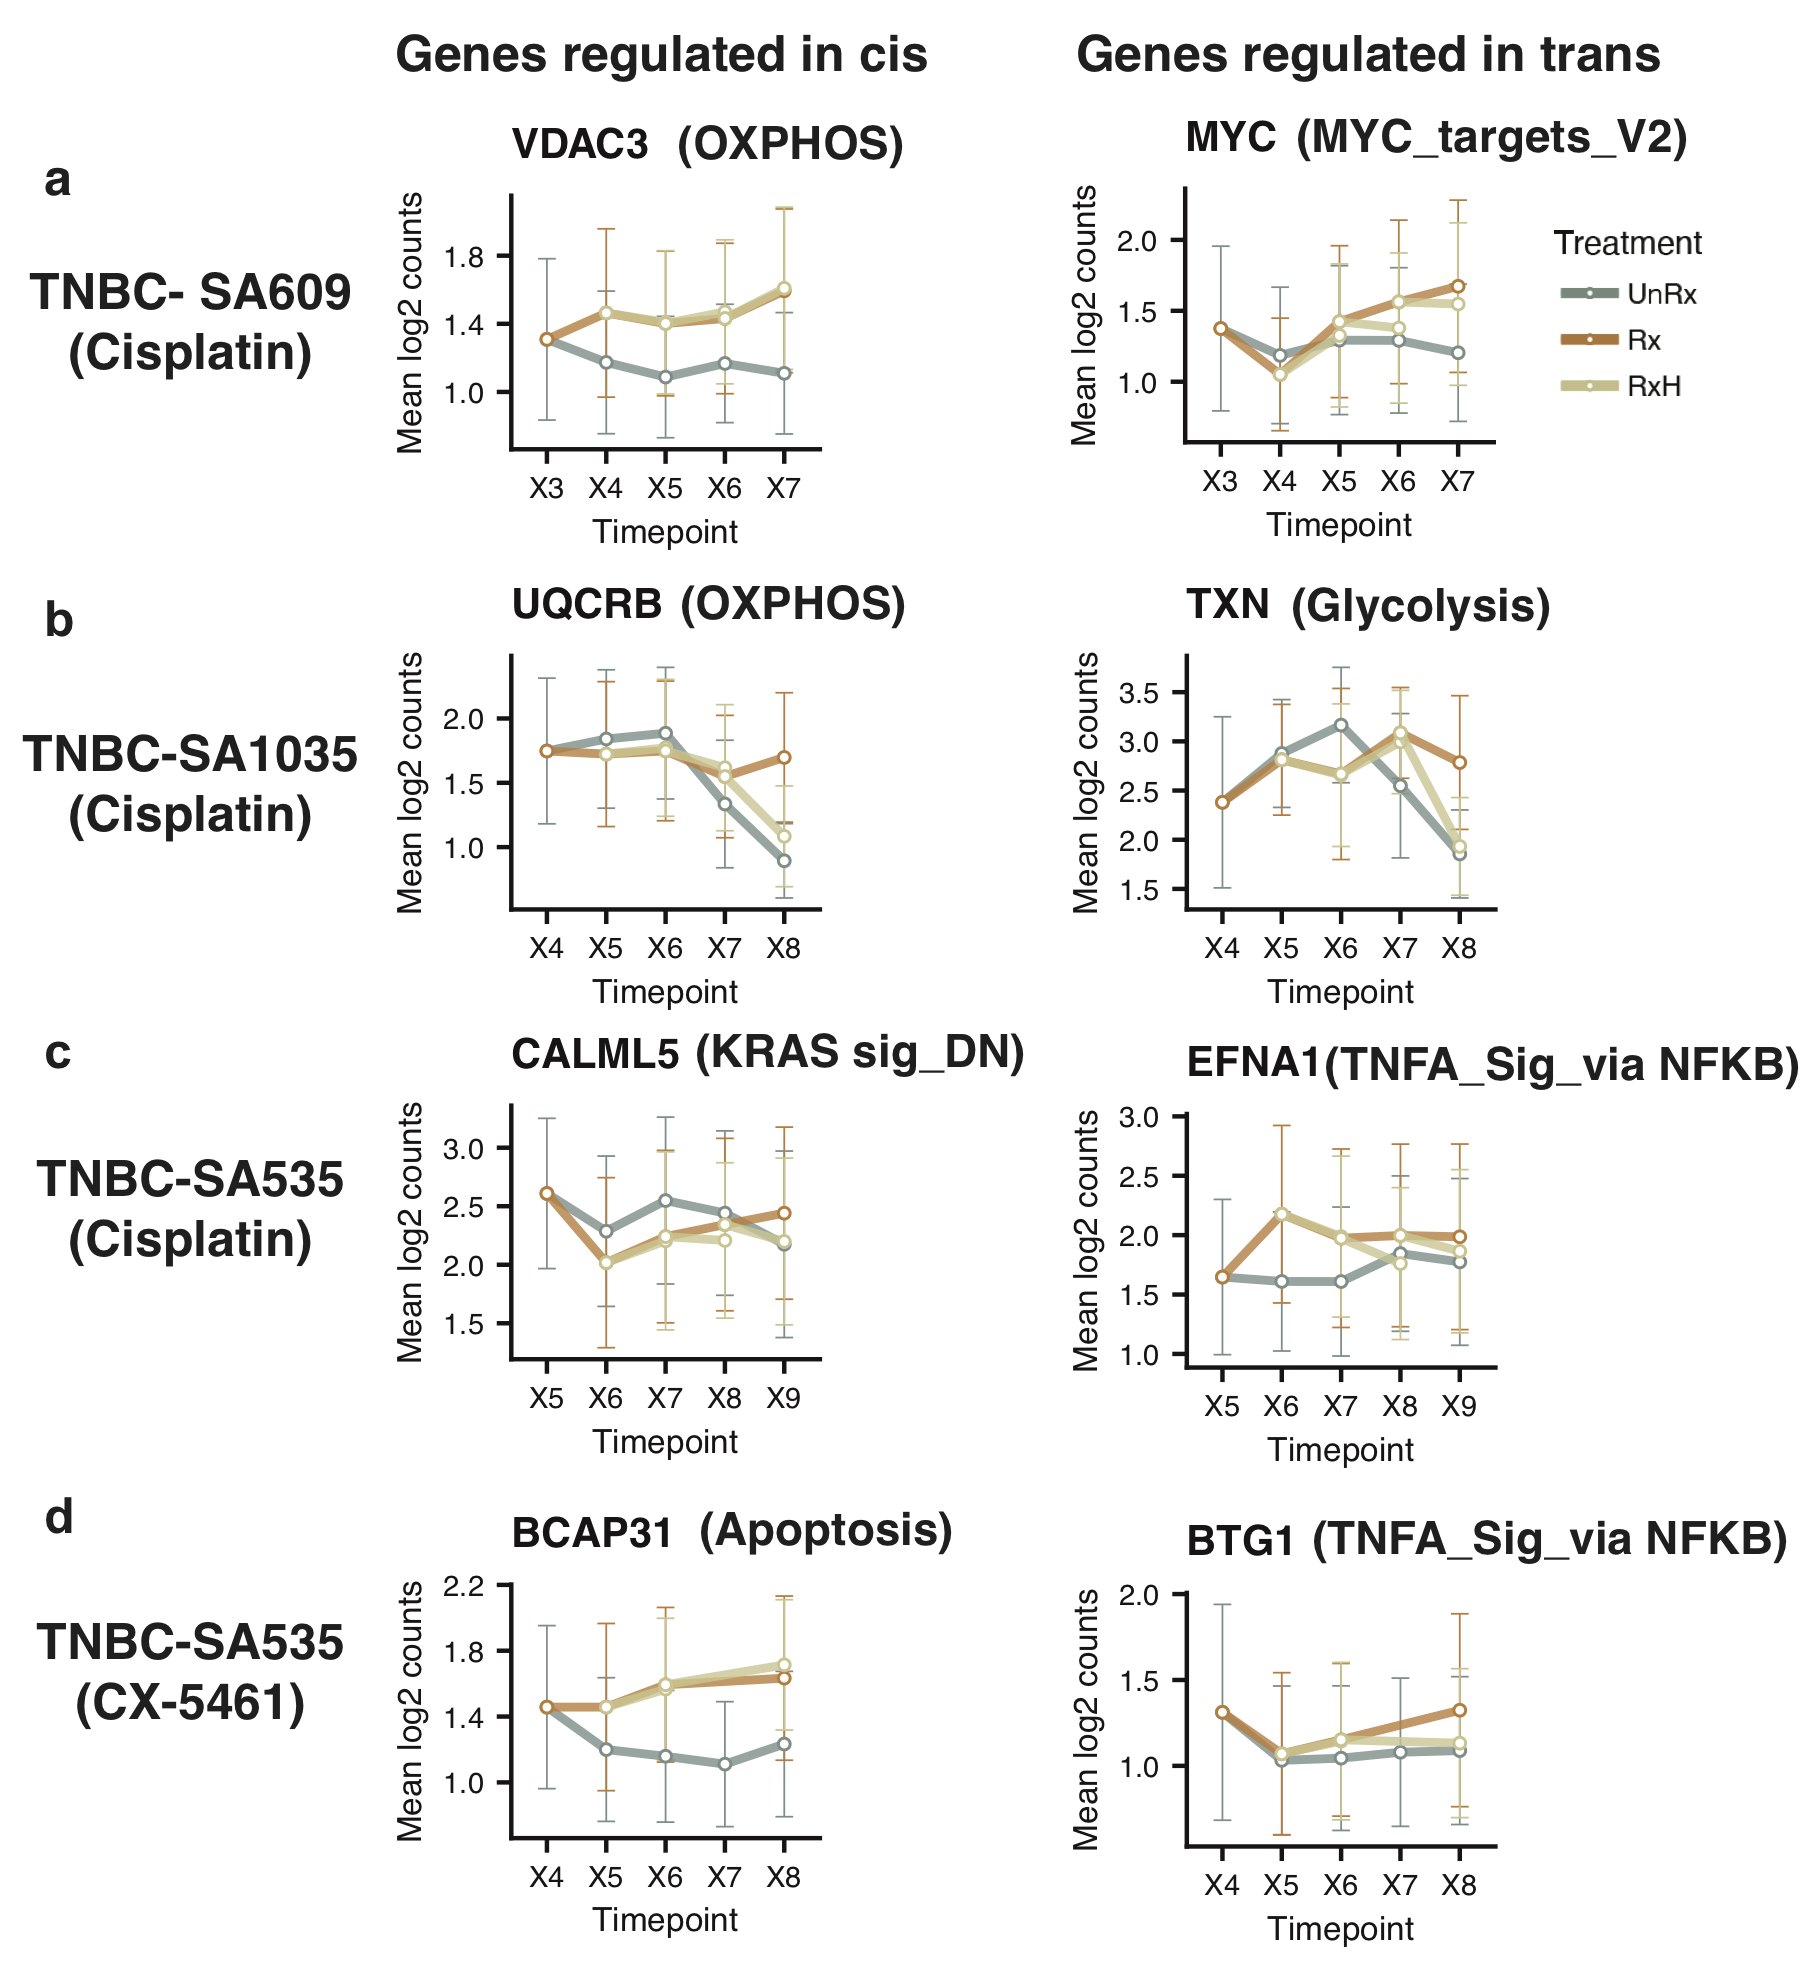
\includegraphics[width=\textwidth]{Figures/chap5/fig16_lineplotscistrans.png}
\caption[Example \textit{in cis} and \textit{in trans} genes]
	{\small
	 \textbf{Example \textit{in cis} and \textit{in trans} genes}.
	 }

	\label{fig:cistrans}
\end{figure}
%-------------------------------------------------------



%-------------------------------------------------------
\begin{figure}
\centering
 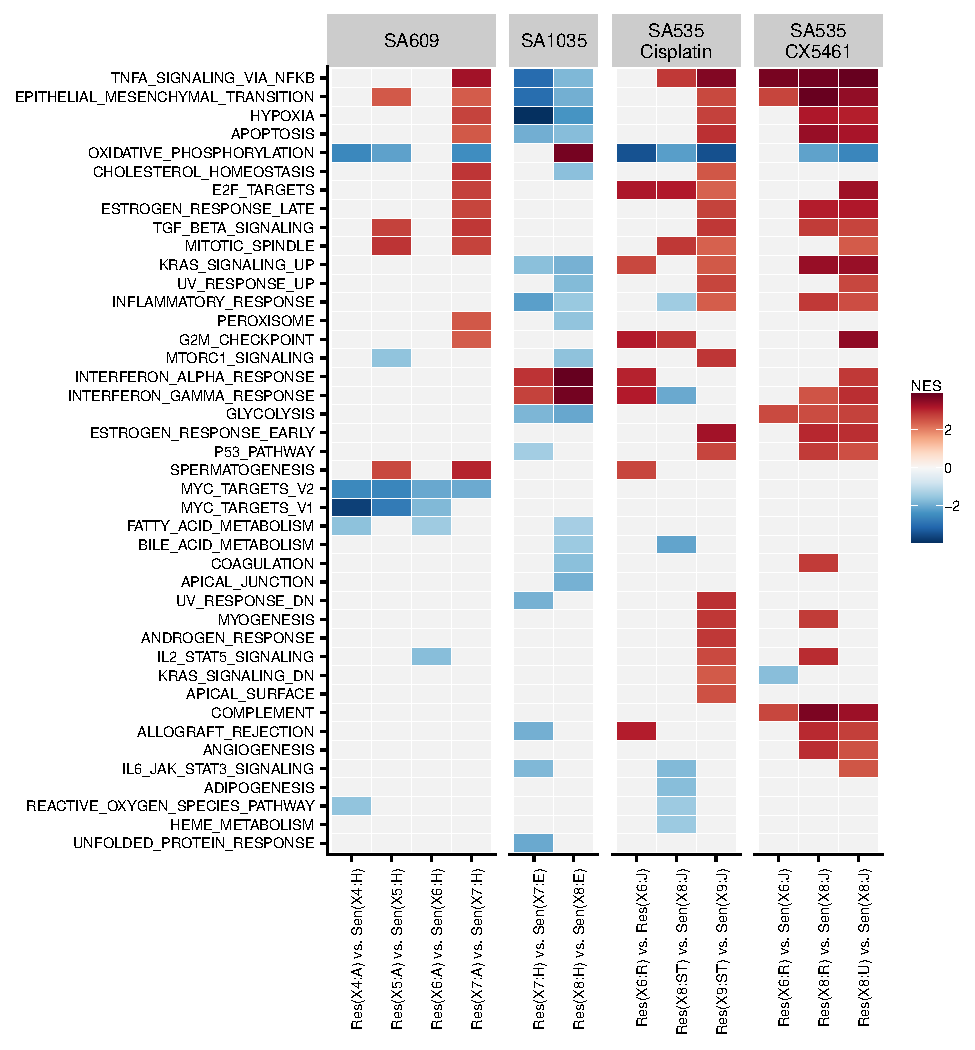
\includegraphics[width=\textwidth]{Figures/chap5/fig17_pathway_evolution.pdf}
\caption[Pathway evolution over passages]
	{\small
	 \textbf{Pathway evolution over passages}. GSEA pathway analysis similar to \textbf{\autoref{fig:pathwaysnetwork} a}, but now we also include earlier time points for each of the four TNBC PDX. For SA535, we also include the precursor resistant clone R at time point X6 for both cisplatin and CX5461, and at X8 for CX5461.
	 }

	\label{fig:pathwayevolution}
\end{figure}
%-------------------------------------------------------

%-------------------------------------------------------
\begin{figure}
\centering
 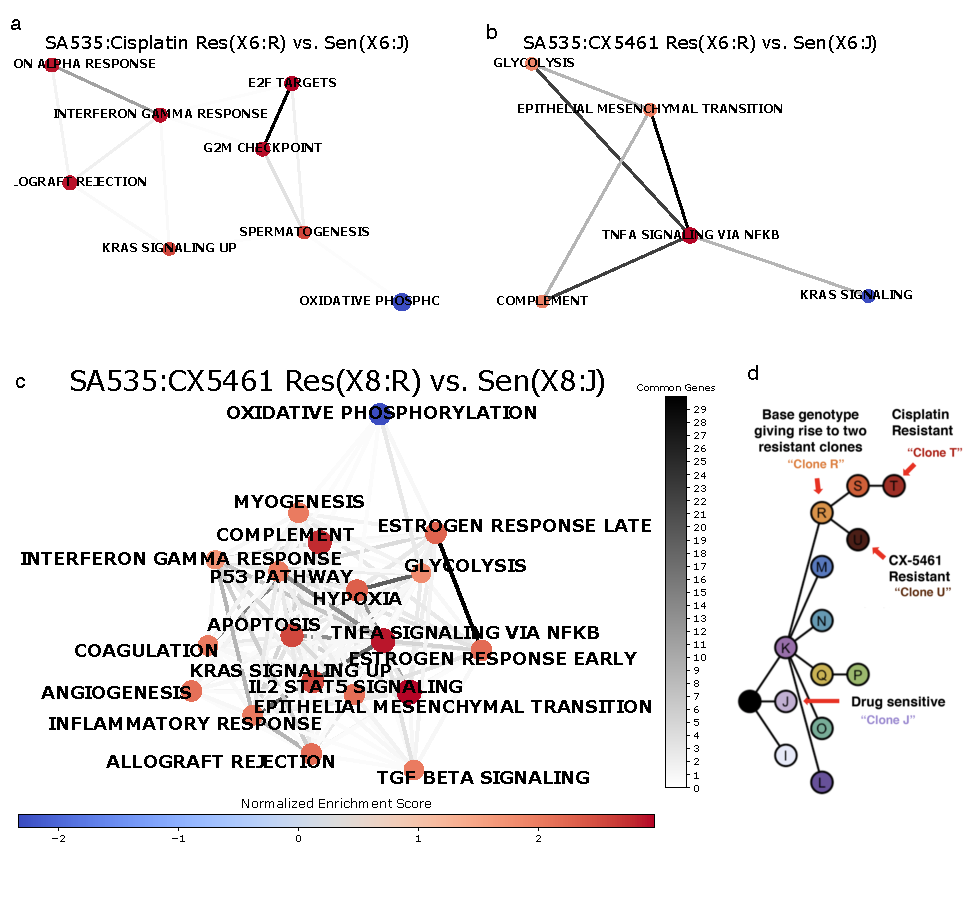
\includegraphics[width=\textwidth]{Figures/chap5/fig18_Rclone_pathways.pdf}
\caption[Pathway networks for the TNBC-SA535 precursor resistant clone.]
	{\small
	 \textbf{Pathway networks for the TNBC-SA535 precursor resistant clone R.} \textbf{(a)} Pathway network for SA535:Cisplatin comparing resistant clone R versus sensitive clone J at X6. \textbf{(b)} Pathway network for SA535:CX5461 comparing resistant clone R versus sensitive clone J at X6. \textbf{(c)} Pathway network for SA535:Cisplatin comparing resistant clone R versus sensitive clone J at X8. \textbf{(d)} Clone phylogenetic tree for SA535 from Chapter 4.
	 }

	\label{fig:Rpathways}
\end{figure}
%-------------------------------------------------------










%%% What is below has to be largely rewritten


To evaluate the spectrum of single gene expression at each time point, we designated at least 4 genes from each of the 4 TNBC PDX from the linear model analysis (\textbf{\autoref{fig:GeneschanginginRxclouds}}).
%\autoref{tab:selected4genestable}}). 
%Summary of top 20 significantly upregulated and downregulated genes of all cisplatin treated PDX timeseries are enlisted in \textbf{\autoref{tab:SA609upregulatedgenesinclusters}, \autoref{tab:SA609downrregulatedgenesinclusters}, \autoref{tab:SA1035upregulatedgenesinclusters}, \autoref{tab:SA1035downregulatedgenesinclusters}, \autoref{tab:SA535upregulatedgenesinclusters} and \autoref{tab:SA535downregulatedgenesinclusters}}.



%---------------------------------------------------------------
 
 \subsubsection{Trend of 4 \textit{in cis} genes overtime in each timeseries}
 From TNBC-SA609, \textit{\textbf{DNA binding2 (ID2)}} is shared between \textbf{TGF-Beta signaling} and \textbf{EMT} pathways. It is a key regulator of breast cancer metastasis to the brain. Overexpression of ID2 is known to increase proliferation, self-renewal, and expression of the putative stemness markers.  Inhibitors of DNA binding 2 represent a novel and promising therapeutic target for treating some of the cancers \cite{bae2017inhibitor, kijewska2019using}. This gene seems to be monotonically increasing from first cisplatin treatment cycle to the fourth \textbf{(\autoref{fig:incisgenelinetrajectories} a-first panel)}. \textit{\textbf{Mitochondrial fission 1 (FIS1)}}, \textbf{Peroxisome} pathway, is a mitochondrial dynamics-regulating gene, also found to be monotonically increasing with treatment cycle \textbf{(\autoref{fig:incisgenelinetrajectories} a-second panel)}. Its overexpression prevents mitochondria elongation, which would otherwise lead to cell cycle delay or arrest \cite{fan2015mir, anderson2018dysregulation}. \textit{\textbf{CRABP1}}, \textbf{Peroxisome} pathway, upregulated \textit{in cis} \textbf{(\autoref{fig:incisgenelinetrajectories} a-third panel)}, is an adverse prognostic factor and a potent inhibitor of retinoic acid (RA) action in breast cancer. It could serve as a biomarker to predict RA response \cite{liu2015crabp1}. \textit{\textbf{TMEM147}} belongs to transmembrane protein family and promotes cell migration, adhesion and signal transduction regulation in various cancers \cite{yu2011knockdown}. It is \textit{in cis} regulated in TNBC-SA609 and TNBC-SA535 \textbf{(\autoref{fig:incisgenelinetrajectories} a-last panel, d-third panel)}. This gene represents a biomarker in colon cancer \cite{feng2019identification}. 
 
 %\textbf{MYC} from \textbf{MYC targets V1}, another example of having monotonically increasing expression \textbf{\autoref{fig:generegressionanalysis} a-first panel}. It has been recently recognized that high MYC mRNA expression is more Clinically relevant than MYC DNA Amplification in triple-negative breast cancer \cite{chen2008myc, katsuta2020high}.

From TNBC-SA1035, we plotted timepoint trajectories of \textit{in cis} regulted genes, including \textit{\textbf{YWHAZ}}, which is known to play a role in chemoresistance and higher expression of this gene protects cells from drug-induced apoptosis \cite{li2010amplification}.
\textit{\textbf{COX6C}} and \textit{\textbf{UQCRB}}, both from \ac{OXPHOS} pathway, stayed very close to untreated expression levels in the initial few cycles but at the last time point, both of them diverged from untreated \textbf{(\autoref{fig:incisgenelinetrajectories} b)}.
Mitochondrial \textit{\textbf{UQCRB}} is also known as a molecular prognostic biomarker in colorectal cancer \cite{kim2017mitochondrial}.
\textit{\textbf{PRKDC}}, which regulates chemosensitivity and is a potential prognostic and predictive marker of response to adjuvant chemotherapy in breast cancer patients, is also regulated \textit{in cis}. This gene is also a potential biomarker and drug target for checkpoint blockade immunotherapy \cite{tan2020prkdc, sun2017prkdc, zhang2019prkdc}.


%we pulled out in total of 8 genes to demonstrate the change in expression in a time dependent manner. Cisplatin treated cycles includes, \textbf{BCAP31}, cancer/testis antigen-like protein, which drives TNBC development by modulating ligand-independent EGFR trafficking and spontaneous EGFR phosphorylation and it is known to act as a probe for non-small-cell lung cancer metastasis
%\cite{fu2019bcap31, wang2020bcap31}. 

%\textbf{TPT1} promotes tumorigenesis and metastasis in epithelial ovarian cancer \cite{wu2019lncrna}, seem to stay lower than the untreated but gradually kept on increasing till the last time point. 

From \textit{in cis} TNBC-SA535, \textit{\textbf{Obg-like ATPase 1 (OLA1)}} overexpression predicts poor prognosis and promotes tumor progression by regulating P21/CDK2 in hepatocellular carcinoma \cite{huang2020obg}. Its expression was found to be increased in the last two cycles of cisplatin. 
\textit{\textbf{CYB5A}} is known to be upregulated in cisplatin resistant cell lines and a prognostic factor in pancreatic cancer
\cite{OT27844, giovannetti2014role}.
%\textbf{METTL5}, is known to promote translation initiation and breast cancer growth \cite{zeng2020roles}, also found to be increasing with increasing time points of treatment \textbf{\autoref{fig:generegressionanalysis} c.}
%CX-5461 treated time dependent expression of \textbf{ID2, TOP2A, MARKCS and PABPC1} are shown in \textbf{\autoref{fig:generegressionanalysis} h}.
%\textbf{PABPC1} is known to exert carcinogenesis in gastric carcinoma by targeting miR-34c and it is correlated with tumor progression and has a prognostic role in esophageal cancer \cite{zhu2015pabpc1,takashima2006expression}. 
%\textbf{MARCKS} is known to be over expressed in lung cancers and is known as a novel predictor of cancer malignancy \cite{reddy2014marcks, chen2014novel} \textbf{\autoref{fig:generegressionanalysis} d.}
\textit{\textbf{KLF6}} was found to be among the upregulated genes, which is associated with poor prognosis in prostate, lung, ovarian cancer and 
breast cancer \cite{hatami2013klf6,difeo2009role}. \
\textit{\textbf{S100A7}} 
\cite{zhang2019clinical, mayama2018olfm} and \textit{\textbf{NDUF}} 
\cite{li2015down} \textbf{(\autoref{fig:incisgenelinetrajectories} d)}. 

The magnitude difference, fold change,  and copy number change of the genes discussed in this section are summarized in \textbf{\autoref{tab:Magnitudedifferenceincisselectedgenes}}. Some of the genes, such as \textit{\textbf{ID2}} in TNBC-SA609 and \textit{\textbf{YWHAZ}} in TNBC-SA1035, changed over 10\% per passage cycle on average over time. Some of the change may be due to the increased copy number. As we have noted earlier in this chapter, most gene expression changes in the same direction as the copy number change. However, some genes change in the opposite direction, as in the examples of gene \textit{\textbf{KLF6}} from TNBC-SA535-cisplatin and gene \textit{\textbf{TMEM45A}} from TNBC-SA535-CX-5461, which increased dramatically with treatment, despite lower copy number. 

All the genes discussed in this section could act as potential candidates to be further validated in triple negative breast cancers as potential biomarkers or prognostic factors.
%---------------------------------------------------------------

% Please add the following required packages to your document preamble:
% \usepackage{graphicx}
% \usepackage{lscape}
%\begin{landscape}
\begin{table}[]
\centering
   \caption{Magnitude difference of \textit{in cis} selected genes at each timepoint*}  
\resizebox{\textwidth}{!}{%
\begin{tabular}{|llrrrrrll|}
\hline
TNBC & Gene ID & Slope & Slope & Change per & Change per & logFC & CN & CN \\
 & & Rx & UnRx & Rx cycle & UnRx cycle & &  Rx & UnRx \\
\hline
SA609           & ID2     & 0.20   & -0.08 & 14.88\%  & -5.19\%  & 3.14  & 4 & 3 \\
SA609           & FIS1    & 0.03  & -0.02 & 2.28\%   & -1.41\%  & 1.37  & 3 & 2 \\
SA609           & CRABP1  & 0.03  & -0.06 & 2.20\%   & -3.91\%  & 1.53  & 3 & 2 \\
SA609           & TMEM147 & 0.08  & -0.08 & 5.47\%   & -5.49\%  & 0.65  & 4 & 2 \\
\hline
SA1035          & YWHAZ   & 0.15  & -0.08 & 10.70\%  & -5.29\%  & 1.10   & 5 & 4 \\
SA1035          & PRKDC   & 0.06  & -0.04 & 3.98\%   & -3.01\%  & 2.03  & 2 & 1 \\
SA1035          & COX6C   & 0.01  & -0.27 & 0.40\%   & -16.92\% & 2.93  & 5 & 3 \\
SA1035          & UQCRB   & -0.03 & -0.21 & -1.74\%  & -13.55\% & 2.98  & 2 & 1 \\
\hline
SA535-cisplatin & OLA1    & 0.07  & -0.06 & 5.31\%   & -3.79\%  & 1.01  & 6 & 4 \\
SA535-cisplatin & CYB5A   & 0.14  & -0.05 & 10.38\%  & -3.60\%  & 1.31  & 3 & 2 \\
SA535-cisplatin & KLF6    & 0.08  & -0.24 & 5.63\%   & -15.55\% & 0.64  & 4 & 5 \\
SA535-cisplatin & EIF3B   & -0.17 & 0.08  & -11.12\% & 5.73\%   & -0.57 & 2 & 6 \\
\hline
SA535-CX-5461   & NDUFB2  & -0.05 & 0.18  & -3.46\%  & 13.43\%  & -0.95 & 4 & 6 \\
SA535-CX-5461   & S100A6  & -0.12 & 0.18  & -7.88\%  & 13.23\%  & -0.86 & 5 & 6 \\
SA535-CX-5461   & TMEM45A & 0.19  & -0.06 & 14.12\%  & -4.33\%  & 2.94  & 4 & 5 \\
SA535-CX-5461   & OLFM4   & 0.10   & -0.13 & 6.89\%   & -8.90\%  & 4.12  & 3 & 2 \\
                \hline 
\end{tabular}%

\label{tab:Magnitudedifferenceincisselectedgenes}}


\small{*log2 fold change and copy numbers at the last time point (X7 for SA609, X8 for SA1035, X9 for SA535-cisplatin and X8 for SA535-CX5461). The slopes with and without treatment are also given, along with the corresponding average change in gene expression percentage per passage cycle}.
\end{table}
%\end{landscape}


%--------------------------------------------------------------------

 \subsubsection{Trend of 4 \textit{in trans} genes overtime in each timeseries}

To understand the importance of measuring expression at each time point, we selected 4 \textit{in trans} regulated genes from each of the timeseries and plotted their magnitude of change from one time point to another.

In TNBC-SA609, \textit{\textbf{RHOB}}, \textit{\textbf{MYC}} and \textit{\textbf{KLF6}} were also among the upregulated genes and are already explained in above sections and their change in expression at each timepoint is mentioned in \textbf{\autoref{tab:Magnitudedifferenceintransgenesovertime}}.  \textit{\textbf{CRABP2}} was a monotonically upregulated gene \textit{in trans} in our resistant timeseries. It is well established that overexpression of this gene promotes epithelial mesenchymal transition, metastasis and invasion of triple negative breast cancer cells by inactivating the Hippo pathway \cite{feng2019crabp2} \textbf{(\autoref{fig:Intransgenelinetrajectories} a)}.

In TNBC-SA1035, \textit{\textbf{TXN}} is known to have a role in multi drug resistance and its increased expression is expected to increase in proliferation and cell survival \cite{mieszala2018expression, powis2000role}.
\textit{\textbf{CCL28, S100A6}} and \textit{\textbf{NDUFB2}} were all upregulated \textit{in trans}. \textit{\textbf{CCL28}} has oncogenic role in a variety of cancers and it promotes breast cancer growth and metastasis through MAPK-mediated cellular anti-apoptosis and pro-metastasis \cite{yang2017ccl28, lin2013ccl28} \textbf{(\autoref{fig:Intransgenelinetrajectories} b)}. 

In TNBC-SA535, \textit{\textbf{ODAM}} and \textit{\textbf{MUC16}} were found to be downregulated. \textit{\textbf{ODAM}} acts like a tumor suppressor gene in breast cancer pathogenesis and under consideration of novel and targeted form of therapy in patients with breast cancer  \cite{kestler2011odam, foster2013odontogenic}. This gene was downregulated around 10\% with every cycle of cisplatin in our dataset while \textit{\textbf{MUC16}} was downregulated by 4\% with increasing cycle of drug. \textit{\textbf{MMP7}} expression was found to be decreased more than 15\% with every cycle of Cisplatin and its level is known to have a predictive response to chemotherapy \cite{liu2008predictive} \textbf{(\autoref{fig:Intransgenelinetrajectories} c}).  \textit{\textbf{CD74}} expression was increased 5\% with each cycle of CX-5461. Its expression is believed to promote breast cancer metastasis \cite{otterstrom2014cd74, gai2018expression, wang2017cd74} \textbf{(\autoref{fig:Intransgenelinetrajectories} d)}.


%----------------------------------------------------------------------
% Please add the following required packages to your document preamble:
% \usepackage{graphicx}
\begin{table}[]
\centering
   \caption{Magnitude difference of selected genes that are \textit{in trans} at the last time point (X7 for SA609, X8 for SA1035, X9 for SA535-cisplatin and X8 for SA535-CX5461). The slopes with and without treatment are also given, along with the corresponding average change in gene expression percentage per passage cycle.}
%\resizebox{\textwidth}{!}{%
{
\begin{tabular}{|llrrrrr|}
\hline
TNBC & Gene ID & Slope & Slope & Change per & Change per & logFC\\
 & & Rx & UnRx & Rx cycle & UnRx cycle &  \\

%\begin{tabular}{|lllllllll|}
%\hline
%TNBC & Gene\_ID & Slope Rx & Slope UnRx & Change per Rx cycle & Change per UnRx cycle & logFC &  &  \\
\hline
SA609           & RHOB     & 0.16     & -0.01      & 11.45\%             & -0.03\%               & 1.64   \\
SA609           & KLF6     & 0.12     & -0.03      & 8.36\%              & -1.88\%               & 1.48   \\
SA609           & CRABP2   & 0.19     & -0.04      & 13.98\%             & -2.99\%               & 2.54  \\
SA609           & MYC      & 0.20      & -0.02      & 14.90\%             & -1.62\%               & 1.27  \\
\hline
SA1035          & TXN      & 0.06     & -0.11      & 4.12\%              & -7.53\%               & 1.84  \\
SA1035          & CCL28    & 0.10      & -0.08      & 7.46\%              & -5.14\%               & 1.06   \\
SA1035          & S100A6   & 0.10      & -0.57      & 6.93\%              & -32.49\%              & 3.01   \\
SA1035          & NDUFB2   & 0.14     & -0.20       & 9.97\%              & -13.16\%              & 3.07 \\
\hline
SA535-cisplatin & MMP7     & -0.24    & 0.15       & -15.29\%            & 11.27\%               & 0.42   \\
SA535-cisplatin & ARF6     & 0.09     & -0.07      & 6.31\%              & -4.95\%               & 1.00     \\
SA535-cisplatin & S100A14  & 0.10      & -0.10       & 7.03\%              & -6.98\%               & 1.06   \\
SA535-cisplatin & TXN      & 0.06     & -0.10       & 4.19\%              & -6.74\%               & -0.72  \\
\hline
SA535-CX-5461   & MARCKSL1 & 0.05     & -0.08      & 3.81\%              & -5.08\%               & 0.45   \\
SA535-CX-5461   & ODAM     & 0.14     & -0.10       & 10.42\%             & -6.90\%               & 1.27   \\
SA535-CX-5461   & CD74     & 0.07     & -0.09      & 4.95\%              & -6.03\%               & 1.88  \\
SA535-CX-5461   & MUC16    & -0.06    & 0.06       & -4.37\%             & 4.03\%                & -0.81  \\
\hline
               
\end{tabular}%

\label{tab:Magnitudedifferenceintransgenesovertime}
}
\end{table}


%------------------------------------------------------------



%-------------------------------------------------------------------
% \usepackage{graphicx}
\begin{table}[]
\caption{Upregulated common genes in resistant clones of all TNBC PDX}
\resizebox{0.55\textwidth}{!}{
\begin{tabular}{lllll}
\hline
PW             & APKAPK5-AS1    & CCDC28B \\
PPDPF            & CKB          & NCKAP1 \\
FARP1          & MAP3K2      & RAB10 \\
ZFHX3          & **YY1           & RYBP   \\
DRAP1         & C1orf56       & CPNE3   \\
NR4A1           & **UBE2H         & REX1BD \\
EIF1           & SUCO         & SCARB2  \\
TCAF1          & LYPLA1        & RAP2B  \\
CDKN2A        & NME1          & RRP1B   \\
FGFR1OP2      & POLR1D       & NOTCH2   \\
PITX1         & SS18L2        & CFAP36  \\
TNNT1           & ATXN2L       & RCAN1  \\
EIF3K           & TMEM68      & CENPK   \\
NUP58          & HSP90AA1      & CKS1B      \\
DLL3            & **UBE3C          & SREBF2    \\
SDCBP          & ANKLE2         & JPX   \\
SIVA1         & TATDN1          & TMEM189    \\
AP002387.2    & C9orf3       & CCDC107   \\
PSMA7         & DYNC1H1       & LARP6    \\
TCEA2         & EPB41        & UBXN2A     \\
MBOAT2        & RWDD4           & TFRC   \\
WASF2         & KIAA0232        & S100A10     \\
ZNF331          & CCSER2       & B4GALT5 \\
**ASPH         & GSTP1       & MRPL15  \\
ING2           & MRPL11          & PAXX           \\
ATP5PO         & APRT            &                  \\
      
\hline
\end{tabular}%
}
\label{tab:UpregulatedgenesinalltreatedPDX}

   \small\textbf{(**Genes randomly selected to check time dependent trajectories in 4 PDX  \textbf{\autoref{fig:commongenesfromvolcanoplots}}}.
   
\end{table}

%------------------------------------------------------------------

\subsubsection{Trend of common genes in all four TNBC PDX with  chemotherapy}
Next, we asked whether there is drug induced adaptive expression of common genes that could be seen in all timeseries. 
 Few genes were enlisted that were found to be increasing monotonically in all 4 TNBC PDX series. We recorded their expression at each time under various experimental conditions in all timeseries. Some of common genes were  \textit{\textbf{ASPH, CDKN2, RAB10, RCAN1, SCARB2, PAPOLA, UBE3C}} and \textit{\textbf{YY1}}. The representative line trajectories from \textit{\textbf{ASPH}}, which is known to be upregulated in breast carcinoma, hepatic carcinoma, cervical cancer and ovarian cancer and contributes to enhancing cell migration  \cite{zheng2020diverse,li2018expression, hou2018recent, lin2019asph}, tend to rise under the drug in all series but less significantly in SA535 treated with cisplatin (\textbf{\autoref{fig:commongenesfromvolcanoplots} a}). 
 \textit{\textbf{RAB10}}, (Member RAS Oncogene Family) was also found to be increasing monotonically with each drug cycle in all 4 TNBC PDX (\textbf{\autoref{fig:commongenesfromvolcanoplots} b}). It has been recently demonstrated to be aberrantly expressed in some of the cancers and show biological significance in tumor progression and prognosis, especially in hepatocellular carcinoma \cite{wang2017rab10, he2002identification, jiang2016mir}. 
Another gene,  \textit{\textbf{UBE3C}}, also seems to establish high expression in all 4 PDXs but more significantly in TNBC-SA609 and TNBC-A535, treated with cisplatin (\textbf{\autoref{fig:commongenesfromvolcanoplots} c}). The role of aberrant expression of ubiquitin protein ligase E3C \textit{\textbf{UBE3C}} has not been widely studied in triple negative breast cancers. However, in ovarian cancer, gastric cancer, renal cell carcinoma and melanoma it is known to promote proliferation and invasion and inhibition of apoptosis by activating the $\beta$-catenin signaling possibly via degradation of  \textbf{\textit{AXIN1}} \cite{xiong2019mir, pan2015ubiquitin, zhang2020ube3c}.
  Zinc-finger protein  \textit{\textbf{Yin Yang 1 (YY1)}}  expression remained high under the drug as compared to most of untreated timepoints \textbf{\autoref{fig:commongenesfromvolcanoplots} c}. \textit{\textbf{YY1}} is generally over expressed in breast cancer cells 
and is uniformly highly overexpressed in a wide range of human cancers including human colon cancer tissue samples. It involves numerous genes involved in cell proliferation, cell cycle, survival and cellular metabolism \cite{wan2012yin, chinnappan2009transcription, meliala2020biological}. Literature indicates that \textit{\textbf{YY1}} possesses a great potential as a biomarker for many cancers and can serve as a therapeutic target to impede cancer progression or sensitize cancer cells to chemotherapies \cite{wan2012yin, chinnappan2009transcription, meliala2020biological, shi2015role}.

%---------------------------------------------------------------------


\section{Discussion}
\begin{itemize}
  
 \item In this chapter, we began with the intention of identifying an appropriate method of data processing for the timeseries TNBC PDX heterogeneous samples. Because of nature of experimental design oftimeseries longitudinal modeling, by necessity we were forced to collect tumor samples at differemnt timepoints 
 
 We found that \texttt{SCTransform} for gene expression normalization and \texttt{edgeR} for differential expression were able to set a solid ground for biological analyses. 

Next, by using \texttt{clonealign}, we were able to assign RNAseq single cells  to  DLP+ clones and observed similar clonal fractions. \ac{UMAP} dimensionality reduction suggested that the clones are behaving in relatively monomorphic way with residual batch effects in particular with TNBC-SA1035 time series PDX. Interestingly, even in the presence of batch effects, it was noticed that cells from the same clone were clustering together showing their close relationship.
From global survey of the copy number driven change in expression, \textit{in cis} proportion was found to be 20\% to 50\% depending on type of TNBC series, which is less percentage as compared to the \textit{in trans} expression. 
This result is consistent with the previous knowledge of mutation effects on expression. We know that cis-regulatory mutations are skewed toward decreased expression while trans-regulatory mutations are skewed toward increased expression \cite{metzger2016contrasting}. Here, we show that instead of taking mutation as a marker to identify clones, copy number defined clones could be used to explore expression  space and tumor behaviour at single cell RNAseq level, elucidating the importance of studying gene expression along with its regulation.

We also evaluated the expression differences between resistant and sensitive clones across all 4 treated PDX series. We detected a range of two-fold magnitude difference \textit{in cis} and \textit{in trans} on either side of up regulated and down regulated genes. While we observed differences in expression, we sought to elucidate the signaling pathways involved. In breast cancer so far many molecular pathways have been explicated while many others are either under investigation or to be investigated \cite{hanahan2011hallmarks}. Here, we found the top 5 cisplatin related commonly upregulated pathways in our data sets, including \textbf{TNFA signaling via NF-$\kappa$B, TGF  beta  signaling, Apoptosis, Hypoxia} and \textbf{Estrogen response} pathways. Moreover, \textbf{G2M checkpoint} and \textbf{E2F targets} were also highly activated and sharing genes in 50\% of our datasets. 

Interestingly, \textbf{\textit{BRCA1}} deficient TNBC-SA535 PDX exhibited activation of \textbf{IL-2\_STAT5 signaling} with cisplatin while \textbf{IL-6\_JAK\_STAT5 signaling} was exclusively upregulated with CX-5461 in the same PDX. The potential addition of IL-6/JAK/STAT3 inhibitors with currently approved therapeutic agents directed against immune-checkpoint inhibitors are already under consideration \cite{johnson2018targeting}.

We also summarized common genes that were found to be upregulated in all of 4 PDX series. Amid this list, we highlighted 4 interesting genes, out of which \textbf{\textit{ASPH}} monotonically increased with drug in our datasets, is catching attention in recent literature as a potential target in cancer therapy \cite{barboro2020aspartate, li2018expression, hou2018recent, kanwal2020aspartate}. Notably, \textbf{\textit{ASPH}} activates \textbf{Notch signaling} pathway and its upregulated expression stimulates the translocation of \textbf{Notch} to the nucleus consequently governing downstream target genes that mediate breast cancer cell adhesion and metastasis. Furthermore, these malignant phenotypes are reversed using a small molecule inhibitor (MO-I-1182) \cite{lin2019asph}. Another aforementioned gene, \textbf{\textit{RAB10}}, belongs to the group of Ras-family proto-oncogenes and its knockdown has been linked to induce cell cycle arrest and apoptosis \cite{zhou2018down}, whereas \textbf{\textit{UBE3C}} and \textbf{\textit{YY1}} are known to be uniformly highly over-expressed in a wide range of human cancers.  Here we nominated them in the category of chemotherapy mediated increase in  differential expression in all of our time series \cite{pan2015ubiquitin, zhang2020ube3c, meliala2020biological, wan2012yin}. Interestingly, by observing drug holiday samples, we noticed that most of the expression in those tumor cells are reversed back toward untreated expression level, when the drug pressure is turned off.

Overall, in single cell expression space, we noticed that TNBC-SA1035 PDX behaves a little differently as compared to the other two PDX models based on the activated pathways and proportion of individual gene expression \textit{in cis} and \textit{in trans}. This could possibly be explained based on the initial heterogeneity of this tumor from chapter 4. The DLP+ heatmap showed less heterogeneity as compared to SA609 and SA535 that were found to have more complex clonal structures.

Finally, We were able to enumerate common genes that were upregulated in all of our models under chemotherapy exposure and their changing expression at each time point, however, most of the other genes were tumor specific explaining the concept of inter tumor heterogeneity.
 
A limitation of our results is the lack of replicate samples and only three original patient's tumor. For further validation and evidence
we need to have more TNBC tumors from different patients and apply the same experimental design of repeated drug cycle exposure along with drug holiday samples.
\end{itemize}



%Next we compared the emerging clone under drug pressure with the clone that could not survive the repeated drug exposures. We identified the following significantly up regulated pathways:
%- Apoptosis, Epithelial mesenchymal transition, Hypoxia, mitotic spindle, MTORC1 signaling, MYC targets-V1, P53 pathway, TGF Beta signaling, TNFA signalling via NF-$\kappa$B, UV response up, UV response down, KRAS signaling, Angiogenesis, PI3K AKT MTOR signaling, unfolded protein response.








